%% FILE: SmallLatticesReps.tex
%% AUTHORS: William DeMeo, Ralph Freese, Peter Jipsen
%% DATE: 10 June 2015
%% COPYRIGHT: (C) 2015 William DeMeo, Ralph Freese, Peter Jipsen

%%%%%%%%%%%%%%%%%%%%%%%%%%%%%%%%%%%%%%%%%%%%%%%%%%%%%%%%%%%%%%%%%%%%%%%%%%%%%%%
%%                         BIBLIOGRAPHY FILE                                 %%
%%%%%%%%%%%%%%%%%%%%%%%%%%%%%%%%%%%%%%%%%%%%%%%%%%%%%%%%%%%%%%%%%%%%%%%%%%%%%%%
%% The `filecontents` command will crete a file in the inputs directory called 
%% refs.bib containing the references in the document, in case this file does 
%% not exist already.
%% If you want to add a BibTeX entry, please don't add it directly to the
%% refs.bib file.  Instead, add it in this file between the
%% \begin{filecontents*}{refs.bib} and \end{filecontents*} lines
%% then delete the existing refs.bib file so it will be automatically generated 
%% again with your new entry the next time you run pdfaltex.
\begin{filecontents*}{inputs/refs.bib}
  @PhdThesis{Berman:1970,
    author = 	 {Joel Berman},
    title = 	 {Congruence lattices of finite universal algebras},
    school = 	 {University of Washington},
    year = 	 {1970},
    url={http://db.tt/mXUVTzSr}
  }
  @book {Dixon:1996,
    AUTHOR = {Dixon, John D. and Mortimer, Brian},
    TITLE = {Permutation groups},
    SERIES = {Graduate Texts in Mathematics},
    VOLUME = {163},
    PUBLISHER = {Springer-Verlag},
    ADDRESS = {New York},
    YEAR = {1996},
    PAGES = {xii+346},
    ISBN = {0-387-94599-7},
    MRCLASS = {20B05 (20-01 20B07)},
    MRNUMBER = {1409812 (98m:20003)},
    MRREVIEWER = {Martin W. Liebeck},
  }
  @book{Jonsson:1972,
    AUTHOR = {J{\'o}nsson, Bjarni},
    TITLE = {Topics in universal algebra},
    SERIES = {Lecture Notes in Mathematics, Vol. 250},
    PUBLISHER = {Springer-Verlag},
    ADDRESS = {Berlin},
    YEAR = {1972},
    PAGES = {vi+220},
    MRCLASS = {08A25},
    MRNUMBER = {0345895 (49 \#10625)},
    MRREVIEWER = {Joel Berman},
  }
  @article {Kurzweil:1985,
    AUTHOR = {Kurzweil, Hans},
    TITLE = {Endliche {G}ruppen mit vielen {U}ntergruppen},
    JOURNAL = {J. Reine Angew. Math.},
    FJOURNAL = {Journal f\"ur die Reine und Angewandte Mathematik},
    VOLUME = {356},
    YEAR = {1985},
    PAGES = {140--160},
    ISSN = {0075-4102},
    CODEN = {JRMAA8},
    MRCLASS = {20E15 (20D30)},
    MRNUMBER = {779379 (86f:20024)},
    MRREVIEWER = {Bernd Baumann},
    URL = {http://dx.doi.org/10.1515/crll.1985.356.140}
  }
  @COMMENT url={http://bit.ly/HZhGWU}
  @COMMENT DOI = {10.1515/crll.1985.356.140},

  @article {McKenzie:1984,
    AUTHOR = {McKenzie, Ralph},
    TITLE = {A new product of algebras and a type reduction theorem},
    JOURNAL = {Algebra Universalis},
    FJOURNAL = {Algebra Universalis},
    VOLUME = {18},
    YEAR = {1984},
    NUMBER = {1},
    PAGES = {29--69},
    ISSN = {0002-5240},
    CODEN = {AGUVA3},
    MRCLASS = {08B25 (03C05 08B05)},
    MRNUMBER = {743456 (86h:08011)},
    MRREVIEWER = {Walter Taylor},
    URL = {http://dx.doi.org/10.1007/BF01182247}
  }
  @COMMENT       DOI = {10.1007/BF01182247},
  @BOOK{alvi:1987,
    AUTHOR = {McKenzie, Ralph N. and McNulty, George F. and Taylor, Walter F.},
    TITLE = {Algebras, lattices, varieties. {V}ol. {I}},
    PUBLISHER = {Wadsworth \& Brooks/Cole},
    ADDRESS = {Monterey, CA},
    YEAR = {1987},
    PAGES = {xvi+361},
    ISBN = {0-534-07651-3},
    MRCLASS = {08-01 (06-01)},
    MRNUMBER = {883644 (88e:08001)},
    MRREVIEWER = {Gudrun Kalmbach},
  }
  @Unpublished{Netter:1986,
    author = 	 {Netter, R.},
    title = 	 {Eine Bemerkung zu Kongruenzverbanden},
    note = 	 {preprint},
    OPTkey = 	 {},
    OPTmonth = 	 {},
    year = 	 {1986},
    OPTannote = 	 {}
  }
  @Misc{Palfy:2009,
    OPTkey = 	 {},
    author = 	 {P{\'a}lfy, P{\'e}ter P{\'a}l},
    title = 	 {The finite congruence lattice problem},
    OPThowpublished = {},
    month = 	 {September},
    year = 	 {2009},
    note = 	 {Summer School on General Algebra and Ordered Sets Star{\'a} Lesn{\'a},  6, 2009},
    url={http://db.tt/DydVmisY}
  }
  @COMMENT url={http://db.tt/TjlPzYqu,http://db.tt/JMa1iksw,http://db.tt/DydVmisY}
  @article {Pudlak:1980,
    AUTHOR = {Pudl{\'a}k, Pavel and T{\.u}ma, Ji{\v{r}}{\'{\i}}},
    TITLE = {Every finite lattice can be embedded in a finite partition
      lattice},
    JOURNAL = {Algebra Universalis},
    FJOURNAL = {Algebra Universalis},
    VOLUME = {10},
    YEAR = {1980},
    NUMBER = {1},
    PAGES = {74--95},
    ISSN = {0002-5240},
    MRCLASS = {06B15 (05C99)},
    MRNUMBER = {552159 (81e:06013)},
    MRREVIEWER = {James W. Lea, Jr.},
    URL = {http://dx.doi.org/10.1007/BF02482893}
  }
  @COMMENT       DOI = {10.1007/BF02482893},
  @article {Quack:1971,
    AUTHOR = {Quackenbush, R. and Wolk, B.},
    TITLE = {Strong representation of congruence lattices},
    JOURNAL = {Algebra Universalis},
    FJOURNAL = {Algebra Universalis},
    VOLUME = {1},
    YEAR = {1971/72},
    PAGES = {165--166},
    ISSN = {0002-5240},
    MRCLASS = {06A35},
    MRNUMBER = {0295980 (45 \#5041)},
    MRREVIEWER = {R. Balbes},
  }
  @article {Snow:2000,
    AUTHOR = {Snow, John W.},
    TITLE = {A constructive approach to the finite congruence lattice
      representation problem},
    JOURNAL = {Algebra Universalis},
    FJOURNAL = {Algebra Universalis},
    VOLUME = {43},
    YEAR = {2000},
    NUMBER = {2-3},
    PAGES = {279--293},
    ISSN = {0002-5240},
    CODEN = {AGUVA3},
    MRCLASS = {06B15 (08A30)},
    MRNUMBER = {1774743 (2001f:06015)},
    MRREVIEWER = {Clifford H. Bergman},
    DOI = {10.1007/s000120050159}
  }
  @COMMENT       
  @Comment URL = {http://dx.doi.org/10.1007/s000120050159}

  @book {Suzuki:1982,
    AUTHOR = {Suzuki, Michio},
    TITLE = {Group theory. {I}},
    SERIES = {{G}rundlehren der {M}athematischen {W}issenschaften [{F}undamental
        {P}rinciples of {M}athematical {S}ciences]},
    VOLUME = {247},
    NOTE = {Translated from the Japanese by the author},
    PUBLISHER = {Springer-Verlag},
    ADDRESS = {Berlin},
    YEAR = {1982},
    PAGES = {xiv+434},
    ISBN = {3-540-10915-3},
    MRCLASS = {20-01},
    MRNUMBER = {648772 (82k:20001c)},
    MRREVIEWER = {B. Chang}
  }
  @article {Tuma:1986,
    AUTHOR = {\Tuma, \Jiri},
    TITLE = {Some finite congruence lattices. {I}},
    JOURNAL = {Czechoslovak Math. J.},
    FJOURNAL = {Czechoslovak Mathematical Journal},
    VOLUME = {36(111)},
    YEAR = {1986},
    NUMBER = {2},
    PAGES = {298--330},
    ISSN = {0011-4642},
    CODEN = {CZMJAE},
    MRCLASS = {08A30 (20D30)},
    MRNUMBER = {831317 (87i:08006)},
    MRREVIEWER = {Charles S. Holmes},
  }
\end{filecontents*}



%%%%%%%%%%%%%%%%%%%%%%%%%%%%%%%%%%%%%%%%%%%%%%%%%%%%%%%%%%%%%%%%%%%%%%%%%%%%%%%%%%%%
%%                                     PREAMBLE                                   %%
%%%%%%%%%%%%%%%%%%%%%%%%%%%%%%%%%%%%%%%%%%%%%%%%%%%%%%%%%%%%%%%%%%%%%%%%%%%%%%%%%%%%
\documentclass{au}

%%%%%%%%%%%%%%%%%%%%%%%%%%%%%%%%%%%%%%%%%%%%%%%
%% For completion by editorial office:
 \presentedby{\dots}
 \received{\dots}{\dots}
%%%%%%%%%%%%%%%%%%%%%%%%%%%%%%%%%%%%%%%%%%%%%%%



%///////////////////////////////////////////////////////////////////////////////////
%% PACKAGES
\usepackage{amsmath,amssymb,url,mathrsfs,enumerate,ifthen,xspace}
\usepackage{latexsym,amscd,amsthm,stmaryrd,scalefnt,color}
\usepackage{tikz}
\usetikzlibrary{calc}
%% The following will probably be removed by the journal editors:
\usepackage[colorlinks=true,urlcolor=black,linkcolor=black,citecolor=black]{hyperref}
%% ...but it's handy to have hyperrefs when browsing the electronic draft.


%%////////////////////////////////////////////////////////////////////////////////
%% Theorem styles
\numberwithin{equation}{section}
\theoremstyle{plain}
\newtheorem{theorem}{Theorem}[section]
\newtheorem{lemma}[theorem]{Lemma}
\newtheorem{proposition}[theorem]{Proposition}
\newtheorem{corollary}[theorem]{Corollary}
\theoremstyle{definition}
\newtheorem{definition}[theorem]{Definition}
\newtheorem{notation}[theorem]{Notation}
\newtheorem{remark}[theorem]{Remark}
\newtheorem{example}[theorem]{Example}
\newtheorem*{remarks}{Remarks}


%%///////////////////////////////////////////////////////////////////////////////////
%% Extra macros
\newcommand{\bA}{\ensuremath{\mathbf{A}}}
\newcommand{\bB}{\ensuremath{\mathbf{B}}}
\newcommand{\bd}{\ensuremath{\mathbf{d}}}
\newcommand{\bL}{\ensuremath{\mathbf{L}}}
\newcommand{\bO}{\ensuremath{\mathbf{O}}}
\newcommand{\bS}{\ensuremath{\mathbf{S}}}
\newcommand{\bs}{\ensuremath{\mathbf{s}}}
\newcommand{\bG}{\ensuremath{\mathbf{G}}}
\newcommand{\bX}{\ensuremath{\mathbf{X}}}
\newcommand{\bM}{\ensuremath{\mathbf{M}}}

%% \newcommand{\sL}{\ensuremath{\mathscr{L}}}
%% \newcommand{\sK}{\ensuremath{\mathscr{K}}}
%% \newcommand{\sF}{\ensuremath{\mathscr{F}}}
%% \newcommand{\sB}{\ensuremath{\mathscr{B}}}
%% \newcommand{\sH}{\ensuremath{\mathscr{H}}}
\newcommand{\sL}{\ensuremath{\mathcal{L}}}
\newcommand{\sK}{\ensuremath{\mathcal{K}}}
\newcommand{\sF}{\ensuremath{\mathcal{F}}}
\newcommand{\sB}{\ensuremath{\mathcal{B}}}
\newcommand{\sH}{\ensuremath{\mathcal{H}}}

\newcommand{\sansC}{\ensuremath{\mathsf{C}}}
\newcommand{\sansH}{\ensuremath{\mathsf{H}}}
\newcommand{\sansO}{\ensuremath{\mathsf{O}}}
\newcommand{\sansP}{\ensuremath{\mathsf{P}}}
\newcommand{\sansR}{\ensuremath{\mathsf{R}}}
\newcommand{\sansS}{\ensuremath{\mathsf{S}}}
\newcommand{\sansT}{\ensuremath{\mathsf{T}}}

\newcommand{\EqX}{\ensuremath{\operatorname{Eq}(X)}}
\newcommand{\Eq}{\ensuremath{\operatorname{Eq}}}
\newcommand{\bEq}{\ensuremath{\mathbf{Eq}}}
\newcommand{\bEqX}{\ensuremath{\mathbf{Eq}(X)}}
\newcommand{\Con}{\ensuremath{\operatorname{Con\,}}}
\newcommand{\bCon}{\ensuremath{\mathbf{Con\,}}}
\newcommand{\Sub}{\ensuremath{\operatorname{Sub}}}
\newcommand{\Sym}{\ensuremath{\operatorname{Sym}}}
\newcommand{\End}{\ensuremath{\operatorname{End}}}
\newcommand{\Aut}{\ensuremath{\operatorname{Aut}}}

%% wjd: following Peter's suggestion that 
%% \newcommand{\ID}[1]{\ensuremath{\mathcal{ID}(#1)}}
\newcommand{\IC}{\ensuremath{\mathcal{IC}}}
%% also removed the argument (we should insert our own parentheses, as desired)

\newcommand{\power}[1]{\ensuremath{\mathcal{P}(#1)}}

\newcommand{\<}{\ensuremath{\langle}}
\renewcommand{\>}{\ensuremath{\rangle}}
\newcommand{\lb}{\ensuremath{\llbracket}}
\newcommand{\rb}{\ensuremath{\rrbracket}}
\renewcommand{\phi}{\ensuremath{\varphi}}

\renewcommand{\leq}{\ensuremath{\leqslant}}
\renewcommand{\nleq}{\ensuremath{\nleqslant}}
\renewcommand{\geq}{\ensuremath{\geqslant}}
\renewcommand{\gneq}{\ensuremath{\gneqslant}}
\renewcommand{\ngeq}{\ensuremath{\ngeqslant}}
\newcommand{\ssubnormal}{\ensuremath{\vartriangleleft}}
\newcommand{\subnormal}{\ensuremath{\trianglelefteqslant}}
\newcommand{\supnormal}{\ensuremath{\trianglerighteqslant}}
\newcommand{\notsubnormal}{\ensuremath{\ntrianglelefteqslant}}
\newcommand{\meet}{\ensuremath{\wedge}}
\newcommand{\join}{\ensuremath{\vee}}
\newcommand{\Meet}{\ensuremath{\bigwedge}}
\renewcommand{\Join}{\ensuremath{\bigvee}}

\newcommand{\icx}{\ensuremath{\IC(X)}}
\newcommand{\upalpha}{\ensuremath{\alpha^{\uparrow}}}
\newcommand{\downbeta}{\ensuremath{\beta^{\downarrow}}}
\newcommand{\two}{\ensuremath{\mathbf{2}}}
\newcommand{\three}{\ensuremath{\mathbf{3}}}

\newcommand{\id}{\ensuremath{\operatorname{id}}}

\newcommand{\Gset}{\ensuremath{G\text{-set}}}
\newcommand{\Gsets}{\ensuremath{G\text{-sets}}}
\newcommand{\stab}[1]{\ensuremath{G_{#1}}}
\newcommand{\hlambda}{\ensuremath{\hat{\lambda}}}
\newcommand{\F}{\ensuremath{\mathbb{F}}}   % arbitrary field
\newcommand{\core}{\ensuremath{\operatorname{core}}}

\newcommand{\Jiri}{Ji\v{r}\'i\xspace}
\newcommand{\Tuma}{T\r{u}ma\xspace}
\newcommand{\Peter}{P{\'e}ter\xspace}
\newcommand{\Palfy}{P\'alfy\xspace}
\newcommand{\Pudlak}{Pudl\'ak\xspace}

\newcommand{\scs}{\scriptsize}


\tikzstyle{lat} = [circle,draw,inner sep=.8pt]

%% wjd: should we use bold for tuples?
\newcommand{\bx}{\ensuremath{\mathbf{x}}}
\newcommand{\by}{\ensuremath{\mathbf{y}}}
\newcommand{\bz}{\ensuremath{\mathbf{z}}}

%% wjd: can we use n underbar for the set {0,1,...,n-1}?
\newcommand{\nn}{\ensuremath{\underline{n}}}

%% wjd: can we surround GAP code with \code{ } to make it small typewriter font?
\newcommand{\code}[1]{{\small {\tt #1}}}


%%///////////////////////////////////////////////////////////////////////////////////
%% tikz notes:
%% For Hasse diagrams, instead of hard-coding the size of the circle representing
%% points in a lattice, please use \dotsize.  For example,
%%     \node (bottom) at (0,0) [draw, circle,inner sep=\dotsize] {};
%% or
%%     \node[lat] (bottom) at (0,0) {};  (see comment on the "lat" style below)
\newcommand{\dotsize}{0.8pt}
%%
%% To create nodes of lattices in a uniform and consistent way, we define
\tikzstyle{lat} = [circle,draw,inner sep=\dotsize]
%% To put a lattice node named "mynode" at the point (x,y)=(1,2) in the figure,
%% put the following inside your tikzpicture block:
%%     \node[lat] (mynode) at (1,2) {};


%%///////////////////////////////////////////////////////////////////////////////////
%% How should we typeset definitions?
%% Let's use a macro so we are consistent and can easily change our convention.
\newcommand{\defn}[1]{\emph{#1}}
%% So, when defining a new term, please use \defn{the term}.


%%///////////////////////////////////////////////////////////////////////////////////
%% Acronyms 
%% ---------
%% Below is a brief description of how the acronym package works, but 
%% see the user manual for more details:
%%      ftp://ftp.tex.ac.uk/tex-archive/macros/latex/contrib/acronym/acronym.pdf
%%
%% Some useful tips appear in this forum post:
%%      http://tex.stackexchange.com/questions/25520/
%%
%% \acs{CSP} -- short version of the acronym\\
%% \acl{CSP} -- expanded acronym without mentioning the acronym.\\
%% \acp{CSP} -- plurals.\\
%% \acfp{CSP} -- long forms into plurals.\\
%% \acsp{CSP} -- short form into a plural.\\
%% \aclp{CSP} -- long form into a plural.\\
%% \acfi{CSP} -- Full Name acronym in italics and abbreviated form in upshape.\\
%% \acsu{CSP} -- short form of the acronym and marks it as used.\\
%% \aclu{CSP} -- Prints the long form of the acronym and marks it as used.\\
%% \acresetall -- to reset all acronyms so they act like they haven't been used

\usepackage[smaller,nolist,nohyperlinks]{acronym}

%% To define an acronym, the syntax is
%%   \acrodef{handle}[abreviation]{expanded version}
%% for example,
%%   \acrodef{np}[NP]{nondeterministic polynomial time}
%% (this acronym would be used inside a latex document with a command like \ac{np})

%% Define some acronyms
\acrodef{flrp}[FLRP]{finite lattice representation problem}
\acrodef{gap}[GAP]{GAP}

%% To make frequently used acronyms easier to type:
\newcommand{\flrp}{\ac{flrp}\xspace}
\newcommand{\gap}{\acs{gap}\xspace}





%%%%%%%%%%%%%%%%%%%%%%%%%%%%%%%%%%%%%%%%%%%%%%%%%%%%%%%%%%%%%%%%%%
%%                      TODO items                              %%
%%%%%%%%%%%%%%%%%%%%%%%%%%%%%%%%%%%%%%%%%%%%%%%%%%%%%%%%%%%%%%%%%%
%% Use the \todo command to make notes of things to fix. 
%% Apply italics or bold or caps for emphasis as needed, e.g.,
%%
%%     \todo{(wjd) FIX THE NEXT LINE!}
%%     \todo{(wjd) \emph{Revise the paragraph above}}
%%
   \newboolean{todos}
   \setboolean{todos}{true}  % set to true to include TODO statements
%%
%% INCLUDE TODO ITEMS by commenting out `\setboolean{todos}{false}`
%% OMIT TODO ITEMS by uncommenting `\setboolean{todos}{false}`:
%%   \setboolean{todos}{false}
%%
   \newcommand{\todo}[1]{\ifthenelse{\boolean{todos}}{%
       \vskip2mm{\bf TODO:} #1\vskip2mm}{}}
%%
%%%%%%%%%%%%%%%%%%%%%%%%%%%%%%%%%%%%%%%%%%%%%%%%%%%%%%%%%%%%%%%%%


\begin{document}

%% \linenumbers

%%%%%%%%%%%%%%%%%%%%%%%%%%%%%%%%%%%%%%%%%%%%%%%%%%%%%%%%%%%%%%%%%%%%%%
%%                        FRONT MATTER                              %%
%%%%%%%%%%%%%%%%%%%%%%%%%%%%%%%%%%%%%%%%%%%%%%%%%%%%%%%%%%%%%%%%%%%%%%

\title[Representing Finite Lattices]{Representing Finite Lattices as \\Congruence
  Lattices of Finite Algebras} 


%///////////////////////////////////////////////////////////////////////////////////////
%% AUTHORS
\author[W. DeMeo]{William DeMeo}
\email{williamdemeo@gmail.com}
\urladdr{http://williamdemeo.github.io}
\address{Department of Mathematics\\Iowa State University\\Ames 50010\\USA}
\author[R. Freese]{Ralph Freese}
\email{ralph@math.hawaii.edu}
\urladdr{http://www.math.sc.edu/~demeow}
\address{Department of Mathematics\\University of Hawaii\\Honolulu 96822\\USA}
\author[P. Jipsen]{Peter Jipsen}
\email{jipsen@chapman.edu}
\urladdr{http://www1.chapman.edu/~jipsen/}
\address{School of Computational Sciences\\Chapman University\\Orange 92866\\USA}


%///////////////////////////////////////////////////////////////////////////////////////
%% Date
\date{10 June 2015 (draft 1)}

%///////////////////////////////////////////////////////////////////////////////////////
%% AMS SUBJECT CLASSIFICATION
%% see http://www.ams.org/msc Only one Primary. Possibly several Secondary. 
\subjclass[2010]{%
  Primary:       %
    08A30;       % Subalgebras, congruence relations
  Secondary:     %
    06B15,       % Lattices: representation theory
    08A60,       %
    06B10,       %
    20D30.       % Abstract finite groups: series and lattices of subgroups
}

%///////////////////////////////////////////////////////////////////////////////////////
%% KEYWORDS
\keywords{%
  congruence lattice, 
  subgroup lattice, 
  finite algebra, 
  finite lattice representations
}



%%%%%%%%%%%%%%%%%%%%%%%%%%%%%%%%%%%%%%%%%%%%%%%%%%%%%%%%%%%%%%%%%%%%%%%%%%%%%%%%%%
%%                           Main Matter                                        %%
%%%%%%%%%%%%%%%%%%%%%%%%%%%%%%%%%%%%%%%%%%%%%%%%%%%%%%%%%%%%%%%%%%%%%%%%%%%%%%%%%%


%/////////////////////////////////////////////////////////
\begin{abstract}
  This article describes various methods for representing a
  finite lattice as the congruence lattice of a finite algebra or for proving
  that such a representation exists. Using these methods, we show that with one
  possible exception every lattice with at most seven elements is isomorphic to
  the congruence lattice of a finite algebra.
\end{abstract}


\maketitle


%/////////////////////////////////////////////////////////
\section{Introduction}
\label{sec:intro}
\todo{Expand the introduction.}

%%%% 
%%%%%%%%%%%%%%%%%  METHODSOVERVIEW %%%%%%%%%%%%%%%%%%%%%%%%%%%%%%%%
Throughout this paper, we use $\sL$ to denote the class of finite lattices that
are isomorphic to congruence lattices of finite algebras. 
We call the lattices that belong to $\sL$ \emph{representable} lattices. 

\section{Closure properties of the class of representable lattices}
\label{sec:clos-prop-class}
This section describes some
\emph{closure properties}
of the class $\sL$. % of representable lattices. 
By closure properties, we mean the following: if $\sansO$ is an operation that can
be applied to a lattice or collection of lattices, we say that $\sL$ is
\emph{closed under $\sansO$} provided $\sansO(\sK) \subseteq \sL$ for all 
$\sK\subseteq \sL$. For example, if 
$\sansS(\sK) = \{\text{all sublattices of lattices in $\sK$}\}$, 
it is unknown whether $\sL$ is closed under $\sansS$.  
If this were known to be true, then the 
\emph{finite lattice representation problem} would be solved.
The congruence lattice of the algebra consisting of a
set $X$ with no operations is the lattice of all equivalence relations on $X$,
which we denote by $\Eq X$.
By a celebrated theorem of \Pudlak and \Tuma~\cite{Pudlak:1980}, for every finite
lattice $L$ there is a finite set $X$ such that $L\leq \Eq X$.  Therefore, $\sL$
would contain all finite lattices if it were closed under $\sansS$.


The following is a list of operations under which $\sL$ is known to be closed,
along with the names of those who first (or independently) proved them.  We
discuss some of these results in greater detail later in this section.
The class $\sL$ of lattices isomorphic to congruence lattices of finite
algebras is closed under 
\begin{enumerate} %[label=$\circ$]
\item lattice duals\footnote{Recall, the \defn{dual of a lattice} is simply the
  lattice turned on its head, that is, the lattice obtained by
  reversing the partial order of the original lattice.}  (Hans
  Kurzweil~\cite{Kurzweil:1985} and Raimund Netter~\cite{Netter:1986}, 1986),
\item interval sublattices (follows from Kurzweil-Netter),
\item  direct products (\Jiri \Tuma~\cite{Tuma:1986}, 1986), 
\item  ordinal sums 
  (Ralph McKenzie~\cite{McKenzie:1984}, 1984; John Snow~\cite{Snow:2000}, 2000),
\item  parallel sums (John Snow~\cite{Snow:2000}, 2000), 
\item certain sublattices of lattices in $\sL$ -- namely, those which
  are obtained as a union of a filter and an ideal of a lattice in
  $\sL$ (John Snow~\cite{Snow:2000}, 2000). 
\end{enumerate}
\begin{center}
  \begin{figure}[h!]
    \label{fig:ordinal-and-parallel}
    \centering
    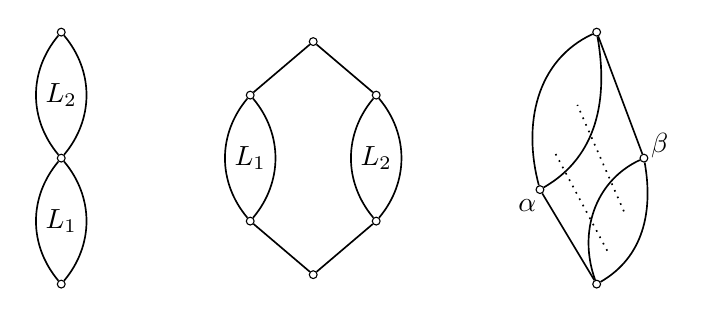
\begin{tikzpicture}[scale=0.4]

      %%% first (unlabelled) parachute %%%
      \node (botL1) at (-8,-4) [draw, circle,inner sep=1pt] {};
      \node (m80) at (-8,0) [draw, circle,inner sep=1pt] {};
      \node (topL2) at (-8,4) [draw,circle,inner sep=1pt] {};
      \node (bot) at (0,-3.7) [draw, circle,inner sep=1pt] {};
      \node (top) at (0,3.7) [draw,circle,inner sep=1pt] {};
      \node (botL) at (-2,-2) [draw,circle,inner sep=1pt] {};
      \node (topL) at (-2,2) [draw,circle,inner sep=1pt] {};
      \node (botN) at (2,-2) [draw,circle,inner sep=1pt] {};
      \node (topN) at (2,2) [draw,circle,inner sep=1pt] {};

      \draw (-8,-2) node {$L_1$};
      \draw (-8,2) node {$L_2$};
      \draw (-2,0) node {$L_1$};
      \draw (2,0) node {$L_2$};

      \draw[semithick] 
      (bot) to (botL)
      (bot) to (botN)
      (top) to (topL)
      (top) to (topN);

      \draw [semithick]  
      (botL) to [out=50,in=-50] (topL)
      (botL) to [out=130,in=-130] (topL)
      (botN) to [out=50,in=-50] (topN)
      (botN) to [out=130,in=-130] (topN);

      \draw [semithick]  
      (botL1) to [out=50,in=-50] (m80)
      (botL1) to [out=130,in=-130] (m80)
      (m80) to [out=50,in=-50] (topL2)
      (m80) to [out=130,in=-130] (topL2);

      % lat5
      \node (c) at (9.5,-3.25)   {};
      \node (d) at (7.5,0.5)   {};
      \node (e) at (10,-2)   {};
      \node (f) at (8.25,2)   {};
      \node (bottom) at (9,-4)  [draw, circle, inner sep=1pt] {};
      \node (topfi) at (9,4)  [draw, circle, inner sep=1pt] {};
      \node (alpha) at (7.2,-1)  [draw, circle, inner sep=1pt] {};
      \node (beta) at (10.5,0)  [draw, circle, inner sep=1pt] {};
      \draw[semithick, dotted] (c) to (d) (e) to (f);
      \draw[semithick] (bottom) to (alpha)  (beta) to (topfi);
      \draw[semithick] 
      (alpha) to [out=30, in=-80] (topfi)
      (topfi) to [out=205, in=105] (alpha)
      (bottom) to [out=30, in=-80] (beta)
      (beta) to [out=205, in=110] (bottom);
      \draw (6.8,-1.5) node {$\alpha$};
      \draw (11,0.4) node {$\beta$};

    \end{tikzpicture}
    \caption{The ordinal (left) and parallel (middle) sum of the lattices
      $L_1$ and $L_2$; a sublattice obtained as a union of a filter $\alpha^\uparrow $ and an ideal
      $\beta^\downarrow$ (right).}
  \end{figure}
\end{center}

\begin{remarks}
  %%   ~
  %% \begin{enumerate} %[label=$\circ$]
  %% \item  The first result says that if $L$ is representable then so is the
  The first item in the list above says that if $L$ is representable then so is the dual of $L$. 
  It follows from this that any interval sublattice of a representable lattice is
  representable.  For, let $[\alpha, \beta] := \{\theta \in L \mid \alpha \leq
  \theta \leq \beta\}$ be an interval in the representable lattice $L= \Con\bA$.
  Then $[\alpha, 1_A] \cong \Con \bA/\alpha$. By 1, the dual of $\ell := [\alpha, 1_A]$ is
  representable. %say, $\ell' = \Con \bB$. 
  Now take the filter above $\beta'$ in $\ell'$ (where $\beta'$ is the
  image of $\beta$ under dualization) and we obtain a representation of a
  lattice isomorphic to the dual of $[\alpha, \beta]$.  Apply 1
  again and we have the desired representation of $[\alpha, \beta]$.  Thus
  2 follows from 1.
  By the ordinal sum of two lattices $L_1, L_2$, we mean the lattice
  on the left of Figure~\ref{fig:ordinal-and-parallel}.
  By the parallel sum of two lattices $L_1, L_2$, we mean the lattice
  in the middle of Figure~\ref{fig:ordinal-and-parallel}.
  %% \item[4.-5.] By the
  %%   ordinal (parallel) sum of two lattices $L_1, L_2$, we mean the lattice
  %%   on the left (middle) of Figure~\ref{fig:ordinal-and-parallel}.
  Item 6 above is a very useful result which we will discuss it further in
  Section~\ref{sec:union-filter-ideal} below, where we present a short proof of
  this result. 
  Whether the class $\sL$ is closed under homomorphic images
  seems to be an open question. 
\end{remarks}

%%%%%%%%%%%%%%%%%%  METHODSINDETAIL  %%%%%%%%%%%%%%%%%%%%%%%
\subsection{Lattice duals: the theorem of Kurzweil and Netter}
\label{sec:duals-interv-subl-detail}
As mentioned above, 
the class $\sL$ -- the lattices isomorphic to congruence lattices of finite
algebras -- is closed under
dualization.
That is, if $L$ is representable, then so is the dual of $L$. This was proved in
1986 by Raimund Netter~\cite{Netter:1986}, generalizing the idea of his advisor,
Hans Kurzweil~\cite{Kurzweil:1985}. 
Though Kurzweil's article did appear (in German), it is unclear whether Netter's
article was ever published.
In this section we present a proof of their result.
The argument requires a fair bit of machinery, but it is a nice idea and
well worth the effort.\footnote{We learned 
  of the main argument used in the proof from slides of a series of three
  lectures given by P{\'e}ter \Palfy in 2009~\cite{Palfy:2009}.
  \Palfy gives credit for the argument to Kurzweil and Netter.} 

If $G$ is a group and $X$ a set, then the set $\{f \mid X\rightarrow G\}$ of 
functions from $X$ into $G$ is denoted by $G^X$.  This is a group with binary
operation $(f,g) \mapsto f\cdot g$, where,  
for each $x\in X$, $(f\cdot g)(x)= f(x)g(x)$ is simply multiplication
in the group $G$.  The identity of the group $G^X$ is of course the constant map $f(x) =
1_G$ for all $x\in X$.

Let $X$ be a finite totally ordered set, with order relation $\leq$,
and consider the set $X^X$ of functions mapping $X$ into itself.  
The subset of $X^X$ consisting of functions that are both idempotent and
decreasing\footnote{When we say that the map $f$ is ``decreasing'' we mean
  $f(x)\leq x$ for all $x$. (We do not mean $x\leq y$ implies $f(y) \leq f(x)$.)}
will be denoted by $\ID{X}$.  That is,
\[
\ID{X} = \{f\in X^X \mid f^2 = f \text{ and }\; \forall x\; f(x) \leq x\}.
\]
Define a partial order $\sqsubseteq$ on the set $\ID{X}$ by
\begin{equation}
  \label{eq:MID111}
  f\sqsubseteq g \quad \Leftrightarrow \quad \ker f \leq \ker g,
\end{equation}
where $\ker f = \{(x,y) \mid f(x) = f(y)\}$.
It is easy to see that $f\sqsubseteq g$ holds if and only if $gf = g$.  
Moreover, under this partial ordering $\ID{X}$ is a lattice which is 
isomorphic to $\bEqX$ (viz.~the map $\Theta : \EqX \rightarrow
\ID{X}$ given by $\Theta(\alpha) = f_\alpha$, where
$f_\alpha(x) = \min\{y\in X \mid (x,y)\in \alpha\}$.) % = \min x/\alpha.


Suppose $S$ is a finite nonabelian simple
group, and consider $S^n$, the direct power of $n$ copies of $S$.
An element of $S^n$ may be viewed as a map from the set 
$n = \{0, 1, \dots, n-1\}$ into $S$.  Thus, if 
$x = (x_0, x_1, \dots, x_{n-1})\in S^n$, then by 
$\ker x$ we mean the relation $(i,j) \in \ker x$ if and only if $x_i = x_j$.
The set of constant maps is a subgroup $D < S^n$, sometimes called the
\defn{diagonal subgroup}; that is,
$D = \{(s, s, \dots, s) \mid s\in S\} \leq S^n$.

For each $f \in \ID{n}$, define
\[
K_f = \{(x_{f(0)}, x_{f(1)}, \dots, x_{f(n-1)}) \mid x_{f(i)}\in S, \; i = 0, 1,
\dots, n-1\}.
\]
Then $D \leq K_f\leq S^n$, and $K_f$ is the set of maps
$K_f = \{x f \in S^n \mid x \in S^n \}$; i.e., compositions of the given
map $f\in n^n$, followed by  any $x\in S^n$.  Thus, 
$K_f = \{ y\in S^n \mid \ker f \leq \ker y \}$.
For example, 
if $f = (0, 0, 2, 3, 2)\in \ID{5}$, then 
$\ker f = |0,1|2,4|3|$ and 
$K_f$ is the subgroup %$\Delta \leq K_f \leq S^5$ 
of all $(y_0, y_1, \dots, y_4)\in S^5$ having $y_0 = y_1$ and $y_2 = y_4$. That is,
$K_f = \{(x_{0}, x_{0}, x_2, x_3, x_2) \mid x\in S^5\}$.

\begin{lemma}
  \label{lem:latt-duals}
  The map $f \mapsto K_f$ is a dual lattice isomorphism from $\bEq(n)$ onto the
  interval sublattice $[D, S^n] \leq \Sub(S^n)$.
\end{lemma}
\begin{proof}
  This is clear since $\ID{n}$ is ordered by (\ref{eq:MID111}), and 
  we have 
  $f\sqsubseteq h$ if and only if
  $K_h = \{y \in S^n \mid \ker h \leq \ker y \}
  \leq \{y \in S^n \mid \ker f \leq \ker y \} =  K_f$.
\end{proof}

\begin{theorem}[Kurzweil~\cite{Kurzweil:1985}, Netter~\cite{Netter:1986}]
  \label{thm:duals-interv-subl}
  If the finite lattice $L$ is representable (as the congruence lattice of a
  finite algebra), then so is the dual lattice $L'$.
\end{theorem}
\begin{proof}
  Without loss of generality, we assume that $L$ is represented
  as $L = \Con \<n, F\>$.
  Also, by \cite[Theorem~4.18]{alvi:1987}, we can assume
  that $F$ consists of unary operations: $F \subseteq n^n$.  
  As above, let $S$ be a nonabelian simple group
  and let $D$ be the diagonal subgroup of $S^n$.
  Then the unary algebra $\<S^n/D, S^n\>$  is a transitive $S^n$-set which (by
  Theorem~\ref{thm:g-set-isomorphism2} below) has congruence lattice isomorphic
  to the interval $[D, S^n]$.  By Lemma~\ref{lem:latt-duals}, this is the dual
  of the lattice $\bEq(n)$.  That is, 
  $\Con \<S^n/D, S^n\> \cong (\bEq(n))'$.

  \todo{Replace the reference to Theorem~\ref{thm:g-set-isomorphism2} with a
    reference to the appropriate theorem in ALVIN, since the section containing
    Theorem~\ref{thm:g-set-isomorphism2} below will be deleted.}

  
  Now, each operation $\phi \in F$ gives rise to an operation on $S^n$
  by composition:
  \[
  \hat{\phi}(\bs) = \hat{\phi}(s_{0}, s_1  \dots, s_{n-1}) = (s_{\phi(0)},
  s_{\phi(1)}\dots, s_{\phi(n-1)}). 
  \]
  Thus, $\phi$ induces  an operation on $S^n/D$ since, for 
  $\bd = (d, d, \dots, d) \in D$ and $\bs \in S^n$ we have 
  $\bs \bd = (s_{0}d, s_{1}d, \dots , s_{n-1}d)$ and 
  $\hat{\phi}(\bs \bd) = (s_{\phi(0)}d, s_{\phi(1)}d, \dots , s_{\phi(n-1)}d) = \hat{\phi}(\bs) \bd$,
  so $\hat{\phi}(\bs D)  = \hat{\phi}(\bs) D$.  Finally, add the set of operations 
  $\hat{F} = \{\hat{\phi} \mid \phi \in F\}$ to $\<S^n/D, S^n\>$, yielding the
  new algebra  $\<S^n/D, S^n \cup \hat{F}\>$, and observe
  that a congruence $\theta \in \Con\<S^n/D, S^n\>$ remains a congruence of
  $\<S^n/D, S^n \cup \hat{F}\>$ if and only if it correponds to a partition on
  $n$ that is invariant under $F$.
\end{proof}

\todo{Perhaps we should give more details in the last sentence of the proof.}
%   Some notes are below, but they need to be cleaned up.}

%% {\it Notes on the last sentence of the proof:}
%% Fix 
%% $\theta \in \Con \< S^{n}/D, S^{n}\> \cong [D, S^n]$.  Then\footnote{This,
%%   and more generally the isomorphism $\Con \< S^{n}/D, S^{n}\> \cong [D, S^n]$
%%   follows from Theorem~\ref{thm:g-set-isomorphism2} below.} there corresponds a
%% subgroup $D \leq K_f \leq S^n$ such that 
%% $(x,y)\in \theta$ iff $x^{-1}y = z\in K_f$.  Now if $\hat{\phi}\in \hat{F}$, then
%% $(\hat{\phi}x, \hat{\phi}y) \in \theta$ iff 
%% \[
%% (x_{\phi(0)}^{-1}y_{\phi(0)}, \dots,  x_{\phi(n-1)}^{-1} y_{\phi(n-1)}) =
%% (z_{\phi(0)},z_{\phi(1)},\dots, z_{\phi(n-1)})\in K_f.
%% \]
%% Better: Take $z\in K_f$ with $\ker z = \ker f$, so $f(i)=f(j)$ iff $z_i = z_j$.
%% Now suppose $\phi\in F$ does not respect $\ker f$, so there exists $(i,j) \in
%% \ker f$ such that $(\phi(i), \phi(j)) \notin \ker f$.  Then $\phi z \notin K_f$,
%% since $z_{\phi(i)} \neq z_{\phi(j)}$.

\subsection{Union of a filter and ideal}
\label{sec:union-filter-ideal}
The lemma in this section was originally proved by John Snow using primitive positive
formulas.  Since it provides such a useful tool for proving that certain finite lattices 
are representable as congruence lattices, we give our own direct
proof of the result below. 

Before stating the lemma, we need a couple of definitions.  (These will be
discussed in greater detail in Section~\ref{sec:closure-method}.)
Given a relation $\theta \subseteq X\times X$, we say that the map 
$f: X^n\rightarrow X$ \emph{respects} $\theta$ and we write 
$f(\theta) \subseteq \theta$ provided $(x_i, y_i)\in \theta$ implies
$(f(x_1, \dots, x_n), f(y_1, \dots, y_n))\in \theta$.
For a set $L\subseteq \Eq X$ of equivalence relations we define
\[
\lambda(L) = \{f\in X^X: (\forall \theta \in L) \; f(\theta) \subseteq \theta \},
\]
which is the set of all unary maps on $X$ which respect all relations in $L$.
\begin{lemma} 
  \label{lemma:union-filter-ideal}
  Let $X$ be a finite set.
  If $\bL \leq \bEqX$ is representable and $\bL_0\leq \bL$ is a sublattice with universe
  $\upalpha\cup \downbeta$ where $\upalpha=\{x\in L \mid \alpha \leq x\}$ and 
  $\downbeta=\{x\in L \mid x\leq \beta\}$ for some $\alpha, \beta \in L$, then $\bL_0$ is representable.
\end{lemma}

\vskip3mm

\begin{center}
  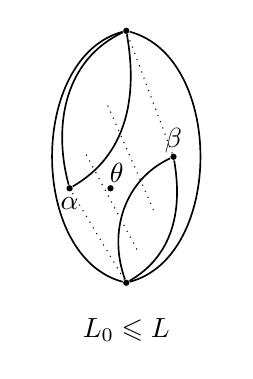
\begin{tikzpicture}[scale=.4]
    % lat5
    \node (c) at (.5,.75)   {};
    \node (d) at (-1.5,4.5)   {};
    \node (e) at (1,2)   {};
    \node (f) at (-.75,6)   {};
    \node (bottom) at (0,0)  [fill, circle, inner sep=.8pt] {};
    \node (top) at (0,8)  [fill, circle, inner sep=.8pt] {};
    \node (alpha) at (-1.8,3)  [fill, circle, inner sep=.8pt] {};
    \node (beta) at (1.5,4)  [fill, circle, inner sep=.8pt] {};
    \node (theta) at (-.5,3)  [fill, circle, inner sep=.8pt] {};
    \draw (-.3,3.5) node {$\theta$};
    \draw[semithick] 
    (bottom) to [out=15, in=-15] (top) 
    (top) to [out=195, in=165] (bottom);
    \draw[dotted] (c) to (d) (e) to (f);
    \draw[dotted] (bottom) to (alpha)  (beta) to (top);
    \draw[semithick] 
    (alpha) to [out=30, in=-80] (top)
    (top) to [out=205, in=105] (alpha)
    (bottom) to [out=30, in=-80] (beta)
    (beta) to [out=205, in=110] (bottom);
    \draw (0,-1.5) node {$L_0 \leq  L$};
    \draw (-1.8,2.5) node {$\alpha$};
    \draw (1.5,4.5) node {$\beta$};
  \end{tikzpicture}
\end{center}

\vskip3mm

\begin{proof}
  Assume $\bL_0 \ncong \two$, otherwise the result holds trivially. 
  Since $\bL\leq \bEqX$ is representable, we have $\bL = \bCon
  \<X, \lambda(L)\>$ (cf.~Section~\ref{sec:closure-method}).  Take an arbitrary
  $\theta \in L \setminus L_0$. Since $\theta \notin \upalpha$, 
  % -- that is, $\alpha$ is not below $\theta$ --  
  there is a pair 
  $(a,b) \in \alpha \setminus \theta$.  Since $\theta \notin \downbeta$, there is
  a pair $(u,v)\in \theta\setminus \beta$. Define $h\in X^X$ as follows:
  \begin{equation*}
    h(x) = \begin{cases}
      a,& \quad x\in u/\beta,\\
      b,& \quad \text{ otherwise.}
    \end{cases}
  \end{equation*}
  Then, $\beta \leq \ker h = (u/\beta)^2 \cup ((u/\beta)^c)^2$, where $(u/\beta)^c$ denotes the
  complement of the $\beta$ class containing $u$.  Therefore, $h$ respects every
  $\gamma \leq \beta$.  Furthermore, $(a, b) \in \gamma$ for all $\gamma \geq \alpha$,
  so $h$ respects every $\gamma$ above $\alpha$.  This proves that $h\in \lambda(L_0)$.
  Now, $\theta$ was arbitrary, so we have proved that for every $\theta \in L
  \setminus L_0$ there exists a function in $\lambda(L_0)$ which respects every
  $\gamma \in \upalpha\cup \downbeta = L_0$, but violates $\theta$.  Finally,
  since 
  $\bL_0 \leq \bL$, we have $\lambda(L)\subseteq \lambda(L_0)$.  Combining these
  observations, we see that every $\theta \in \Eq X \setminus L_0$ is
  violated by some function in $\lambda(L_0)$. Therefore, $\bL_0 = \bCon \< X, \lambda(L_0)\>$.
\end{proof}

\subsection{Ordinal Sums I}
\label{sec:ordinal-sums}
\todo{Revise this section.  Peter has written up some nice lemmas and
  theorems on this topic which now appear below in a subsection called
  ``Ordinal Sums II,'' but that material should be integrated with and/or
  replace the material in this subsection.} 

The following theorem is a consequence of 
McKenzie's shift product construction~\cite{McKenzie:1984}. %, which we describebriefly below.
% \todo{Possibly add a short description of the shift product.}
\begin{theorem}
  \label{thm:ordinal-sums}
  If $L_1, \dots, L_n \in \sL$ is a collection of representable lattices, then
  the ordinal sum and the adjoined ordinal sum, shown in
  Figure~\ref{fig:adjordinal}, are representable.
\end{theorem}
A more direct proof of Theorem~\ref{thm:ordinal-sums} follows the argument given
by John Snow in~\cite{Snow:2000}.  As noted above, 
\Jiri \Tuma proved that
the class of finite representable lattices is closed under direct products.
Thus, if $L_1$ and 
$L_2$ are representable, then so is $L_1 \times L_2$.  Now note that the
adjoined ordinal sum of $L_1$ and $L_2$ is the union, $\alpha^\uparrow \cup
\beta^\downarrow$,  of a filter and ideal  
in the lattice $L_1 \times L_2$, where
$\alpha = \beta = 1_{L_1} \times 0_{L_2}$.  
Therefore, by Lemma~\ref{lemma:union-filter-ideal},
the adjoined ordinal sum is representable.  A trivial induction argument proves the
result for adjoined ordinal sums of $n$ lattices.  The same result for ordinal
sums (Figure~\ref{fig:adjordinal} left) follows since the two element lattice is
obviously representable. 

\begin{center}
  \begin{figure}[h!]
    \label{fig:adjordinal}
    \centering
        {\scalefont{.8}
          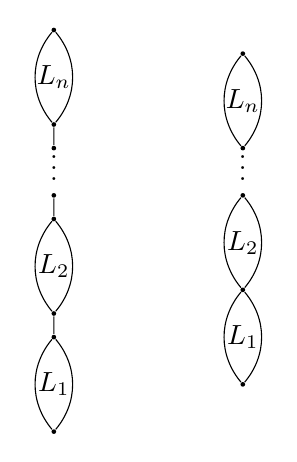
\begin{tikzpicture}[scale=0.3]
            \node (botL1) at (8,-4) [fill, circle,inner sep=.6pt] {};
            \node (00) at (8,0) [fill, circle,inner sep=.6pt] {};
            \node (topL2) at (8,4) [fill,circle,inner sep=.6pt] {};
            \node (topLn) at (8,10) [fill, circle,inner sep=.6pt] {};
            \node (botLn) at (8,6) [fill, circle,inner sep=.6pt] {};

            \draw (8,-2) node {$L_1$};
            \draw (8,8) node {$L_n$};
            \draw (8,2) node {$L_2$};
            \draw (8,5.5) node {$\vdots$};

            \draw 
            (botL1) to [out=50,in=-50] (00)
            (botL1) to [out=130,in=-130] (00)
            (00) to [out=50,in=-50] (topL2)
            (00) to [out=130,in=-130] (topL2)
            (botLn) to [out=50,in=-50] (topLn)
            (botLn) to [out=130,in=-130] (topLn);

            \node (botL1) at (0,-6) [fill, circle,inner sep=.6pt] {};
            \node (topL1) at (0,-2) [fill, circle,inner sep=.6pt] {};
            \node (botL2) at (0,-1) [fill, circle,inner sep=.6pt] {};
            \node (topL2) at (0,3) [fill,circle,inner sep=.6pt] {};
            \node (04) at (0,4) [fill, circle,inner sep=.6pt] {};
            \node (06) at (0,6) [fill, circle,inner sep=.6pt] {};
            \node (botLn) at (0,7) [fill, circle,inner sep=.6pt] {};
            \node (topLn) at (0,11) [fill, circle,inner sep=.6pt] {};

            \draw (0,-4) node {$L_1$};
            \draw (0,9) node {$L_n$};
            \draw (0,1) node {$L_2$};
            \draw (0,5.5) node {$\vdots$};

            \draw 
            (botL1) to [out=50,in=-50] (topL1)
            (botL1) to [out=130,in=-130] (topL1) 
            to (botL2) to [out=50,in=-50] (topL2)
            (botL2) to [out=130,in=-130] (topL2)
            (topL2) to (04)
            (06) to (botLn) to [out=50,in=-50] (topLn)
            (botLn) to [out=130,in=-130] (topLn);
          \end{tikzpicture}
        }
        \caption{The ordinal sum (left) and the adjoined ordinal sum (right) of the lattices
          $L_1, \dots, L_n$.}
  \end{figure}
\end{center}

\subsection{Ordinal Sums II}
\todo{Merge this subsection with the subsection ``Ordinal Sums I.''}
\newcommand{\m}{\mathbf}

The lattice of equivalence relations on an $n$-element set is denoted by
Equ$(n)$. For two lattices $\m L,\m M$ the \emph{adjoined ordinal sum}  
is denoted by $\m L\oplus_a \m M$ and is defined on $L\uplus (M\setminus\{0\})$
by $x\le y$ iff $x\in L,y\in M$ or ($x,y\in L$ and $x\le^\m L y$) or ($x,y\in M$
and $x\le^\m M y$). 

Let $\m A,\m B$ be two finite algebras of cardinality $m$ and $n$ respectively,
and let $\m L=\text{Con}(\m A)$ and $\m M=\text{Con}(\m B)$. 
In \cite{Snow:2000} it is proved that $\m L\oplus_a\m M$ is isomorphic to the
congruence lattice of some finite algebra $\m C$. Although the algebra $\m C$ is
not explicitly constructed, it is based on the direct product of $\m A$ and $\m
B$, hence the ordinal sum is a sublattice of Equ$(mn)$. Here we give a different
construction of $\m C$ that leads to a tighter representation of Con$(\m C)$ as
a sublattice of Equ$(m+n-1)$.  
%If $\m A$ and $\m B$ are minimal-size algebras that have congruence lattices
%isomorphic to $\m L$ and $\m M$ respectively, then $\m C$ will also be a
%minimal-size algebra with congruence lattice isomorphic to $\m L\oplus_a\m M$. 

Define a unary algebra $\m A_{m,n}$ with $m+n-1$ elements as follows: 
the base set is $A\uplus B_1$ where $A=\{a_0,\dots,a_{m-1}\}$,
$B_1=\{b_1,\dots,b_{n-1}\}$ and for each function $h:B_1\to A$ define a unary
operation 
$$\hat h(x)=\begin{cases}h(x)&\text{if $x\in B_1$}\\ 
x&\text{otherwise.}\end{cases}$$

\begin{lemma}
  For $m,n\ge 1$ the lattice $\mathrm{Con}(\m A_{m,n})$ is isomorphic to
  $\mathrm{Equ}(m)\oplus_a \mathrm{Equ}(n)$. 
\end{lemma}
\begin{proof}
  Let $\alpha$ be the equivalence relation
  $A^2\cup\{(b_1,b_1),\dots,(b_{n-1},b_{n-1})\}$, so as a partition it is  
  $a_0,\dots,a_{m-1}|b_1|b_2|\dots|b_{n-1}$. 
  Note that Equ$(m)\oplus_a \text{Equ}(n)$ is isomorphic to the sublattice
  of Equ$(A\uplus B_1)$ of all equivalence relations comparable to $\alpha$, since
  $\alpha$ has a unique non-singleton block of size $m$, and $n$ blocks
  altogether. We claim that this sublattice is the congruence lattice of $\m
  A_{m,n}$.  

  Suppose $\theta\le\alpha$, and let $(x,y)\in\theta$. Then $x,y\in A$ or $x=y$,
  hence for any operation $\hat h$ we  have $\hat h(x)=x$ and $\hat h(y)=y$ or
  $\hat h(x)=\hat h(y)$, so $(\hat h(x),\hat h(y))\in\theta$. 

  Suppose $\alpha\le\theta$, and let $(x,y)\in\theta$. Since $A^2\subseteq\alpha$
  and since the range of each $\hat h$ is $A$ it follows that 
  $(\hat h(x),\hat h(y))\in\theta$. 

  Now suppose $\theta$ is incomparable with $\alpha$. Then $A^2$ is not a subset
  of $\theta$, hence there exist $(x,y)\in A^2\setminus\theta$ and
  $(u,v)\in\theta\setminus\alpha$. If $u,v\in B_1$ then choose a function $h$ (as
  in the definition of $\m A_{m,n}$) such that $h(u)=x$ and $h(v)=y$, in which
  case $\hat h$ is an operation that shows $\theta$ is not a congruence. 
  If $u\in B_1$, but $v\in A$, note that we cannot have both $(x,v)$ and $(y,v)$
  in $\theta$ (else $(x,y)\in\theta$). Assume without loss of generality 
  that $(x,v)\notin\theta$ and choose $h$ such that $h(u)=x$, then again $\hat h$
  shows that $\theta$ is not a congruence. 
  The case $u\in A$, $v\in B_1$ is similar, and $u,v\in A$ is excluded since
  $(u,v)\notin\alpha$. 
\end{proof}

%\newpage

\begin{theorem}
  Suppose $\m A=(A,F)$ and $\m B=(B,G)$ are unary algebras with
  $A=\{a_0,\dots,a_{m-1}\}$, $B=\{b_0,\dots,b_{n-1}\}$ and 
  $A\cap B=\{a_0\}=\{b_0\}$ $($so $a_0,b_0$ are identified$)$. Let $\m C$ be the
  algebra $\m A_{m,n}$ expanded with the operations 
  $$
  \hat f(x)=\begin{cases}f(x)&\text{if $x\in A$}\\
  f(a_0)&\text{otherwise}\end{cases}\qquad\qquad
  \hat g(x)=\begin{cases}g(x)&\text{if $x\in B$}\\
  g(b_0)&\text{otherwise}\end{cases}
  $$
  for $f\in F$ and $g\in G$. Then $\mathrm{Con}(\m C)$ is isomorphic to
  $\mathrm{Con}(\m A)\oplus_a\mathrm{Con}(\m B)$. 
\end{theorem}

\begin{proof}
  Since $\m C$ is an expansion of $\m A_{m,n}$ it follows from the preceding lemma
  that Con$(\m C)$ is a sublattice of 
  $\{\theta\in \text{Equ}(A\cup B):\theta\le\alpha$ or $\alpha\le\theta\}$ where,
  as before, $\alpha=A^2\cup\text{id}_B$. Note that $\alpha\in\text{Con}(\m C)$,
  so it suffices to show that $\{\theta\in\text{Con}(\m C):\theta\le\alpha\}$ is
  isomorphic to Con$(\m A)$ and $\{\theta\in\text{Con}(\m C):\theta\le\alpha\}$ 
  is isomorphic to Con$(\m B)$. The second isomorphism follows from the
  observation that $\m C/\alpha$ is isomorphic to $\m B$ via the map 
  $A\mapsto b_0$ and $\{b_i\}\mapsto b_i$ for $i\ge 1$. For the first isomorphism,
  note that the operations $\hat g$, $\hat h$ preserve all equivalence relations
  below $\alpha$. Similarly it is straight forward to check that $\hat f$
  preserves $\theta\le\alpha$ iff $f$ preserves $\theta\cap A^2$. 
  Hence the map $\theta\mapsto\theta\cap A^2$ is the required isomorphism.
\end{proof}

Now assume $\m A$ and $\m B$ are minimal-size algebras with congruence lattices
isomorphic to $\m L$ and $\m M$ respectively. Then it seems likely that the
algebra $\m C$ above is minimal in size with respect to having a congruence
lattice isomorphic to $\m L\oplus_a\m M$. Suppose $\m C'$ is a smaller algebra
with the same congruence lattice, and let $\alpha$ be the congruence in the
``middle'' of the ordinal sum. Then $\m C'/\alpha$ has a congruence lattice
isomorphic to $\m M$, hence $|\m C'/\alpha|=|\m B|=$ number of blocks in
$\alpha$. However, $\alpha$ does not need to have a unique nontrivial block, so
it is not clear at the moment how to obtain a smaller algebra $\m A'$ such that
Con$(\m A')$ is isomorphic to $\m L$. 


  (include all major inputs in one file)
%% -- Begin intro.tex file insertion -------------------------------


%%%%%%%%%%%%%%%%%  NOTATION %%%%%%%%%%%%%%%%%%%%%%%%%%%%%%%%

\subsection{Notation}

Throughout this paper, we use $\sL$ to denote the class of finite lattices that
are isomorphic to congruence lattices of finite algebras. 
We call the lattices that belong to $\sL$ \emph{representable} lattices. 

Let $L$ be a lattice and suppose $\alpha$ and $\beta$ belong to $L$.  
We denote by $\lb \alpha, \beta \rb$ the sublattice of $L$ consisting of all elements in $L$
that lie above $\alpha$ and below $\beta$.  
That is, 
$\lb \alpha, \beta \rb = 
\{\theta \in L \mid \alpha \leq \theta \text{ and } \theta \leq \beta\}$.
(If $\alpha \nleq \beta$, then $\lb \alpha, \beta \rb = \emptyset$.)

For a lattice (or, more generally, a partially ordered set) 
$L$, the \emph{dual} of $L$, denoted
$L'$, is the lattice (poset) with the inverse order. That is, 
$x \leq y$ holds in $L$ if and only if $y \leq x$ holds in $L'$. 
The dual of $L$ can be depicted by flipping the Hasse diagram
for $L$ upside down. 
In a broader sense, two lattices (posets) are also said to be duals if they are
dually isomorphic.
Although we often denote the dual of $L$ by $L'$, on some occasions it is more
convenient to use an operator notation, such as $\partial L$, to denote the dual of
$L$. 

%%%%%%%%%%%%%%%%%  METHODSOVERVIEW %%%%%%%%%%%%%%%%%%%%%%%%%%%%%%%%

\section{Closure properties of the class of representable lattices}
\label{sec:clos-prop-class}
This section describes some
\emph{closure properties}
of the class $\sL$. % of representable lattices. 
By closure properties, we mean the following: if $\sansO$ is an operation that can
be applied to a lattice or collection of lattices, we say that $\sL$ is
\emph{closed under $\sansO$} provided $\sansO(\sK) \subseteq \sL$ for all 
$\sK\subseteq \sL$. For example, if 
$\sansS(\sK)$ is all sublattices of lattices in $\sK$, 
it is unknown whether $\sL$ is closed under $\sansS$.  
If this were known to be true, then the 
\emph{finite lattice representation problem} would be solved.
The congruence lattice of the algebra consisting of a
set $X$ with no operations is the lattice of all equivalence relations on $X$,
which we denote by $\Eq X$.
By a celebrated theorem of \Pudlak and \Tuma~\cite{Pudlak:1980}, for every finite
lattice $L$ there is a finite set $X$ such that $L\leq \Eq X$.  Therefore, $\sL$
would contain all finite lattices if it were closed under $\sansS$.


The following is a list of operations under which $\sL$ is known to be closed,
along with the names of those who first (or independently) proved them.  We
discuss some of these results in greater detail later in this section.
The class $\sL$ of lattices isomorphic to congruence lattices of finite
algebras is closed under the following operations:
\begin{enumerate} %[label=$\circ$]
\item\label{item:1} lattice duals (Hans Kurzweil~\cite{Kurzweil:1985} and Raimund Netter~\cite{Netter:1986}, 1986),
\item interval sublattices (follows from~(\ref{item:1})),
\item  direct products (\Jiri \Tuma~\cite{Tuma:1986}, 1986), 
\item  ordinal sums 
  (Ralph McKenzie~\cite{McKenzie:1984}, 1984; John Snow~\cite{Snow:2000}, 2000),
\item  parallel sums (John Snow~\cite{Snow:2000}, 2000), 
\item certain sublattices of lattices in $\sL$ -- namely, those which
  are obtained as a union of a filter and an ideal of a lattice in
  $\sL$ (John Snow~\cite{Snow:2000}, 2000). 
\end{enumerate}
\begin{center}
  \begin{figure}[h!]
    \centering
    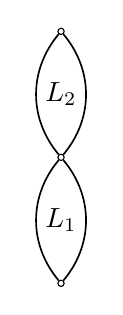
\begin{tikzpicture}[scale=0.4]
      %% file: ordinal-sum.tex
%% author: williamdemeo@gmail.com
%% To insert this in a document, put it inside a tikzpicture block. 
%% 
%% notes: two potatoes, one atop the other

\node (botL1) at (0,-4) [draw, circle,inner sep=\dotsize] {};
\node (m80) at (0,0) [draw, circle,inner sep=\dotsize] {};
\node (topL2) at (0,4) [draw,circle,inner sep=\dotsize] {};

\draw [semithick]  
(botL1) to [out=50,in=-50] (m80)
(botL1) to [out=130,in=-130] (m80)
(m80) to [out=50,in=-50] (topL2)
(m80) to [out=130,in=-130] (topL2);

%% If you get undefined control sequence \dotsize when you compile, put
%% the following command in the preamble of your document:
%% \newcommand{\dotsize}{1pt}


      \draw (0,-2) node {$L_1$};
      \draw (0,2) node {$L_2$};
    \end{tikzpicture}
    \hskip5mm
    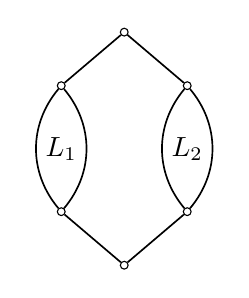
\begin{tikzpicture}[scale=0.4]
      %% file: parallel-sum.tex
%% author: williamdemeo@gmail.com
%% To insert this in a document, put it inside a tikzpicture block. 

%% notes: Two potatoes side-by-side with new common top and bottom
\node (bot) at (0,-3.7) [draw, circle,inner sep=1pt] {};
\node (top) at (0,3.7) [draw,circle,inner sep=1pt] {};
\node (botL1) at (-2,-2) [draw,circle,inner sep=1pt] {};
\node (topL1) at (-2,2) [draw,circle,inner sep=1pt] {};
\node (botL2) at (2,-2) [draw,circle,inner sep=1pt] {};
\node (topL2) at (2,2) [draw,circle,inner sep=1pt] {};

\draw[semithick] 
(bot) to (botL1) (topL1) to (top)
(bot) to (botL2) (topL2) to (top);

\draw [semithick]  
(botL1) to [out=50,in=-50] (topL1)
(botL1) to [out=130,in=-130] (topL1)
(botL2) to [out=50,in=-50] (topL2)
(botL2) to [out=130,in=-130] (topL2);


      \draw (-2,0) node {$L_1$};
      \draw (2,0) node {$L_2$};
    \end{tikzpicture}
    \hskip5mm
    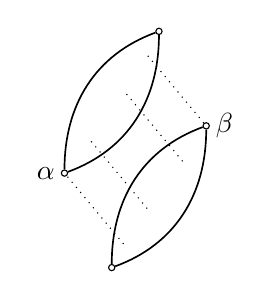
\begin{tikzpicture}[scale=0.3]
      %% file: filter-ideal.tex
%% author: williamdemeo@gmail.com
%% To insert this in a document, put it inside a tikzpicture block. 

%% Disjoint union of a principal filter and a principle ideal.
\node[lat] (bot) at (0,0) {};
\node[lat] (top) at (2,10) {};
\node[lat] (alpha) at (-2,4) {};
\node[lat] (beta) at (4,6) {};
\draw[semithick] 
% filter:
(alpha) to [out=20, in=-90] (top)
(alpha) to [out=90, in=200] (top)
% ideal: 
(bot) to [out=20, in=-90] (beta)
(bot) to [out=90, in=200] (beta);


%% dotted lines suggest ordering of elements in distinct potatoes
%% To remove the dotted lines, comment the next two lines:
\draw[dotted] 
(0.5,1) to (alpha)
(1.5,2.5) to (-1,5.5)
(3,4.5) to (0.5,7.5)
(beta) to (1.5,9);



      \draw (alpha) node [left] {$\alpha$};
      \draw (beta) node [right] {$\beta$};
    \end{tikzpicture}
    \caption{The adjoined ordinal sum (left) and parallel sum (middle) 
      of the lattices $L_1$ and $L_2$; a union of an order filter
      $\alpha^\uparrow$ and order ideal $\beta^\downarrow$ (right).}
    \label{fig:ord_par_fil-uni}
  \end{figure}
\end{center}

\begin{remarks}
  \begin{enumerate}[a.]
  \item 
  The first item in the list above says that if $L$ is representable then so is
  the dual of $L$. It follows from this that every interval sublattice of a
  representable lattice is also representable.  
  Indeed, suppose $L$ is representable, say, $L\cong \bar{L} =\Con\bA$.
  Let $\lb \alpha, \beta \rb$ be an interval sublattice of $L$,
  and $\lb \bar{\alpha}, \bar{\beta} \rb$ the corresponding  
  interval of $\bar{L}$.
  For ease of notation, let's rename $\bar{\alpha}$ and $\bar{\beta}$, dropping
  the bars.  Thus $\lb \alpha, \beta \rb$ is the interval of interest and we
  assume $\lb \alpha, \beta \rb\leq \Con \bA$.
  The filter $\alpha^\uparrow =\lb \alpha, 1_A \rb$ 
  is isomorphic to $\Con (\bA/\alpha)$, hence representable, so
  by~(1) the dual $\partial (\alpha^\uparrow)=\lb 1_A', \alpha'\rb$ is also
  representable. (Here $x'$ denotes the image of $x$ under dualization.)
  Another quotient (this time by $\beta'$) gives a representation of
  the interval $\lb \beta', \alpha'\rb$ above $\beta'$ in 
  $\partial (\alpha^\uparrow)$. 
  Since $\lb \beta', \alpha' \rb$  is the dual of $\lb \alpha, \beta \rb$, 
  we apply~(1) once more to obtain the desired representation of 
  $\lb \alpha, \beta\rb$.  Thus~(2) follows from~(1).

  \item By the ordinal sum of two lattices $L_1$, $L_2$, we mean the lattice
  on the left of Figure~\ref{fig:ord_par_fil-uni}.
  By the parallel sum of two lattices $L_1$, $L_2$, we mean the lattice
  in the middle of Figure~\ref{fig:ord_par_fil-uni}.

\item Item~(6) above is a very useful result which we will discuss further in
  Section~\ref{sec:union-filter-ideal} below, where we present a short proof of
  this fact.

\item Whether the class $\sL$ is closed under homomorphic images
  seems to be an open question. 
  \end{enumerate}
\end{remarks}

%%%%%%%%%%%%%%%%%%  METHODSINDETAIL  %%%%%%%%%%%%%%%%%%%%%%%
\subsection{Lattice duals: the theorem of Kurzweil and Netter}
\label{sec:duals-interv-subl-detail}
As mentioned above, 
the class $\sL$ -- the lattices isomorphic to congruence lattices of finite
algebras -- is closed under
dualization.
That is, if $L$ is representable, then so is the dual of $L$. This was proved in
1986 by Raimund Netter~\cite{Netter:1986}, generalizing the idea of his advisor,
Hans Kurzweil~\cite{Kurzweil:1985}. 
Though Kurzweil's article did appear,
%(in German), 
it is unclear whether Netter's
article was ever published.
In this section we present a proof of their result.
The argument requires a fair bit of machinery, but it is a nice idea and
well worth the effort.\footnote{We learned 
  of the main argument used in the proof from slides of a series of three
  lectures given by P{\'e}ter \Palfy in 2009~\cite{Palfy:2009}.
  \Palfy gives credit for the argument to Kurzweil and Netter.} 

If $G$ is a group and $X$ a set, then the set $\{f \mid X\rightarrow G\}$ of 
functions from $X$ into $G$ is denoted by $G^X$.  This is a group with binary
operation $(f,g) \mapsto f\cdot g$, where,  
for each $x\in X$, $(f\cdot g)(x)= f(x)g(x)$ is simply multiplication
in the group $G$.  The identity of the group $G^X$ is of course the constant map $f(x) =
1_G$ for all $x\in X$.

Let $X$ be a finite totally ordered set, with order relation $\leq$,
and consider the set $X^X$ of functions mapping $X$ into itself.  
The subset of $X^X$ consisting of functions that are both idempotent and
decreasing in the sense $f(x) \leq x$
%\footnote{When we say that the map $f$ is ``decreasing'' we mean
%  $f(x)\leq x$ for all $x$. (We do not mean $x\leq y$ implies $f(y) \leq f(x)$.)}
will be denoted by $\ID{X}$.  That is,
\[
\ID{X} = \{f\in X^X \mid f^2 = f \text{ and }\; \forall x\; f(x) \leq x\}.
\]
Define a partial order $\sqsubseteq$ on the set $\ID{X}$ by
\begin{equation}
  \label{eq:MID111}
  f\sqsubseteq g \quad \Leftrightarrow \quad \ker f \leq \ker g,
\end{equation}
where of course $\ker f = \{(x,y) \mid f(x) = f(y)\}$.
It is easy to see that $f\sqsubseteq g$ holds if and only if $gf = g$.  
Moreover, under this partial ordering $\ID{X}$ is a lattice which is 
isomorphic to $\bEqX$ (viz.~the map $\Theta : \EqX \rightarrow
\ID{X}$ given by $\Theta(\alpha) = f_\alpha$, where
$f_\alpha(x) = \min\{y\in X \mid (x,y)\in \alpha\}$.) % = \min x/\alpha.


Suppose $S$ is a finite nonabelian simple
group, and consider $S^n$, the direct power of $n$ copies of $S$.
An element of $S^n$ may be viewed as a map from the set 
$n = \{0, 1, \dots, n-1\}$ into $S$.  Thus, if 
$x = (x_0, x_1, \dots, x_{n-1})\in S^n$, then by 
$\ker x$ we mean the relation $(i,j) \in \ker x$ if and only if $x_i = x_j$.
The set of constant maps is a subgroup $D < S^n$, sometimes called the
\defn{diagonal subgroup}; that is,
$D = \{(s, s, \dots, s) \mid s\in S\} \leq S^n$.

For each $f \in \ID{n}$, define
\[
K_f = \{(x_{f(0)}, x_{f(1)}, \dots, x_{f(n-1)}) \mid x_{f(i)}\in S, \; i = 0, 1,
\dots, n-1\}.
\]
Then $D \leq K_f\leq S^n$, and $K_f$ is the set of maps
$K_f = \{x f \in S^n \mid x \in S^n \}$; i.e., compositions of the given
map $f\in n^n$, followed by  any $x\in S^n$.  Thus, 
$K_f = \{ y\in S^n \mid \ker f \leq \ker y \}$.
For example, 
if $f = (0, 0, 2, 3, 2)\in \ID{5}$, then 
$\ker f = |0,1|2,4|3|$ and 
$K_f$ is the subgroup %$\Delta \leq K_f \leq S^5$ 
of all $(y_0, y_1, \dots, y_4)\in S^5$ having $y_0 = y_1$ and $y_2 = y_4$. That is,
$K_f = \{(x_{0}, x_{0}, x_2, x_3, x_2) \mid x\in S^5\}$.

\begin{lemma}
  \label{lem:latt-duals}
  The map $f \mapsto K_f$ is a dual lattice isomorphism from $\bEq(n)$ onto the
  interval sublattice $\lb D, S^n\rb \leq \Sub(S^n)$.
\end{lemma}
\begin{proof}
  This is clear since $\ID{n}$ is ordered by (\ref{eq:MID111}), and 
  we have 
  $f\sqsubseteq h$ if and only if
  $K_h = \{y \in S^n \mid \ker h \leq \ker y \}
  \leq \{y \in S^n \mid \ker f \leq \ker y \} =  K_f$.
\end{proof}

\begin{theorem}[Kurzweil~\cite{Kurzweil:1985}, Netter~\cite{Netter:1986}]
  \label{thm:duals-interv-subl}
  If the finite lattice $L$ is representable (as the congruence lattice of a
  finite algebra), then so is the dual lattice $L'$.
\end{theorem}
\begin{proof}
  Without loss of generality, we assume that $L$ is represented
  as $L = \Con \<n, F\>$.
  Also, by \cite[Theorem~4.18]{alvi:1987}, we can assume
  that $F$ consists of unary operations: $F \subseteq n^n$.  
  As above, let $S$ be a nonabelian simple group
  and let $D$ be the diagonal subgroup of $S^n$.
  Then the unary algebra $\<S^n/D, S^n\>$  is a transitive $S^n$-set which (by
  Theorem~\ref{thm:g-set-isomorphism2} below) has congruence lattice isomorphic
  to the interval $\lb D, S^n\rb$.  By Lemma~\ref{lem:latt-duals}, this is the dual
  of the lattice $\bEq(n)$.  That is, 
  $\Con \<S^n/D, S^n\> \cong (\bEq(n))'$.

  \todo{Replace the reference to Theorem~\ref{thm:g-set-isomorphism2} with a
    reference to the appropriate theorem in ALVIN, since the section containing
    Theorem~\ref{thm:g-set-isomorphism2} below will be deleted.}

  
  Now, each operation $\phi \in F$ gives rise to an operation on $S^n$
  by composition:
  \[
  \hat{\phi}(\bs) = \hat{\phi}(s_{0}, s_1  \dots, s_{n-1}) = (s_{\phi(0)},
  s_{\phi(1)}\dots, s_{\phi(n-1)}). 
  \]
  Thus, $\phi$ induces  an operation on $S^n/D$ since, for 
  $\bd = (d, d, \dots, d) \in D$ and $\bs \in S^n$ we have 
  $\bs \bd = (s_{0}d, s_{1}d, \dots , s_{n-1}d)$ and 
  $\hat{\phi}(\bs \bd) = (s_{\phi(0)}d, s_{\phi(1)}d, \dots , s_{\phi(n-1)}d) = \hat{\phi}(\bs) \bd$,
  so $\hat{\phi}(\bs D)  = \hat{\phi}(\bs) D$.  Finally, add the set of operations 
  $\hat{F} = \{\hat{\phi} \mid \phi \in F\}$ to $\<S^n/D, S^n\>$, yielding the
  new algebra  $\<S^n/D, S^n \cup \hat{F}\>$, and observe
  that a congruence $\theta \in \Con\<S^n/D, S^n\>$ remains a congruence of
  $\<S^n/D, S^n \cup \hat{F}\>$ if and only if it corresponds to a partition on
  $n$ that is invariant under $F$.
\end{proof}

\todo{Perhaps we should give more details in the last sentence of the proof.}
%   Some notes are below, but they need to be cleaned up.}

%% {\it Notes on the last sentence of the proof:}
%% Fix 
%% $\theta \in \Con \< S^{n}/D, S^{n}\> \cong [D, S^n]$.  Then\footnote{This,
%%   and more generally the isomorphism $\Con \< S^{n}/D, S^{n}\> \cong [D, S^n]$
%%   follows from Theorem~\ref{thm:g-set-isomorphism2} below.} there corresponds a
%% subgroup $D \leq K_f \leq S^n$ such that 
%% $(x,y)\in \theta$ iff $x^{-1}y = z\in K_f$.  Now if $\hat{\phi}\in \hat{F}$, then
%% $(\hat{\phi}x, \hat{\phi}y) \in \theta$ iff 
%% \[
%% (x_{\phi(0)}^{-1}y_{\phi(0)}, \dots,  x_{\phi(n-1)}^{-1} y_{\phi(n-1)}) =
%% (z_{\phi(0)},z_{\phi(1)},\dots, z_{\phi(n-1)})\in K_f.
%% \]
%% Better: Take $z\in K_f$ with $\ker z = \ker f$, so $f(i)=f(j)$ iff $z_i = z_j$.
%% Now suppose $\phi\in F$ does not respect $\ker f$, so there exists $(i,j) \in
%% \ker f$ such that $(\phi(i), \phi(j)) \notin \ker f$.  Then $\phi z \notin K_f$,
%% since $z_{\phi(i)} \neq z_{\phi(j)}$.

\subsection{Union of a filter and ideal}
\label{sec:union-filter-ideal}
The lemma in this section was originally proved by John Snow using primitive positive
formulas.  Since it provides such a useful tool for proving that certain finite lattices 
are representable as congruence lattices, we give our own direct
proof of the result below. 

Before stating the lemma, we need a couple of definitions.  (These will be
discussed in greater detail in Section~\ref{sec:closure-method}.)
Given a relation $\theta \subseteq X\times X$, we say that the map 
$f: X^n\rightarrow X$ \emph{respects} $\theta$ and we write 
$f(\theta) \subseteq \theta$ provided $(x_i, y_i)\in \theta$ implies
$(f(x_1, \dots, x_n), f(y_1, \dots, y_n))\in \theta$.
For a set $L\subseteq \Eq X$ of equivalence relations we define
\[
\lambda(L) = \{f\in X^X: (\forall \theta \in L) \; f(\theta) \subseteq \theta \},
\]
which is the set of all unary maps on $X$ which respect all relations in $L$.
\begin{lemma} 
  \label{lemma:union-filter-ideal}
  Let $X$ be a finite set.
  If $\bL \leq \bEqX$ is representable and $\bL_0\leq \bL$ is a sublattice with universe
  $\upalpha\cup \downbeta$ where $\upalpha=\{x\in L \mid \alpha \leq x\}$ and 
  $\downbeta=\{x\in L \mid x\leq \beta\}$ for some $\alpha, \beta \in L$, then $\bL_0$ is representable.
\end{lemma}

\vskip3mm

\begin{center}
  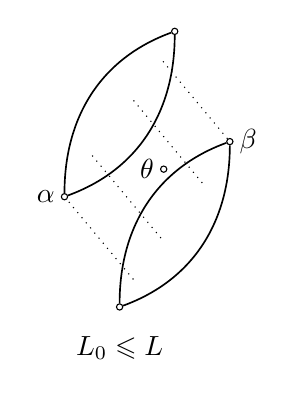
\begin{tikzpicture}[scale=.35]
    %% file: filter-ideal.tex
%% author: williamdemeo@gmail.com
%% To insert this in a document, put it inside a tikzpicture block. 

%% Disjoint union of a principal filter and a principle ideal.
\node[lat] (bot) at (0,0) {};
\node[lat] (top) at (2,10) {};
\node[lat] (alpha) at (-2,4) {};
\node[lat] (beta) at (4,6) {};
\draw[semithick] 
% filter:
(alpha) to [out=20, in=-90] (top)
(alpha) to [out=90, in=200] (top)
% ideal: 
(bot) to [out=20, in=-90] (beta)
(bot) to [out=90, in=200] (beta);


%% dotted lines suggest ordering of elements in distinct potatoes
%% To remove the dotted lines, comment the next two lines:
\draw[dotted] 
(0.5,1) to (alpha)
(1.5,2.5) to (-1,5.5)
(3,4.5) to (0.5,7.5)
(beta) to (1.5,9);



    \draw (0,-1.5) node {$L_0 \leq  L$};
    \draw (alpha) node [left]{$\alpha$};
    \draw (beta) node [right]{$\beta$};
    \node (theta) at (1.6,5)  [draw,circle,inner sep=\dotsize] {};
    %\draw (-.3,3.5) node {$\theta$};
    \draw (theta) node [left]{$\theta$};
  \end{tikzpicture}
\end{center}

\vskip3mm

\begin{proof}
  Assume $\bL_0 \ncong \two$, otherwise the result holds trivially. 
  Since $\bL\leq \bEqX$ is representable, we have $\bL = \bCon
  \<X, \lambda(L)\>$ (cf.~Section~\ref{sec:closure-method}).  Take an arbitrary
  $\theta \in L \setminus L_0$. Since $\theta \notin \upalpha$, 
  % -- that is, $\alpha$ is not below $\theta$ --  
  there is a pair 
  $(a,b) \in \alpha \setminus \theta$.  Since $\theta \notin \downbeta$, there is
  a pair $(u,v)\in \theta\setminus \beta$. Define $h\in X^X$ as follows:
  \begin{equation*}
    h(x) = \begin{cases}
      a,& \quad x\in u/\beta,\\
      b,& \quad \text{ otherwise.}
    \end{cases}
  \end{equation*}
  Then, $\beta \leq \ker h = (u/\beta)^2 \cup ((u/\beta)^c)^2$, where $(u/\beta)^c$ denotes the
  complement of the $\beta$ class containing $u$.  Therefore, $h$ respects every
  $\gamma \leq \beta$.  Furthermore, $(a, b) \in \gamma$ for all $\gamma \geq \alpha$,
  so $h$ respects every $\gamma$ above $\alpha$.  This proves that $h\in \lambda(L_0)$.
  Now, $\theta$ was arbitrary, so we have proved that for every $\theta \in L
  \setminus L_0$ there exists a function in $\lambda(L_0)$ which respects every
  $\gamma \in \upalpha\cup \downbeta = L_0$, but violates $\theta$.  Finally,
  since 
  $\bL_0 \leq \bL$, we have $\lambda(L)\subseteq \lambda(L_0)$.  Combining these
  observations, we see that every $\theta \in \Eq X \setminus L_0$ is
  violated by some function in $\lambda(L_0)$. Therefore, $\bL_0 = \bCon \< X, \lambda(L_0)\>$.
\end{proof}

\subsection{Ordinal Sums I}
\label{sec:ordinal-sums}
\todo{Revise this section.  Peter has written up some nice lemmas and
  theorems on this topic which now appear below in a subsection called
  ``Ordinal Sums II,'' but that material should be integrated with and/or
  replace the material in this subsection.} 

The following theorem is a consequence of 
McKenzie's shift product construction~\cite{McKenzie:1984}. %, which we describebriefly below.
% \todo{Possibly add a short description of the shift product.}
\begin{theorem}
  \label{thm:ordinal-sums}
  If $L_1, \dots, L_n \in \sL$ is a collection of representable lattices, then
  the ordinal sum and the adjoined ordinal sum, shown in
  Figure~\ref{fig:ord_adjord}, are representable.
\end{theorem}
A more direct proof of Theorem~\ref{thm:ordinal-sums} follows the argument given
by John Snow in~\cite{Snow:2000}.  As noted above, 
\Jiri \Tuma proved that
the class of finite representable lattices is closed under direct products.
Thus, if $L_1$ and 
$L_2$ are representable, then so is $L_1 \times L_2$.  Now note that the
adjoined ordinal sum of $L_1$ and $L_2$ is the union, $\alpha^\uparrow \cup
\beta^\downarrow$,  of a filter and ideal  
in the lattice $L_1 \times L_2$, where
$\alpha = \beta = 1_{L_1} \times 0_{L_2}$.  
Therefore, by Lemma~\ref{lemma:union-filter-ideal},
the adjoined ordinal sum is representable.  A trivial induction argument proves the
result for adjoined ordinal sums of $n$ lattices.  The same result for ordinal
sums (Figure~\ref{fig:ord_adjord} left) follows since the two element lattice is
obviously representable. 

\begin{center}
  \begin{figure}[h!]
    \label{fig:ord_adjord}
    \centering
        {\scalefont{.8}
          \begin{tikzpicture}[scale=0.4]
            \input{inputs/tikz/general-ordinal-sum.tex}
            \draw (0,-4) node {$L_1$};
            \draw (0,9) node {$L_n$};
            \draw (0,1) node {$L_2$};
          \end{tikzpicture}
          \hskip1cm
          \begin{tikzpicture}[scale=0.4]
            \input{inputs/tikz/adjoined-ordinal-sum.tex}
            \draw (0,-2) node {$L_1$};
            \draw (0,8) node {$L_n$};
            \draw (0,2) node {$L_2$};
          \end{tikzpicture}
        }
        \caption{The ordinal sum (left) and the adjoined ordinal sum (right) of
          the lattices $L_1, \dots, L_n$.}
  \end{figure}
\end{center}

\subsection{Ordinal Sums II}
\todo{Merge this subsection with the subsection ``Ordinal Sums I.''}
\newcommand{\m}{\mathbf}

The lattice of equivalence relations on an $n$-element set is denoted by
Equ$(n)$. For two lattices $\m L,\m M$ the \emph{adjoined ordinal sum}  
is denoted by $\m L\oplus_a \m M$ and is defined on $L\uplus (M\setminus\{0\})$
by $x\le y$ iff $x\in L,y\in M$ or ($x,y\in L$ and $x\le^\m L y$) or ($x,y\in M$
and $x\le^\m M y$). 

Let $\m A,\m B$ be two finite algebras of cardinality $m$ and $n$ respectively,
and let $\m L=\text{Con}(\m A)$ and $\m M=\text{Con}(\m B)$. 
In \cite{Snow:2000} it is proved that $\m L\oplus_a\m M$ is isomorphic to the
congruence lattice of some finite algebra $\m C$. Although the algebra $\m C$ is
not explicitly constructed, it is based on the direct product of $\m A$ and $\m
B$, hence the ordinal sum is a sublattice of Equ$(mn)$. Here we give a different
construction of $\m C$ that leads to a tighter representation of Con$(\m C)$ as
a sublattice of Equ$(m+n-1)$.  
%If $\m A$ and $\m B$ are minimal-size algebras that have congruence lattices
%isomorphic to $\m L$ and $\m M$ respectively, then $\m C$ will also be a
%minimal-size algebra with congruence lattice isomorphic to $\m L\oplus_a\m M$. 

Define a unary algebra $\m A_{m,n}$ with $m+n-1$ elements as follows: 
the base set is $A\uplus B_1$ where $A=\{a_0,\dots,a_{m-1}\}$,
$B_1=\{b_1,\dots,b_{n-1}\}$ and for each function $h:B_1\to A$ define a unary
operation 
$$\hat h(x)=\begin{cases}h(x)&\text{if $x\in B_1$}\\ 
x&\text{otherwise.}\end{cases}$$

\begin{lemma}
  For $m,n\ge 1$ the lattice $\mathrm{Con}(\m A_{m,n})$ is isomorphic to
  $\mathrm{Equ}(m)\oplus_a \mathrm{Equ}(n)$. 
\end{lemma}
\begin{proof}
  Let $\alpha$ be the equivalence relation
  $A^2\cup\{(b_1,b_1),\dots,(b_{n-1},b_{n-1})\}$, so as a partition it is  
  $a_0,\dots,a_{m-1}|b_1|b_2|\dots|b_{n-1}$. 
  Note that Equ$(m)\oplus_a \text{Equ}(n)$ is isomorphic to the sublattice
  of Equ$(A\uplus B_1)$ of all equivalence relations comparable to $\alpha$, since
  $\alpha$ has a unique non-singleton block of size $m$, and $n$ blocks
  altogether. We claim that this sublattice is the congruence lattice of $\m
  A_{m,n}$.  

  Suppose $\theta\le\alpha$, and let $(x,y)\in\theta$. Then $x,y\in A$ or $x=y$,
  hence for any operation $\hat h$ we  have $\hat h(x)=x$ and $\hat h(y)=y$ or
  $\hat h(x)=\hat h(y)$, so $(\hat h(x),\hat h(y))\in\theta$. 

  Suppose $\alpha\le\theta$, and let $(x,y)\in\theta$. Since $A^2\subseteq\alpha$
  and since the range of each $\hat h$ is $A$ it follows that 
  $(\hat h(x),\hat h(y))\in\theta$. 

  Now suppose $\theta$ is incomparable with $\alpha$. Then $A^2$ is not a subset
  of $\theta$, hence there exist $(x,y)\in A^2\setminus\theta$ and
  $(u,v)\in\theta\setminus\alpha$. If $u,v\in B_1$ then choose a function $h$ (as
  in the definition of $\m A_{m,n}$) such that $h(u)=x$ and $h(v)=y$, in which
  case $\hat h$ is an operation that shows $\theta$ is not a congruence. 
  If $u\in B_1$, but $v\in A$, note that we cannot have both $(x,v)$ and $(y,v)$
  in $\theta$ (else $(x,y)\in\theta$). Assume without loss of generality 
  that $(x,v)\notin\theta$ and choose $h$ such that $h(u)=x$, then again $\hat h$
  shows that $\theta$ is not a congruence. 
  The case $u\in A$, $v\in B_1$ is similar, and $u,v\in A$ is excluded since
  $(u,v)\notin\alpha$. 
\end{proof}

%\newpage

\begin{theorem}
  Suppose $\m A=(A,F)$ and $\m B=(B,G)$ are unary algebras with
  $A=\{a_0,\dots,a_{m-1}\}$, $B=\{b_0,\dots,b_{n-1}\}$ and 
  $A\cap B=\{a_0\}=\{b_0\}$ $($so $a_0,b_0$ are identified$)$. Let $\m C$ be the
  algebra $\m A_{m,n}$ expanded with the operations 
  $$
  \hat f(x)=\begin{cases}f(x)&\text{if $x\in A$}\\
  f(a_0)&\text{otherwise}\end{cases}\qquad\qquad
  \hat g(x)=\begin{cases}g(x)&\text{if $x\in B$}\\
  g(b_0)&\text{otherwise}\end{cases}
  $$
  for $f\in F$ and $g\in G$. Then $\mathrm{Con}(\m C)$ is isomorphic to
  $\mathrm{Con}(\m A)\oplus_a\mathrm{Con}(\m B)$. 
\end{theorem}

\begin{proof}
  Since $\m C$ is an expansion of $\m A_{m,n}$ it follows from the preceding lemma
  that Con$(\m C)$ is a sublattice of 
  $\{\theta\in \text{Equ}(A\cup B):\theta\le\alpha$ or $\alpha\le\theta\}$ where,
  as before, $\alpha=A^2\cup\text{id}_B$. Note that $\alpha\in\text{Con}(\m C)$,
  so it suffices to show that $\{\theta\in\text{Con}(\m C):\theta\le\alpha\}$ is
  isomorphic to Con$(\m A)$ and $\{\theta\in\text{Con}(\m C):\theta\le\alpha\}$ 
  is isomorphic to Con$(\m B)$. The second isomorphism follows from the
  observation that $\m C/\alpha$ is isomorphic to $\m B$ via the map 
  $A\mapsto b_0$ and $\{b_i\}\mapsto b_i$ for $i\ge 1$. For the first isomorphism,
  note that the operations $\hat g$, $\hat h$ preserve all equivalence relations
  below $\alpha$. Similarly it is straight forward to check that $\hat f$
  preserves $\theta\le\alpha$ iff $f$ preserves $\theta\cap A^2$. 
  Hence the map $\theta\mapsto\theta\cap A^2$ is the required isomorphism.
\end{proof}

Now assume $\m A$ and $\m B$ are minimal-size algebras with congruence lattices
isomorphic to $\m L$ and $\m M$ respectively. Then it seems likely that the
algebra $\m C$ above is minimal in size with respect to having a congruence
lattice isomorphic to $\m L\oplus_a\m M$. Suppose $\m C'$ is a smaller algebra
with the same congruence lattice, and let $\alpha$ be the congruence in the
``middle'' of the ordinal sum. Then $\m C'/\alpha$ has a congruence lattice
isomorphic to $\m M$, hence $|\m C'/\alpha|=|\m B|=$ number of blocks in
$\alpha$. However, $\alpha$ does not need to have a unique nontrivial block, so
it is not clear at the moment how to obtain a smaller algebra $\m A'$ such that
Con$(\m A')$ is isomorphic to $\m L$. 

%% -- End intro.tex file insertion -------------------------------


%/////////////////////////////////////////////////////////
\section{Concrete Representations}
\label{sec:concr-repr}
%%%% 
In this section, we introduce a strategy that has proven very useful for showing
that a given lattice is representable as a congruence lattice of a finite
algebra. We call it the \defn{closure method}, and it has become especially
useful with the advent of powerful computers which can search for such
representations.  Here,  $\Eq X$ denotes the lattice of equivalence
relations on $X$. Sometimes we abuse notation and take $\Eq X$ to mean the
lattice of partitions of the set $X$. This never causes problems because these
two lattices are isomorphic.  

\subsection{Concrete versus abstract representations}
As Bjarni J\'onsson explains in~\cite{Jonsson:1972}, there are two types of
representation problems for congruence lattices, the concrete and the
abstract.  The \emph{concrete representation problem} asks whether a specific family of
equivalence relations on a set $A$ is equal to $\Con \bA$ for some
algebra $\bA$ with universe $A$.  The \defn{abstract representation problem}
asks whether a given lattice is isomorphic to $\Con \bA$ for some algebra $\bA$.

These two problems are closely related, and have become even more so since the
publication in 1980 
of~\cite{Pudlak:1980}, in which Pavel \Pudlak\ and
\Jiri\ \Tuma\ prove that every finite
lattice can be embedded as a 
spanning sublattice\footnote{Recall, by a 
  \defn{spanning sublattice}
  of a bounded lattice $L_0$, we mean a sublattice $L\leq L_0$ that has the same top and
  bottom as $L_0$.  That is  $1_L = 1_{L_0}$ and $0_L = 0_{L_0}$.}
of the lattice $\Eq X$ of equivalence relations on a finite set $X$.   
Given this result, we see that even if our goal is to solve the abstract
representation problem for some (abstract) lattice $L$, then
we can embed $L$ into $\Eq X$ as $L\cong L_0\leq \Eq X$, for some finite set
$X$, and then try to solve the concrete representation problem for $L_0$.  

A point of clarification is in order here.  The term 
\defn{representation} 
has become a bit overused in the literature about the finite lattice
representation problem.  On the one hand, given a finite lattice $L$, if there
is a finite algebra $\bA$ such that $L \cong \Con \bA$, then $L$ is called a
\defn{representable lattice}.  On the other hand, given a sublattice $L_0\leq \Eq X$, 
if $L_0\cong L$, then $L_0$ is sometimes called a 
\defn{concrete representation}
of the lattice $L$ (whether or not it is the congruence lattice of an algebra).    
Below we will define the notion of a \defn{closed concrete representation}, and if we
have this special kind of concrete representation of a give lattice, then that
lattice is indeed representable in the first sense.

As we will see below, there are many examples in which a particular concrete
representation $L_0\leq \Eq X$ of $L$ is not a congruence lattice of a
finite algebra.  (In fact, we will describe general situations in which we can
guarantee that there are no non-trivial\footnote{By a 
  \defn{non-trivial function} we mean a function that is
  not constant and not the identity.} operations which respect the equivalence
relations of $L_0$.)  This does not imply that $L \notin \sL$.  It may
simply mean that $L_0$ is not the ``right'' concrete representation of $L$, and
perhaps we can find some other $L \cong L_1\leq \Eq X$ such that $L_1 = \Con
\<X, \lambda(L_1)\>$.

\subsection{The closure method}
\label{sec:closure-method}
The idea described in this section
first appeared in \emph{Topics in Universal Algebra}~\cite{Jonsson:1972}, pages
174--175, where J\'onsson states, ``these or related results were discovered
independently by at least three different parties during the summer and fall of
1970: by Stanley Burris, Henry Crapo, Alan Day, Dennis Higgs and Warren Nickols
at the University of Waterloo, by R.~Quackenbush and B.~Wolk at the University
of Manitoba, and by B.~J\'{o}nsson at Vanderbilt University.''

Let $X^X$ denote the set of all (unary) maps from the set $X$ to itself, and let 
$\Eq X$ denote the lattice of equivalence relations on the set $X$.  If $\theta
\in \Eq X$ and $h\in X^X$, we write $h(\theta) \subseteq \theta$ and say
that ``$h$ respects $\theta$'' if and only if for all $(x,y)\in X^2$ $(x,y)\in
\theta$ implies 
$(h(x),h(y)) \in \theta$.  If $h(\theta) \nsubseteq \theta$, we sometimes say
that ``$h$ violates $\theta$.''

For $L\subseteq \Eq X$ define
\[
\lambda(L) = \{h\in X^X: (\forall \theta \in L) \; h(\theta) \subseteq \theta \}.
\]

For $H\subseteq X^X$ define
\[
\rho(H) = \{\theta \in \Eq X \mid   (\forall h\in H) \; h(\theta) \subseteq \theta\}.
\]
The map $\rho \lambda$ is a \defn{closure operator} on $\Sub[\Eq X]$.
That is, $\rho \lambda$ is
\begin{itemize}
\item \emph{idempotent:}\footnote{In fact, $\rho \lambda \rho = \rho$ and 
  $\lambda \rho \lambda = \lambda$.} $\rho \lambda \rho \lambda = \rho \lambda$;
\item \emph{extensive:} $L \subseteq \rho \lambda (L)$ for every $L \leq \Eq X$;
\item \emph{order preserving:} $\rho \lambda (L) \leq \rho \lambda (L_0)$ if $L \leq L_0$.
\end{itemize}
Given $L\leq \Eq X$, if $\rho\lambda(L) = L$, then we say $L$ is a 
%\defn{closed sublattice of $\Eq X$}, in which case we clearly have
\emph{closed} sublattice of $\Eq X$, in which case we clearly have
\[L = \Con \<X, \lambda(L)\>.\]
This suggests the following strategy for solving the representation problem for a
given abstract finite lattice $L$: search for a concrete representation $L \cong
L_0\leq \Eq X$,
compute $\lambda(L_0)$, compute $\rho\lambda(L_0)$, and determine whether 
$\rho\lambda(L_0) = L_0$.  If so, then we have solved the abstract representation
problem for $L$, by finding a \defn{closed concrete representation}, or simply
\emph{closed representation}, of $L_0$.  We call this strategy the \defn{closure method}.

We now state without proof a well known theorem which shows that the finite lattice
representation problem can be formulated in terms of closed concrete
representations (cf.~\cite{Jonsson:1972}).
\begin{theorem}\label{Concrete-thm-3}
  If $\bL \leq \bEqX$, then $\bL= \bCon\bA$ for some algebra 
  $\mathbf{A} = \langle X, F\rangle$ if and only if $\bL$ is closed.
\end{theorem}

%% In the remaining sections of this chapter, we consider various aspects of the
%% closure method and prove some results about it.  Later, in
%% Section~\ref{sec:seven-elem-latt}, we apply it to the problem of finding
%% closed representations of all lattices of small order.  
Before proceeding, we introduce a slightly different set-up than the
one introduced above that we have found particularly useful
for implementing the closure method on a computer. Instead of considering the
set of equivalence relations on a finite set, we work with the set of idempotent
decreasing maps.  These were introduced above in
Section~\ref{sec:duals-interv-subl-detail}, but we briefly review the definitions here
for convenience.

Given a totally ordered set $X$, 
%consider the subset of the set $X^X$ of all functions that map $X$ into itself.  
let the set $\idemdec = \{f\in X^X: f^2 = f \text{ and } f(x) \leq x\}$ be partially
ordered by $\sqsubseteq$ as follows:
\[
f\sqsubseteq g \quad \Leftrightarrow \quad \ker f \leq \ker g.  
\]
As noted above, 
this makes \idemdec\ into a lattice that is isomorphic to $\bEqX$.   
Define a relation $R$ on $X^X \times \idemdec$ as follows: 
\[
(h,f) \in R \quad \Leftrightarrow \quad (\forall (x,y) \in \ker f)\; (h(x),h(y))
\in \ker f.
\]
If $h\, R\, f$, we say that  $h$ \emph{respects} $f$.

Let $\sF = \power{\idemdec}$ and $\sH = \power{X^X}$ be partially ordered by set
inclusion, and define the maps 
$\lambda: \sF \rightarrow \sH$ and $\rho: \sH \rightarrow \sF$ as follows:
\[
\lambda(F) = \{h\in X^X: \forall f\in F,\, h\, R \,f\} \quad (F \in \sF)
\]
\[
\rho(H) = \{f\in \idemdec: \forall h\in H,\, h\, R\, f\} \quad (H \in \sH)
\]
The pair $(\lambda, \rho)$ defines a \defn{Galois correspondence} between
$\idemdec$ and $X^X$.  That is, $\lambda$ and $\rho$ are 
antitone %(order-reversing) 
maps such that $\lambda \rho \geq \id_{\sH}$ and $\rho
\lambda \geq \id_{\sF}$.  In particular, for any set $F \in \sF$ we have 
$F \subseteq \rho \lambda (F)$.  These statements are all trivial verifications, and
a couple of easy consequences are:
\begin{enumerate}
\item  $\rho\lambda\rho = \rho$ and $\lambda\rho \lambda= \lambda$,
\item $\rho \lambda$ and $\lambda \rho$ are idempotent.
\end{enumerate}

Since the map $\rho \lambda$ from $\sF$ to itself is idempotent, extensive, %($F \subseteq \rho \lambda (F)$) 
and order preserving, it is a 
\defn{closure operator} 
on $\sF$, and we say a set $F\in \sF$ is
\emph{closed} if and only if $\rho\lambda(F) = F$. Equivalently,
$F$ is closed if and only if $F = \rho(H)$ for some $H\in \sH$.
 (include all major inputs in one file)
%% -- Begin concrete.tex file insertion -------------------------------

In this section, we introduce a strategy that has proven very useful for showing
that a given lattice is representable as a congruence lattice of a finite
algebra. We call it the \defn{closure method}, and it has become especially
useful with the advent of powerful computers which can search for such
representations.  Here,  $\Eq X$ denotes the lattice of equivalence
relations on $X$. Sometimes we abuse notation and take $\Eq X$ to mean the
lattice of partitions of the set $X$. This never causes problems because these
two lattices are isomorphic.  

\subsection{Concrete versus abstract representations}
As Bjarni J\'onsson explains in~\cite{Jonsson:1972}, there are two types of
representation problems for congruence lattices, the concrete and the
abstract.  The \emph{concrete representation problem} asks whether a specific family of
equivalence relations on a set $A$ is equal to $\Con \bA$ for some
algebra $\bA$ with universe $A$.  The \defn{abstract representation problem}
asks whether a given lattice is isomorphic to $\Con \bA$ for some algebra~$\bA$.

These two problems are closely related, and have become even more so since the
publication in 1980 
of~\cite{Pudlak:1980}, in which Pavel \Pudlak\ and
\Jiri\ \Tuma\ prove that every finite
lattice can be embedded as a 
spanning sublattice\footnote{Recall, by a 
  \defn{spanning sublattice}
  of a bounded lattice $L_0$, we mean a sublattice $L\leq L_0$ that has the same top and
  bottom as $L_0$.  That is  $1_L = 1_{L_0}$ and $0_L = 0_{L_0}$.}
of the lattice $\Eq X$ of equivalence relations on a finite set $X$.   
Given this result, we see that even if our goal is to solve the abstract
representation problem for some (abstract) lattice $L$, then
we can embed $L$ into $\Eq X$ as $L\cong L_0\leq \Eq X$, for some finite set
$X$, and then try to solve the concrete representation problem for $L_0$.  

A point of clarification is in order here.  The term 
\defn{representation} 
has become a bit overused in the literature about the finite lattice
representation problem.  On the one hand, given a finite lattice $L$, if there
is a finite algebra $\bA$ such that $L \cong \Con \bA$, then $L$ is called a
\defn{representable lattice}.  On the other hand, given a sublattice $L_0\leq \Eq X$, 
if $L_0\cong L$, then $L_0$ is sometimes called a 
\defn{concrete representation}
of the lattice $L$ (whether or not it is the congruence lattice of an algebra).    
Below we will define the notion of a \defn{closed concrete representation}, and if we
have this special kind of concrete representation of a give lattice, then that
lattice is indeed representable in the first sense.

As we will see below, there are many examples in which a particular concrete
representation $L_0\leq \Eq X$ of $L$ is not a congruence lattice of a
finite algebra.  (In fact, we will describe general situations in which we can
guarantee that there are no non-trivial\footnote{By a 
  \defn{non-trivial function} we mean a function that is
  not constant and not the identity.} operations which respect the equivalence
relations of $L_0$.)  This does not imply that $L \notin \sL$.  It may
simply mean that $L_0$ is not the ``right'' concrete representation of $L$, and
perhaps we can find some other $L \cong L_1\leq \Eq X$ such that $L_1 = \Con
\<X, \lambda(L_1)\>$.

\subsection{The closure method}
\label{sec:closure-method}
The idea described in this section
first appeared in \emph{Topics in Universal Algebra}~\cite{Jonsson:1972}, pages
174--175, where J\'onsson states, ``these or related results were discovered
independently by at least three different parties during the summer and fall of
1970: by Stanley Burris, Henry Crapo, Alan Day, Dennis Higgs and Warren Nickols
at the University of Waterloo, by R.~Quackenbush and B.~Wolk at the University
of Manitoba, and by B.~J\'{o}nsson at Vanderbilt University.''

Let $X^X$ denote the set of all (unary) maps from the set $X$ to itself, and let 
$\Eq X$ denote the lattice of equivalence relations on the set $X$.  If $\theta
\in \Eq X$ and $h\in X^X$, we write $h(\theta) \subseteq \theta$ and say
that ``$h$ respects $\theta$'' if and only if for all $(x,y)\in X^2$ $(x,y)\in
\theta$ implies 
$(h(x),h(y)) \in \theta$.  If $h(\theta) \nsubseteq \theta$, we sometimes say
that ``$h$ violates $\theta$.''

For $L\subseteq \Eq X$ define
\[
\lambda(L) = \{h\in X^X: (\forall \theta \in L) \; h(\theta) \subseteq \theta \}.
\]

For $H\subseteq X^X$ define
\[
\rho(H) = \{\theta \in \Eq X \mid   (\forall h\in H) \; h(\theta) \subseteq \theta\}.
\]
The map $\rho \lambda$ is a \defn{closure operator} on $\Sub[\Eq X]$.
That is, $\rho \lambda$ is
\begin{itemize}
\item \emph{idempotent:}\footnote{In fact, $\rho \lambda \rho = \rho$ and 
  $\lambda \rho \lambda = \lambda$.} $\rho \lambda \rho \lambda = \rho \lambda$;
\item \emph{extensive:} $L \subseteq \rho \lambda (L)$ for every $L \leq \Eq X$;
\item \emph{order preserving:} $\rho \lambda (L) \leq \rho \lambda (L_0)$ if $L \leq L_0$.
\end{itemize}
Given $L\leq \Eq X$, if $\rho\lambda(L) = L$, then we say $L$ is a 
%\defn{closed sublattice of $\Eq X$}, in which case we clearly have
\emph{closed} sublattice of $\Eq X$, in which case we clearly have
\[L = \Con \<X, \lambda(L)\>.\]
This suggests the following strategy for solving the representation problem for a
given abstract finite lattice $L$: search for a concrete representation $L \cong
L_0\leq \Eq X$,
compute $\lambda(L_0)$, compute $\rho\lambda(L_0)$, and determine whether 
$\rho\lambda(L_0) = L_0$.  If so, then we have solved the abstract representation
problem for $L$, by finding a \defn{closed concrete representation}, or simply
\emph{closed representation}, of $L_0$.  We call this strategy the \defn{closure method}.

We now state without proof a well known theorem which shows that the finite lattice
representation problem can be formulated in terms of closed concrete
representations (cf.~\cite{Jonsson:1972}).
\begin{theorem}\label{Concrete-thm-3}
  If $\bL \leq \bEqX$, then $\bL= \bCon\bA$ for some algebra 
  $\mathbf{A} = \langle X, F\rangle$ if and only if $\bL$ is closed.
\end{theorem}

%% In the remaining sections of this chapter, we consider various aspects of the
%% closure method and prove some results about it.  Later, in
%% Section~\ref{sec:seven-elem-latt}, we apply it to the problem of finding
%% closed representations of all lattices of small order.  
Before proceeding, we introduce a slightly different set-up than the
one introduced above that we have found particularly useful
for implementing the closure method on a computer. Instead of considering the
set of equivalence relations on a finite set, we work with the set of idempotent
decreasing maps.  These were introduced above in
Section~\ref{sec:duals-interv-subl-detail}, but we briefly review the definitions here
for convenience.

Given a totally ordered set $X$, 
%consider the subset of the set $X^X$ of all functions that map $X$ into itself.  
let the set $\idemdec = \{f\in X^X: f^2 = f \text{ and } f(x) \leq x\}$ be partially
ordered by $\sqsubseteq$ as follows:
\[
f\sqsubseteq g \quad \Leftrightarrow \quad \ker f \leq \ker g.  
\]
As noted above, 
this makes \idemdec\ into a lattice that is isomorphic to $\bEqX$.   
Define a relation $R$ on $X^X \times \idemdec$ as follows: 
\[
(h,f) \in R \quad \Leftrightarrow \quad (\forall (x,y) \in \ker f)\; (h(x),h(y))
\in \ker f.
\]
If $h\, R\, f$, we say that  $h$ \emph{respects} $f$.

Let $\sF = \power{\idemdec}$ and $\sH = \power{X^X}$ be partially ordered by set
inclusion, and define the maps 
$\lambda: \sF \rightarrow \sH$ and $\rho: \sH \rightarrow \sF$ as follows:
\[
\lambda(F) = \{h\in X^X: \forall f\in F,\, h\, R \,f\} \quad (F \in \sF)
\]
\[
\rho(H) = \{f\in \idemdec: \forall h\in H,\, h\, R\, f\} \quad (H \in \sH)
\]
The pair $(\lambda, \rho)$ defines a \defn{Galois correspondence} between
$\idemdec$ and $X^X$.  That is, $\lambda$ and $\rho$ are 
antitone %(order-reversing) 
maps such that $\lambda \rho \geq \id_{\sH}$ and $\rho
\lambda \geq \id_{\sF}$.  In particular, for any set $F \in \sF$ we have 
$F \subseteq \rho \lambda (F)$.  These statements are all trivial verifications, and
a couple of easy consequences are:
\begin{enumerate}
\item  $\rho\lambda\rho = \rho$ and $\lambda\rho \lambda= \lambda$,
\item $\rho \lambda$ and $\lambda \rho$ are idempotent.
\end{enumerate}

Since the map $\rho \lambda$ from $\sF$ to itself is idempotent, extensive, %($F \subseteq \rho \lambda (F)$) 
and order preserving, it is a 
\defn{closure operator} 
on $\sF$, and we say a set $F\in \sF$ is
\emph{closed} if and only if $\rho\lambda(F) = F$. Equivalently,
$F$ is closed if and only if $F = \rho(H)$ for some $H\in \sH$.

%% -- End concrete.tex file insertion -------------------------------


%/////////////////////////////////////////////////////////
\section{Distributive lattices}
\label{sec:distr-latt}
%%%% 
\todo{Cite Birkhoff result about every finite distributive lattice being the
  congruence lattice of a finite lattice.}

A lattice $\bL$ is called 
\defn{strongly representable} 
if whenever $\bL \cong \bL_0 \leq \bEqX$ for some $X$ then there is an algebra based on $X$
whose congruence lattice is $\bL_0$.  In other words, \emph{every} 
distributive spanning sublattice of the lattice of equivalence relations on a finite set
$X$ is equal to the congruence lattice of an algebra $\<X, F\>$, for some
collection $F$ of operations on $X$.

\index{Berman, Joel} \index{Quackenbush, R.} \index{Wolk, B.}
\begin{theorem}[Berman~\cite{Berman:1970}, Quackenbush and Wolk~\cite{Quack:1971}]
  Every finite distributive lattice is strongly representable.
\end{theorem}

\begin{remarks}
  By Theorem \ref{Concrete-thm-3} above, the result of Berman, Quackenbush and
  Wolk says, if $\bL$ is a finite distributive lattice then every embedding
  $\bL\cong \bL_0\leq \bEqX$ is closed. The following proof is only slightly
  shorter than to the original in~\cite{Quack:1971}, and the methods are similar. 
\end{remarks}

\begin{proof}
  Without loss of generality, suppose $\bL\leq \bEqX$. 
  Fix $\theta\in \EqX \setminus L$ and define 
  $\theta^* = \Meet \{ \gamma \in L \mid \gamma \geq \theta \}$ and 
  $\theta_* = \Join \{ \gamma \in L \mid \gamma \leq \theta \}$.
  Let $\alpha$ be a join irreducible in $L$ below $\theta^*$ and not below
  $\theta_*$. 
  Note that $\alpha$ is not below $\theta$.
  Let $\beta = \Join \{ \gamma \in L \mid \gamma \ngeq \alpha \}$.
  If $\beta$ were above $\theta$, then $\beta$ would be above $\theta^*$,
  and so $\beta$ would be above $\alpha$. But $\alpha$ is join prime, so $\beta$ is not
  above $\theta$. 

  Choose $(u, v) \in \alpha \setminus \theta$ and note that $u \neq v$.
  Choose $(x, y) \in \theta \setminus \beta$ and note that $x \neq y$.
  Let $B$ be the $\beta$ block of $y$ and define $h\in X^X$ as in~(\ref{eq:h}). Then it
  is clear that $h$ violates $\theta$, $h$ respects all elements in the sets
  $\upalpha = \{\gamma \in L: \alpha \leq \gamma\}$ and 
  $\downbeta = \{\gamma \in L: \gamma \leq \beta\}$, and $L = \upalpha \cup
  \downbeta$. Since $\theta$ was an arbitrary element of $\EqX \setminus L$, we can
  construct such an $h = h_\theta$ for each $\theta \in \EqX \setminus L$.  Let $\sH = \{h_\theta:
  \theta \in \EqX \setminus L\}$ and let $\mathbf{A}$ be the algebra 
  $\langle X, \sH\rangle$.  Then, $\bL =\bCon(\mathbf{A})$. % \rho(\sH)
\end{proof}


  (include all major inputs in one file)
%% -- Begin distributive.tex file insertion -------------------------------

\todo{Cite Birkhoff result about every finite distributive lattice being the
  congruence lattice of a finite lattice.}

\todo{We may want to omit the proof of Theorem 4.1}

A lattice $\bL$ is called 
\defn{strongly representable} 
if whenever $\bL \cong \bL_0 \leq \bEqX$ for some $X$ then there is an algebra based on $X$
whose congruence lattice is $\bL_0$.  In other words, \emph{every} 
distributive spanning sublattice of the lattice of equivalence relations on a finite set
$X$ is equal to the congruence lattice of an algebra $\<X, F\>$, for some
collection $F$ of operations on $X$.

\index{Berman, Joel} \index{Quackenbush, R.} \index{Wolk, B.}
\begin{theorem}[Berman~\cite{Berman:1970}, Quackenbush and Wolk~\cite{Quack:1971}]
  Every finite distributive lattice is strongly representable.
\end{theorem}

\begin{remarks}
  By Theorem \ref{Concrete-thm-3} above, the result of Berman, Quackenbush and
  Wolk says, if $\bL$ is a finite distributive lattice then every embedding
  $\bL\cong \bL_0\leq \bEqX$ is closed. The following proof is only slightly
  shorter than to the original in~\cite{Quack:1971}, and the methods are similar. 
\end{remarks}

\begin{proof}
  Without loss of generality, suppose $\bL\leq \bEqX$. 
  Fix $\theta\in \EqX \setminus L$ and define 
  $\theta^* = \Meet \{ \gamma \in L \mid \gamma \geq \theta \}$ and 
  $\theta_* = \Join \{ \gamma \in L \mid \gamma \leq \theta \}$.
  Let $\alpha$ be a join irreducible in $L$ below $\theta^*$ and not below
  $\theta_*$. 
  Note that $\alpha$ is not below $\theta$.
  Let $\beta = \Join \{ \gamma \in L \mid \gamma \ngeq \alpha \}$.
  If $\beta$ were above $\theta$, then $\beta$ would be above $\theta^*$,
  and so $\beta$ would be above $\alpha$. But $\alpha$ is join prime, so $\beta$ is not
  above $\theta$. 

  Choose $(u, v) \in \alpha \setminus \theta$ and note that $u \neq v$.
  Choose $(x, y) \in \theta \setminus \beta$ and note that $x \neq y$.
  Let $B$ be the $\beta$ block of $y$ and define $h\in X^X$ as in~(\ref{eq:h}). Then it
  is clear that $h$ violates $\theta$, $h$ respects all elements in the sets
  $\upalpha = \{\gamma \in L: \alpha \leq \gamma\}$ and 
  $\downbeta = \{\gamma \in L: \gamma \leq \beta\}$, and $L = \upalpha \cup
  \downbeta$. Since $\theta$ was an arbitrary element of $\EqX \setminus L$, we can
  construct such an $h = h_\theta$ for each $\theta \in \EqX \setminus L$.  Let $\sH = \{h_\theta:
  \theta \in \EqX \setminus L\}$ and let $\mathbf{A}$ be the algebra 
  $\langle X, \sH\rangle$.  Then, $\bL =\bCon(\mathbf{A})$. % \rho(\sH)
\end{proof}

%% -- End distributive.tex file insertion -------------------------------


%/////////////////////////////////////////////////////////
\section{Congruence Lattices of Group Actions}
\label{sec:congr-latt-group}
%%%% 

%%%%%%%%%%%%%%%%%%%%% TRANSITIVEGSETS %%%%%%%%%%%%%%%%%%%%%%%%%5
Let $X$ be a finite set and consider the set $X^X$ of all maps from $X$ to
itself, which, when endowed with composition of maps and the identity mapping,
forms a monoid, $\<X^X, \circ, \id_X\>$.  The submonoid $S_X$ of all bijective
maps in $X^X$ is a group, the \defn{symmetric group on} $X$.  When the
underlying set is more complicated, or for emphasis, we denote the symmetric
group on $X$ by $\Sym(X)$.  When the  
underlying set isn't important, we usually write $S_n$ to denote the
symmetric group on an $n$-element set. 

If we have defined some set $F$ of basic operations on $X$, so that
$\bX = \<X, F\>$ is an algebra, then two other important submonoids of
$X^X$ are $\End \bX$, the set of maps in $X^X$ which respect all 
operations in $F$, and $\Aut \bX$, the set of bijective maps in  $X^X$ which
respect all operations in $F$.  It is apparent from the definition that
$\Aut\bX= S_X \cap \End \bX$, and  $\Aut\bX$ is a submonoid of $\End \bX$
and a subgroup of $S_X$.  These four fundamental monoids associated with the
algebra $\bX$, and their relative ordering under inclusion, are shown in the diagram
below. 

\begin{center}
  \begin{tikzpicture}[scale=.7]
    \node (Aut) at (0,0.2) [draw,circle,inner sep=1pt] {};
    \draw[font=\small] (0,-.30) node {$\Aut\bX$};

    \node (End) at (-1.6,2) [draw,circle,inner sep=1pt] {};
    \draw[font=\small] (-2.6,2) node {$\End \bX$};

    \node (Sx) at (1.6,2) [draw,circle,inner sep=1pt] {};
    \draw (2.2,2) node {$S_X$};

    \node (XX) at (0,3.8) [draw,circle,inner sep=1pt] {};
    \draw (0,4.2) node {$X^X$};
    \draw[semithick,dotted]    (Aut) to (End) to (XX) to (Sx) to (Aut);
  \end{tikzpicture}
\end{center}



Given a finite group $G$, and an algebra $\bX = \<X, F\>$, a
\index{representation!of a finite group}%
\emph{representation} of $G$ on $\bX$ is a group homomorphism
from $G$ into $\Aut\bX$.  That is, a representation of $G$ is a mapping
$\varphi : G \rightarrow \Aut\bX$ which satisfies $\varphi(g_1 g_2) =
\varphi(g_1) \circ \varphi(g_2)$, where (as above) $\circ$ denotes composition
of maps in $\Aut\bX$.

\subsection{Transitive $G$-sets}
A representation $\varphi : G \rightarrow \Aut\bX$ defines an action by $G$ on the
set $X$, as follows: $\phi(g): x \mapsto x^{\varphi(g)}$.  If $\varphi(G) \leq
\Aut\bX$
denotes the image of $G$ under $\varphi$, we call the algebra $\< X, \phi(G)\>$
a \defn{G-set}.
% \footnote{More 
% generally, a \Gset\ is sometimes defined to be a pair $(X, \varphi)$, where
% $\varphi$ is a homomorphism from a group into the symmetric group $S_X$, see
% e.g.~\cite{Suzuki:1982}.}   
The action is called
\index{transitive!action}%
\emph{transitive} if for each pair $x, y \in X$ there is some $g\in
G$ such that $x^{\phi(g)} = y$. 
A group that acts transitively on some set is called a 
\index{transitive!group}%
\emph{transitive group}.
(Without specifying the set, however, this term is meaningless, since
every group acts transitively on some sets and intransitively on others.)
A representation $\varphi$ is called \emph{transitive} if the resulting action
is transitive. 


A representation  $\varphi : G \rightarrow \Aut\bX$ is called 
\emph{faithful}
\index{faithful!representation}%
if it is a monomorphism, in which case $G$ is isomorphic to its image under
$\varphi$, which is a subgroup of $\Aut\bX$.  We also say, in this case, that
the group $G$ acts faithfully, and call it a \defn{permutation group}.


The \defn{degree} of a group action on a set $X$ is the
cardinality of $X$.
Finally, a \defn{primitive group} is a group that
contains a core-free maximal subgroup.

For our purposes the most important representation of a group $G$ is its action 
on the set of cosets of a subgroup.  That is, for any subgroup $H\leq G$,
we define a transitive permutation representation of $G$, which we
will denote by $\rho_H$.  Specifically, $\rho_H$ is a group homomorphism
from $G$ into the symmetric group $\Sym(G/H)$ of permutations on the set $G/H =
\{H, Hx_1, Hx_2, \dots \}$ of \emph{right} cosets of $H$ in $G$.  

When 
The action is simply right multiplication by elements of $G$. That is,
$(Hx)^{\rho(g)}= Hxg$.
% Clearly, $\rho(g_1 g_2) = \rho(g_1)\rho(g_2)$ for all $g_1,
% g_2 \in G$, so $\rho$ is a group homomorphism.
Each $Hx$ is a point in the set $G/H$, and the
\defn{point stabilizer} of $Hx$ in $G$ is defined by
$G_{Hx} = \{g\in G \mid Hxg = Hx \}$.  Notice that 
$G_H = \{g\in G \mid Hg = H \} = H$ is the point stabilizer of $H$ in $G$, and 
\[
G_{Hx} =\{g\in G \mid Hxgx^{-1}  = H \} = 
x^{-1} G_H x  = x^{-1} H x = H^x.
\]
Thus, the kernel of the homomorphism $\rho$ is 
\[
\ker \rho = \{g\in G \mid \forall x \in G,\; Hxg = Hx \} = 
\bigcap_{x\in G}G_{Hx} = \bigcap_{x\in G} x^{-1} H x  = \bigcap_{x\in G} H^x.
\]
Note that $\ker \rho$ is the largest normal subgroup of $G$ 
contained in $H$, also known as the \defn{core} of $H$ in $G$, which we denote
by $\core_G(H)$.

If the subgroup $H$ happens to be \defn{core-free}, that is,
$\core_G(H)=1$, 
then $\rho : G \hookrightarrow \Sym(G/H)$, an embedding, so 
$\rho$ is a faithful representation; hence $G$ is a permutation group.



%%%%%%%%%%%%%%%%%%%%%%%% GSETISOMORPHISMS %%%%%%%%%%%%%%%%%%%%%%%%%%%%
% \subsection{$G$-set isomorphism theorems}
% \label{subsec:g-set-isomorphism}
% We have seen above that the action of a group on cosets of a subgroup $H$ is a
% transitive permutation representation, and the representation is faithful when
% $H$ is core-free. 
% The first theorem in this section states that every
% transitive permutation representation is of this form.
% (In fact, as we will see in Lemma~\ref{lem:intransitive-gsets} below, every permutation
% representation, whether transitive or not, can be viewed as an action on cosets.)

% First, we need some more notation. Given a \Gset\ $\bA = \<A, G\>$ and any
% element $a\in A$,  the set  
% $G_a = \{g\in G \mid ga = a\}$ 
% of all elements of $G$ which fix $a$ is a
% \index{stabilizer subgroup}
% subgroup of $G$, called the \emph{stabilizer of $a$ in $G$}.

% \begin{theorem}[1st \Gset\ Isomorphism Theorem]
% \label{thm:g-set-isomorphism1}
%   If $\bA = \<A, \barG\>$ is a transitive \Gset, then $\bA$ is
%   isomorphic to the \Gset 
%   \[
%   \Gamma :=  \<G/\stab{a}, \{\hat{\lambda}_g : g\in G\}\>
%   \]
%   for any $a\in A$.
% \end{theorem}
% \begin{proof}
%   Suppose $\bA= \<A, \barG\>$ is a transitive \Gset, so 
%   $A = \{\barg a \mid  g\in G\}$ for any $a\in A$.  The operations of the \Gset\ $\Gamma$ are defined, for each $g\in G$ and each
%   coset $x \stab{a}\in G/\stab{a}$, by $\hat{\lambda}_g(x \stab{a}) = gx\stab{a}$. 

%   Let 
%   $\bG_\Lambda$ denote the \Gset\ $\<G, \{\lambda_g : g\in G\}\>$, that is,
%   the group $G$ acting on itself by left multiplication. 
%   Fix $a\in A$, and define $\varphi_a:G \rightarrow A$ by $\varphi_a(x) =
%   \barx(a)$ for 
%   each $x\in G$.  
%   Then $\varphi_a$ is a homomorphism
%   from 
%   $\bG_\Lambda$ 
%   into $\bA$ --
%   that is, $\varphi_a$ respects operations:\footnote{In general, if $\bA
%     =\< A, F\>$ and $\bB = \<B, F\>$ are two algebras of the same
%     similarity type, then   
%     $\varphi: \bA \rightarrow \bB$ is a homomorphism provided
%     \[
%     \varphi(f^\bA(a_1,\dots, a_n)) = f^\bB(\varphi(a_1),\dots,\varphi(a_n))
%     \]
%     whenever $f^\bA$ is an $n$-ary operation of $\bA$, $f^\bB$ is the
%     corresponding $n$-ary operation of $\bB$, and $a_1,\dots, a_n$ are arbitrary 
%     elements of $A$.  (Note that a one-to-one correspondence between the
%     operations of 
%     two algebras of the same similarity type is assumed, and required for the
%     definition 
%     of homomorphism to make sense.)
%   }
%   \[
%   \varphi_a(\lambda_g(x)) = \varphi_a(gx)= \overline{gx}(a)
%   = \barg \cdot \barx(a)
%   = \barg \varphi_a(x).
%   \]
%   Moreover, since $\bA$ is transitive, $\varphi_a(G) = \{\barg a \mid  g\in G\}
%   = A$, 
%   so $\varphi_a$ is an epimorphism.  Therefore,
%   $\bG_\Lambda/\ker \varphi_a \cong \bA$.  
%   To complete the proof, one simply checks that the two algebras $\bG_\Lambda
%   /\ker \varphi_a $ and $\Gamma$ are identical.\footnote{
%     Indeed, 
%     $\ker \varphi_a = \{(x,y) \in G^2 \mid  \varphi_a(x) = \varphi_a(y)\}$
%     and the  universe of $\bG_\Lambda /\ker \varphi_a$ is 
%     $G/\ker \varphi_a = \{x/\ker \varphi_a  \mid x\in G \}$. 
%      where for each $x\in G$
%   \begin{align*}
%     x/\ker \varphi_a &= \{y\in G  \mid  (x,y) \in \ker \varphi_a\}
%     = \{y\in G  \mid  \varphi_a(x) = \varphi_a(y)\}
%     = \{y\in G  \mid  \barx(a) = \bary(a)\}\\
%     &= \{y\in G  \mid  \id_{A}(a) = \overline{x^{-1}y}(a)\}
%     = \{y\in G  \mid  x^{-1}y \in \stab{a}\}
%     = x \stab{a}.
%   \end{align*}
%   These are precisely the elements of $G/\stab{a}$,
%   so the universes of $\bG_\Lambda /\ker \varphi_a$ and $\Gamma$ are
%   the same, as are their operations (left multiplication by $g\in G$).}
% \end{proof}

% The next theorem shows why intervals of subgroup lattices are so important for
% our work.
\begin{theorem}[\Gset\ Isomorphism Theorem]
  \label{thm:g-set-isomorphism2}
  Let $\bA = \<A, G\>$ be a transitive \Gset\ and fix $a\in A$.  
  Then the lattice $\Con \bA$ is isomorphic to the
  interval $\lb G_a, G\rb$ in the subgroup lattice of $G$.
\end{theorem}
% \begin{proof}
%     For each $\theta  \in \Con \bA$, let $H_\theta =\{g\in G \mid (g(a),a) \in
%     \theta\}$,  
%     and for each $H \in [G_a, G]$, let 
%     $(b, c) \in \theta_H$ mean there exist $g \in G$ and $h \in H$ 
%     such that $gh(a) = b$ and $g(a) =c$. 
%     If $g_1, g_2 \in H_\theta$, then 
%     \[
%     (g_2(a), a) \in \theta \quad \Rightarrow \quad (g_2^{-1} g_2(a), g_2^{-1}(a)) =
%     (a, g_2^{-1}(a)) \in \theta,
%     \]
%     so $(g_2^{-1}(a), a) \in \theta$, by symmetry.  Therefore,
%     $(g_1g_2^{-1} (a), g_1 (a)) \in \theta$, so 
%     $(g_1g_2^{-1} (a), (a)) \in \theta$, by transitivity. Thus $H_\theta$ is a
%     subgroup of 
%     $G$, and clearly  $G_a \leq H_\theta$. 
%     It is also easy to see that $\theta_H$ is a congruence of $\bA$.
%     The equality $H_{\theta_H}=H$ trivially follows from the definitions. 
%     On the other hand $(b, c) \in \theta_{H_\theta}$ if and only if there exist 
%     $g, h\in G$ for which $(h(a),a) \in \theta$ and
%     $b = gh(a)$, and $c = g(a)$. Since $G$ is transitive, it is equivalent 
%     to $(b, c) \in \theta$.
%     Therefore, $\theta_{H_\theta} = \theta$. Finally, $H_\theta \leq H_\phi$ if
%     and only if
%     $\theta \leq \phi$, so $\theta \mapsto H_\theta$ is an isomorphism
%     between $\Con \bA$ and $[G_a, G]$.
% \end{proof}

Since the foregoing theorem is so central to our work, we provide an alternative 
statement of it. This is the version typically found in group theory 
textbooks (e.g., \cite{Dixon:1996}).  Keeping these two alternative perspectives in
mind can be useful.

\begin{theorem}[\Gset\ Isomorphism Theorem, version 2]
  Let $\bA = \<A, \phi(G)\>$ be a transitive \Gset\
  and fix $a \in A$. Let $\sB$ be the set of all blocks $B$ that contain $a$.
  % Let $[\stab{a},G] \subseteq \Sub(G)$ denote the set of all subgroups of 
  % $G$ containing $\stab{a}$. 
  Then there is a bijection $\Psi :\sB \rightarrow \lb \stab{a},G\rb$ given by $\Psi(B)= G(B)$,
  with inverse mapping $\Phi: \lb \stab{a},G\rb \rightarrow \sB $ 
  given by $\Phi(H) = \{a^{\phi(h)}  \mid  h\in H\}$. 
  The mapping $\Psi$ is order-preserving in the sense
  that
  $B_1\subseteq B_2 \Leftrightarrow \Psi(B_1) \leq \Psi(B_2)$.
\end{theorem}

Briefly, the poset $\<\sB, \subseteq\>$ is order-isomorphic to the 
poset $\<[\stab{a},G], \leq\>$. 

\begin{corollary}
  Let $G$ act transitively on a set with at least two
  points. 
  Then $G$ is primitive if and only if each stabilizer $\stab{a}$ is a
  maximal subgroup of $G$.
\end{corollary}

Since the point stabilizers of a transitive group are all conjugate, 
one stabilizer is maximal only when all of the stabilizers are maximal. 
In particular, a regular permutation group is primitive if and only if it has
prime degree. 

Next we describe (up to equivalence) all transitive permutation
representations of a given group $G$.  
We call two representations (or actions) 
\index{equivalent representations}%
\emph{equivalent}
provided the associated $G$-sets are isomorphic. 
The foregoing implies that every transitive permutation representation of $G$ is
equivalent to $\hlambda_H$ for some subgroup $H \leq G$.  The following
lemma\footnote{Lemma 1.6B of \cite{Dixon:1996}.} 
shows that we need only consider a single representative $H$ from each of the
conjugacy classes of subgroups.  

\begin{lemma}
  Suppose $G$ acts transitively on two sets,
  $A$ and $B$.  Fix $a\in A$ and let $G_a$ be the stabilizer of $a$ (under the first
  action).  Then the two actions are equivalent
  if and only if the subgroup $G_a$ is also a stabilizer under the second action
  of some point $b\in B$. 
\end{lemma}

The point stabilizers of the action $\hlambda_H$ described above are the
conjugates of $H$ in $G$.  Therefore, the lemma implies that, for any two
subgroups $H, K \leq G$, the representations $\hlambda_H$ and $\hlambda_K$ are
equivalent precisely when $K = x Hx^{-1}$ for some $x\in G$. 
Hence, the transitive permutation representations of $G$ are given, up to
equivalence, by $\hlambda_{K_i}$ as $K_i$ runs over a set of representatives of
conjugacy classes of subgroups of $G$.   
  (include all major inputs in one file)
%% -- Begin groupactions.tex file insertion -------------------------------


%%%%%%%%%%%%%%%%%%%%% TRANSITIVEGSETS %%%%%%%%%%%%%%%%%%%%%%%%%5
Let $X$ be a finite set and consider the set $X^X$ of all maps from $X$ to
itself, which, when endowed with composition of maps and the identity mapping,
forms a monoid, $\<X^X, \circ, \id_X\>$.  The submonoid $S_X$ of all bijective
maps in $X^X$ is a group, the \defn{symmetric group on} $X$.  When the
underlying set is more complicated, or for emphasis, we denote the symmetric
group on $X$ by $\Sym(X)$.  When the  
underlying set isn't important, we usually write $S_n$ to denote the
symmetric group on an $n$-element set. 

If we have defined some set $F$ of basic operations on $X$, so that
$\bX = \<X, F\>$ is an algebra, then two other important submonoids of
$X^X$ are $\End \bX$, the set of maps in $X^X$ which respect all 
operations in $F$, and $\Aut \bX$, the set of bijective maps in  $X^X$ which
respect all operations in $F$.  It is apparent from the definition that
$\Aut\bX= S_X \cap \End \bX$, and  $\Aut\bX$ is a submonoid of $\End \bX$
and a subgroup of $S_X$.  These four fundamental monoids associated with the
algebra $\bX$, and their relative ordering under inclusion, are shown in the diagram
below. 

\begin{center}
  \begin{tikzpicture}[scale=.7]
    \node (Aut) at (0,0.2) [draw,circle,inner sep=1pt] {};
    \draw[font=\small] (0,-.30) node {$\Aut\bX$};

    \node (End) at (-1.6,2) [draw,circle,inner sep=1pt] {};
    \draw[font=\small] (-2.6,2) node {$\End \bX$};

    \node (Sx) at (1.6,2) [draw,circle,inner sep=1pt] {};
    \draw (2.2,2) node {$S_X$};

    \node (XX) at (0,3.8) [draw,circle,inner sep=1pt] {};
    \draw (0,4.2) node {$X^X$};
    \draw[semithick,dotted]    (Aut) to (End) to (XX) to (Sx) to (Aut);
  \end{tikzpicture}
\end{center}



Given a finite group $G$, and an algebra $\bX = \<X, F\>$, a
\index{representation!of a finite group}%
\emph{representation} of $G$ on $\bX$ is a group homomorphism
from $G$ into $\Aut\bX$.  That is, a representation of $G$ is a mapping
$\varphi : G \rightarrow \Aut\bX$ which satisfies $\varphi(g_1 g_2) =
\varphi(g_1) \circ \varphi(g_2)$, where (as above) $\circ$ denotes composition
of maps in $\Aut\bX$.

\subsection{Transitive $G$-sets}
A representation $\varphi : G \rightarrow \Aut\bX$ defines an action by $G$ on the
set $X$, as follows: $\phi(g): x \mapsto x^{\varphi(g)}$.  If $\varphi(G) \leq
\Aut\bX$
denotes the image of $G$ under $\varphi$, we call the algebra $\< X, \phi(G)\>$
a \defn{G-set}.
% \footnote{More 
% generally, a \Gset\ is sometimes defined to be a pair $(X, \varphi)$, where
% $\varphi$ is a homomorphism from a group into the symmetric group $S_X$, see
% e.g.~\cite{Suzuki:1982}.}   
The action is called
\index{transitive!action}%
\emph{transitive} if for each pair $x, y \in X$ there is some $g\in
G$ such that $x^{\phi(g)} = y$. 
A group that acts transitively on some set is called a 
\index{transitive!group}%
\emph{transitive group}.
(Without specifying the set, however, this term is meaningless, since
every group acts transitively on some sets and intransitively on others.)
A representation $\varphi$ is called \emph{transitive} if the resulting action
is transitive. 


A representation  $\varphi : G \rightarrow \Aut\bX$ is called 
\emph{faithful}
\index{faithful!representation}%
if it is a monomorphism, in which case $G$ is isomorphic to its image under
$\varphi$, which is a subgroup of $\Aut\bX$.  We also say, in this case, that
the group $G$ acts faithfully, and call it a \defn{permutation group}.


The \defn{degree} of a group action on a set $X$ is the
cardinality of $X$.
Finally, a \defn{primitive group} is a group that
contains a core-free maximal subgroup.

For our purposes the most important representation of a group $G$ is its action 
on the set of cosets of a subgroup.  That is, for any subgroup $H\leq G$,
we define a transitive permutation representation of $G$, which we
will denote by $\rho_H$.  Specifically, $\rho_H$ is a group homomorphism
from $G$ into the symmetric group $\Sym(G/H)$ of permutations on the set $G/H =
\{H, Hx_1, Hx_2, \dots \}$ of \emph{right} cosets of $H$ in $G$.  

When 
The action is simply right multiplication by elements of $G$. That is,
$(Hx)^{\rho(g)}= Hxg$.
% Clearly, $\rho(g_1 g_2) = \rho(g_1)\rho(g_2)$ for all $g_1,
% g_2 \in G$, so $\rho$ is a group homomorphism.
Each $Hx$ is a point in the set $G/H$, and the
\defn{point stabilizer} of $Hx$ in $G$ is defined by
$G_{Hx} = \{g\in G \mid Hxg = Hx \}$.  Notice that 
$G_H = \{g\in G \mid Hg = H \} = H$ is the point stabilizer of $H$ in $G$, and 
\[
G_{Hx} =\{g\in G \mid Hxgx^{-1}  = H \} = 
x^{-1} G_H x  = x^{-1} H x = H^x.
\]
Thus, the kernel of the homomorphism $\rho$ is 
\[
\ker \rho = \{g\in G \mid \forall x \in G,\; Hxg = Hx \} = 
\bigcap_{x\in G}G_{Hx} = \bigcap_{x\in G} x^{-1} H x  = \bigcap_{x\in G} H^x.
\]
Note that $\ker \rho$ is the largest normal subgroup of $G$ 
contained in $H$, also known as the \defn{core} of $H$ in $G$, which we denote
by $\core_G(H)$.

If the subgroup $H$ happens to be \defn{core-free}, that is,
$\core_G(H)=1$, 
then $\rho : G \hookrightarrow \Sym(G/H)$, an embedding, so 
$\rho$ is a faithful representation; hence $G$ is a permutation group.



%%%%%%%%%%%%%%%%%%%%%%%% GSETISOMORPHISMS %%%%%%%%%%%%%%%%%%%%%%%%%%%%
% \subsection{$G$-set isomorphism theorems}
% \label{subsec:g-set-isomorphism}
% We have seen above that the action of a group on cosets of a subgroup $H$ is a
% transitive permutation representation, and the representation is faithful when
% $H$ is core-free. 
% The first theorem in this section states that every
% transitive permutation representation is of this form.
% (In fact, as we will see in Lemma~\ref{lem:intransitive-gsets} below, every permutation
% representation, whether transitive or not, can be viewed as an action on cosets.)

% First, we need some more notation. Given a \Gset\ $\bA = \<A, G\>$ and any
% element $a\in A$,  the set  
% $G_a = \{g\in G \mid ga = a\}$ 
% of all elements of $G$ which fix $a$ is a
% \index{stabilizer subgroup}
% subgroup of $G$, called the \emph{stabilizer of $a$ in $G$}.

% \begin{theorem}[1st \Gset\ Isomorphism Theorem]
% \label{thm:g-set-isomorphism1}
%   If $\bA = \<A, \barG\>$ is a transitive \Gset, then $\bA$ is
%   isomorphic to the \Gset 
%   \[
%   \Gamma :=  \<G/\stab{a}, \{\hat{\lambda}_g : g\in G\}\>
%   \]
%   for any $a\in A$.
% \end{theorem}
% \begin{proof}
%   Suppose $\bA= \<A, \barG\>$ is a transitive \Gset, so 
%   $A = \{\barg a \mid  g\in G\}$ for any $a\in A$.  The operations of the \Gset\ $\Gamma$ are defined, for each $g\in G$ and each
%   coset $x \stab{a}\in G/\stab{a}$, by $\hat{\lambda}_g(x \stab{a}) = gx\stab{a}$. 

%   Let 
%   $\bG_\Lambda$ denote the \Gset\ $\<G, \{\lambda_g : g\in G\}\>$, that is,
%   the group $G$ acting on itself by left multiplication. 
%   Fix $a\in A$, and define $\varphi_a:G \rightarrow A$ by $\varphi_a(x) =
%   \barx(a)$ for 
%   each $x\in G$.  
%   Then $\varphi_a$ is a homomorphism
%   from 
%   $\bG_\Lambda$ 
%   into $\bA$ --
%   that is, $\varphi_a$ respects operations:\footnote{In general, if $\bA
%     =\< A, F\>$ and $\bB = \<B, F\>$ are two algebras of the same
%     similarity type, then   
%     $\varphi: \bA \rightarrow \bB$ is a homomorphism provided
%     \[
%     \varphi(f^\bA(a_1,\dots, a_n)) = f^\bB(\varphi(a_1),\dots,\varphi(a_n))
%     \]
%     whenever $f^\bA$ is an $n$-ary operation of $\bA$, $f^\bB$ is the
%     corresponding $n$-ary operation of $\bB$, and $a_1,\dots, a_n$ are arbitrary 
%     elements of $A$.  (Note that a one-to-one correspondence between the
%     operations of 
%     two algebras of the same similarity type is assumed, and required for the
%     definition 
%     of homomorphism to make sense.)
%   }
%   \[
%   \varphi_a(\lambda_g(x)) = \varphi_a(gx)= \overline{gx}(a)
%   = \barg \cdot \barx(a)
%   = \barg \varphi_a(x).
%   \]
%   Moreover, since $\bA$ is transitive, $\varphi_a(G) = \{\barg a \mid  g\in G\}
%   = A$, 
%   so $\varphi_a$ is an epimorphism.  Therefore,
%   $\bG_\Lambda/\ker \varphi_a \cong \bA$.  
%   To complete the proof, one simply checks that the two algebras $\bG_\Lambda
%   /\ker \varphi_a $ and $\Gamma$ are identical.\footnote{
%     Indeed, 
%     $\ker \varphi_a = \{(x,y) \in G^2 \mid  \varphi_a(x) = \varphi_a(y)\}$
%     and the  universe of $\bG_\Lambda /\ker \varphi_a$ is 
%     $G/\ker \varphi_a = \{x/\ker \varphi_a  \mid x\in G \}$. 
%      where for each $x\in G$
%   \begin{align*}
%     x/\ker \varphi_a &= \{y\in G  \mid  (x,y) \in \ker \varphi_a\}
%     = \{y\in G  \mid  \varphi_a(x) = \varphi_a(y)\}
%     = \{y\in G  \mid  \barx(a) = \bary(a)\}\\
%     &= \{y\in G  \mid  \id_{A}(a) = \overline{x^{-1}y}(a)\}
%     = \{y\in G  \mid  x^{-1}y \in \stab{a}\}
%     = x \stab{a}.
%   \end{align*}
%   These are precisely the elements of $G/\stab{a}$,
%   so the universes of $\bG_\Lambda /\ker \varphi_a$ and $\Gamma$ are
%   the same, as are their operations (left multiplication by $g\in G$).}
% \end{proof}

% The next theorem shows why intervals of subgroup lattices are so important for
% our work.
\begin{theorem}[\Gset\ Isomorphism Theorem]
  \label{thm:g-set-isomorphism2}
  Let $\bA = \<A, G\>$ be a transitive \Gset\ and fix $a\in A$.  
  Then the lattice $\Con \bA$ is isomorphic to the
  interval $\lb G_a, G\rb$ in the subgroup lattice of $G$.
\end{theorem}
% \begin{proof}
%     For each $\theta  \in \Con \bA$, let $H_\theta =\{g\in G \mid (g(a),a) \in
%     \theta\}$,  
%     and for each $H \in [G_a, G]$, let 
%     $(b, c) \in \theta_H$ mean there exist $g \in G$ and $h \in H$ 
%     such that $gh(a) = b$ and $g(a) =c$. 
%     If $g_1, g_2 \in H_\theta$, then 
%     \[
%     (g_2(a), a) \in \theta \quad \Rightarrow \quad (g_2^{-1} g_2(a), g_2^{-1}(a)) =
%     (a, g_2^{-1}(a)) \in \theta,
%     \]
%     so $(g_2^{-1}(a), a) \in \theta$, by symmetry.  Therefore,
%     $(g_1g_2^{-1} (a), g_1 (a)) \in \theta$, so 
%     $(g_1g_2^{-1} (a), (a)) \in \theta$, by transitivity. Thus $H_\theta$ is a
%     subgroup of 
%     $G$, and clearly  $G_a \leq H_\theta$. 
%     It is also easy to see that $\theta_H$ is a congruence of $\bA$.
%     The equality $H_{\theta_H}=H$ trivially follows from the definitions. 
%     On the other hand $(b, c) \in \theta_{H_\theta}$ if and only if there exist 
%     $g, h\in G$ for which $(h(a),a) \in \theta$ and
%     $b = gh(a)$, and $c = g(a)$. Since $G$ is transitive, it is equivalent 
%     to $(b, c) \in \theta$.
%     Therefore, $\theta_{H_\theta} = \theta$. Finally, $H_\theta \leq H_\phi$ if
%     and only if
%     $\theta \leq \phi$, so $\theta \mapsto H_\theta$ is an isomorphism
%     between $\Con \bA$ and $[G_a, G]$.
% \end{proof}

Since the foregoing theorem is so central to our work, we provide an alternative 
statement of it. This is the version typically found in group theory 
textbooks (e.g., \cite{Dixon:1996}).  Keeping these two alternative perspectives in
mind can be useful.

\begin{theorem}[\Gset\ Isomorphism Theorem, version 2]
  Let $\bA = \<A, \phi(G)\>$ be a transitive \Gset\
  and fix $a \in A$. Let $\sB$ be the set of all blocks $B$ that contain $a$.
  % Let $[\stab{a},G] \subseteq \Sub(G)$ denote the set of all subgroups of 
  % $G$ containing $\stab{a}$. 
  Then there is a bijection $\Psi :\sB \rightarrow \lb \stab{a},G\rb$ given by $\Psi(B)= G(B)$,
  with inverse mapping $\Phi: \lb \stab{a},G\rb \rightarrow \sB $ 
  given by $\Phi(H) = \{a^{\phi(h)}  \mid  h\in H\}$. 
  The mapping $\Psi$ is order-preserving in the sense
  that
  $B_1\subseteq B_2 \Leftrightarrow \Psi(B_1) \leq \Psi(B_2)$.
\end{theorem}

Briefly, the poset $\<\sB, \subseteq\>$ is order-isomorphic to the 
poset $\<[\stab{a},G], \leq\>$. 

\begin{corollary}
  Let $G$ act transitively on a set with at least two
  points. 
  Then $G$ is primitive if and only if each stabilizer $\stab{a}$ is a
  maximal subgroup of $G$.
\end{corollary}

Since the point stabilizers of a transitive group are all conjugate, 
one stabilizer is maximal only when all of the stabilizers are maximal. 
In particular, a regular permutation group is primitive if and only if it has
prime degree. 

Next we describe (up to equivalence) all transitive permutation
representations of a given group $G$.  
We call two representations (or actions) 
\index{equivalent representations}%
\emph{equivalent}
provided the associated $G$-sets are isomorphic. 
The foregoing implies that every transitive permutation representation of $G$ is
equivalent to $\hlambda_H$ for some subgroup $H \leq G$.  The following
lemma\footnote{Lemma 1.6B of \cite{Dixon:1996}.} 
shows that we need only consider a single representative $H$ from each of the
conjugacy classes of subgroups.  

\begin{lemma}
  Suppose $G$ acts transitively on two sets,
  $A$ and $B$.  Fix $a\in A$ and let $G_a$ be the stabilizer of $a$ (under the first
  action).  Then the two actions are equivalent
  if and only if the subgroup $G_a$ is also a stabilizer under the second action
  of some point $b\in B$. 
\end{lemma}

The point stabilizers of the action $\hlambda_H$ described above are the
conjugates of $H$ in $G$.  Therefore, the lemma implies that, for any two
subgroups $H, K \leq G$, the representations $\hlambda_H$ and $\hlambda_K$ are
equivalent precisely when $K = x Hx^{-1}$ for some $x\in G$. 
Hence, the transitive permutation representations of $G$ are given, up to
equivalence, by $\hlambda_{K_i}$ as $K_i$ runs over a set of representatives of
conjugacy classes of subgroups of $G$.   

%% -- End groupactions.tex file insertion -------------------------------

%% -- New section on representing some specific examples
\subsection{Examples}

\subsubsection{$L_{11}$}
\label{sec:l11}
In this subsection, we prove that the lattice shown in the diagram below is the congruence lattice of a finite algebra.

\begin{center}
  \begin{tikzpicture}[scale=1]
    \input{inputs/tikz/L3.tex}
    %    \draw (bottom) node [right]{$L_{11}$};
  \end{tikzpicture}
\end{center}

%% \begin{tikzpicture}
%% [scale=2, e/.style={circle,draw,inner sep=0pt,minimum size=4pt}]
%% \node(6) at (0.33,1)[e]{};
%% \node(5) at (-0.33,0.33)[e]{};
%% \node(4) at (1,0.33)[e]{};
%% \node(3) at (0,0)[e]{};
%% \node(2) at (-1,-0.33)[e]{};
%% \node(1) at (0.33,-0.33)[e]{};
%% \node(0) at (-0.33,-1)[e]{};
%% \node at (0,1.5){};
%% \draw(5)--(6)--(4)--(1)--(3)--(5)--(2)--(0)--(1);
%% \end{tikzpicture}

We start with the group representation of the pentagon as the upper
interval $\lb H, G\rb$ 
where $G \cong ((C_3 \times C_3) : Q_8) : C_3$ and 
$H \cong C_6$.  Here $C_k$ denotes the cyclic group of order $k$, $Q_8$ denotes the
quaternion group of order 8, and {\tt :} denotes the usual semidirect product.
We let $\alpha \prec \beta$ and $\gamma$ denote the three
subgroups inside the pentagon $\lb H, G \rb$, as shown in the diagram below.  

%% \begin{center}
%%   \begin{tikzpicture}[scale=1]
%%     % Pentagon
\node[lat] (top) at (1,3) {};
\node[lat] (11) at (1,1)  {};
\node[lat] (mp) at (.5,1.5)  {};
\node[lat] (02) at (0,2)  {};
\node[lat] (22) at (2,2)  {};

\draw[semithick] (11) to (22) to (top) to (02) to (mp) to (11);


%%     \draw (mp) node [right]{$\alpha$};
%%     \draw (02) node [left]{$\beta$};
%%     \draw (22) node [right]{$\gamma$};
%%     \draw (11) node [below]{$H$};
%%     \draw (top) node [above]{$G$};
%%   \end{tikzpicture}
%% \end{center}
The entire subgroup lattice
$\Sub[G]$ is the congruence lattice of an algebra. Therefore, if there is a minimal
subgroup $K$ ($1 \prec K \leq G$) that is below $\beta$, but not below 
$\alpha$ or $\gamma$, then lattice $L_{11}$ is the 
union of the ideal $\lb 1, K\rb$ and the filter $\lb H, G\rb$.
This portion of $\Sub[G]$ is shown here:

\begin{center}
  \begin{tikzpicture}[scale=1]
    \input{inputs/tikz/L3.tex}
    %    \draw (bottom) node [right]{$L_{11}$};
    \draw (mp) node [right]{$\alpha$};
    \draw (02) node [left]{$\beta$};
    \draw (22) node [right]{$\gamma$};
    \draw (11) node [right]{$H$};
    \draw (n11) node [left]{$K$};
    \draw (top) node [above]{$G$};
    \draw (bottom) node [right]{$1_G$};
  \end{tikzpicture}
\end{center}

Luckily, there is
such a subgroup $K$. We can check this fact using \gap, as we now describe.
A search of the \gap Library of Small Groups finds that the 153rd
isomorphism class of groups of order 216---that is, the group 
returned by the function call {\tt SmallGroup( 216, 153 )}---has 
structure description $((C_3 \times C_3) : Q_8) : C_3$.
Upon inspection of the conjugacy classes of subgroups of this group, we 
find that the representative of the 8th class is a suitable candidate for 
$H$, so we define 

{\small 
\begin{verbatim}
    G := SmallGroup( 216, 153 );;    
    ccsg := ConjugacyClassesSubgroups( G );;
    H := Representative( ccsg[8] );
    intHG := IntermediateSubgroups( G, H );
\end{verbatim}
}

\noindent 
The last of these commands results in the following output:

{\small 
\begin{verbatim}
    rec( 
         subgroups := [ Group([ f1, f4, f5*f6 ]), 
                        Group([ f1, f2, f3*f4, f4 ]), 
                        Group([ f1, f4, f5, f6 ]) ], 

         inclusions := [ [ 0, 1 ], [ 0, 2 ], [ 1, 3 ], 
                         [ 2, 4 ], [ 3, 4 ] ] 
       )
\end{verbatim}
}

\noindent This is a record where the {\tt subgroups} field is a list of
the subgroups $K$ that lie strictly between $H$ and $G$, that is, $H < K < G$,
and the {\tt inclusions} field indicates the covering
relations among the subgroups.
\gap uses indices $0, 1, \dots, 4$ to label the subgroups 
in $\lb H, G\rb$, and %% the correspondence is given in the following table:

%% \begin{center}
%% \begin{tabular}{r|l}
%% %0 & 1 & 2 & 3 & 4\\
%% 0 & H \\
%% \hline
%% 1 & Group([ f1, f4, f5*f6 ])\\
%% \hline
%% 2 & Group([ f1, f2, f3*f4, f4 ])\\ 
%% \hline
%% 3 & Group([ f1, f4, f5, f6 ]) \\ 
%% \hline
%% 4 & G
%% \end{tabular}
%% \end{center}

%% \noindent 
%% T
in the {\tt inclusions} field the entry {\tt [ 1, 3 ]}, for example, indicates that 
{\tt Group([ f1, f4, f5*f6 ])} is a maximal subgroup of 
{\tt Group([ f1, f4, f5, f6 ])}.
Therefore, the \gap output above shows that the interval 
$\lb H, G \rb$ is a pentagon.

Next, we make the following definitions 

{\small 
\begin{verbatim}
A:=intHG.subgroups[1];  B:=intHG.subgroups[3];  C:=intHG.subgroups[2];
\end{verbatim}
}

\todo{complete this section}

%% # A < B are the comparable generators of the pentagon
%% # C is the incomparable generator

%% ccsgB:=ConjugacyClassesSubgroups(B);;
%% # By looking at the subgroup lattice in XGAP, we notice that 
%% # there is a conjugacy class of subgroups of B containing six
%% # subgroups each of index 72 in G (order 3), and the subgroups
%% # in this class are not subgroups of A or C.
%% # We need to identify this conjugacy class of subgroups.
%% # To do so, we first check the size of the conjugacy classes 
%% # of subgroups of B.
%% List(ccsgB, x->Size((x)));
%% # returns [ 1, 9, 1, 3, 3, 6, 3, 9, 9, 1, 1, 2, 1, 3, 1, 1 ]
%% # Thus there is only one conjugacy class of size 6,
%% K:=Representative(ccsgB[6]);
%% # and the subgroups of this class have order 3:
%% Order(K); # returns 3
%% # Note that K is a minimal subgroup since |K|=3.  

%% # Finally, check that K is a subgroup of B, and not a subgroup of A or C:
%% IsSubgroup(A,K);  # returns false
%% IsSubgroup(B,K);  # returns true
%% IsSubgroup(C,K);  # returns false
%% # This shows lattice PJ11 is representable on a set of size 216.

%% # In this example, where [H,G] is the pentagon, the index is [G:H]=36.  
%% # There might be a nontrivial subgroup M < H such that in the 
%% # interval [M, G] there is a filter+ideal that is isomorphic to PJ11.
%% # This would give us PJ11 on a smaller set than 216.

%% # Looking at the subgroup lattice of G in XGAP, we see that, 
%% # H has only two nontrivial proper subgroups.  These are
%% # Representative(ccsg[2]) and Representative(ccsg[4]):
%% M1:=Representative(ccsgB[2]);
%% M2:=Representative(ccsgB[4]);
%% IsSubgroup(H,Representative(ccsgB[2]));  # returns true
%% IsSubgroup(H,Representative(ccsgB[4]));  # returns true
%% # We need to find a subgroup that covers one of these two subgroups
%% # and is not below A or C.
%% intM1B:=IntermediateSubgroups(B,M1);
%% # returns 
%% #  rec( subgroups := [ Group([ f4, f5 ]), Group([ f4, f6 ]), Group([ f1^2, f4 ]), 
%% #        Group([ f4, f5*f6 ]), Group([ f4, f5^2*f6 ]), Group([ f4, f5, f6 ]), 
%% #        Group([ f1^2, f4, f5*f6 ]) ], 
%% #    inclusions := [ [ 0, 1 ], [ 0, 2 ], [ 0, 3 ], [ 0, 4 ], [ 0, 5 ], [ 1, 6 ], [ 2, 6 ], 
%% #        [ 3, 7 ], [ 4, 6 ], [ 4, 7 ], [ 5, 6 ], [ 6, 8 ], [ 7, 8 ] ] )
%% #
%% # M1 is maximal in the intermediate subgroups 1, 2, 3, 4, and 5.
%% # Check whether these are subgroups of A or C.
%% IsSubgroup(A,intM1B.subgroups[1]);   # returns false
%% IsSubgroup(B,intM1B.subgroups[1]);   # returns true (of course)
%% IsSubgroup(C,intM1B.subgroups[1]);   # returns false
%% # So PJ11 is the union of [M1, intM1B.subgroups[1]] and [H, G]
%% Index(G,M1);  # returns 108
%% # so we have a representation of PJ11 on 108 elements.

%% # Next consider M2.
%% Index(G,M2);  # returns 72
%% intM2B:=IntermediateSubgroups(B,M2);
%% # returns 
%% #  rec( subgroups := [ Group([ f1, f4 ]), Group([ f1, f4*f5*f6 ]), Group([ f1, f4*f5^2*f6^2 ]), 
%% #        Group([ f1, f5*f6 ]), Group([ f1, f4, f5*f6 ]), Group([ f1, f4*f5, f5^2*f6^2 ]), 
%% #        Group([ f1, f4*f6, f5*f6 ]), Group([ f1, f5, f6 ]) ], 
%% #    inclusions := [ [ 0, 1 ], [ 0, 2 ], [ 0, 3 ], [ 0, 4 ], [ 1, 5 ], [ 2, 5 ], [ 3, 5 ], 
%% #        [ 4, 5 ], [ 4, 6 ], [ 4, 7 ], [ 4, 8 ], [ 5, 9 ], [ 6, 9 ], [ 7, 9 ], [ 8, 9 ] ] )
%% #
%% # so M2 is maximal in the intermediate subgroups 1, 2, 3, and 4.
%% # Check whether one of these is not a subgroup of A or C:
%% IsSubgroup(A,intM2B.subgroups[1]);   # returns true
%% IsSubgroup(C,intM2B.subgroups[1]);   # returns true

%% IsSubgroup(A,intM2B.subgroups[2]);   # returns true
%% IsSubgroup(C,intM2B.subgroups[2]);   # returns false

%% IsSubgroup(A,intM2B.subgroups[3]);   # returns true
%% IsSubgroup(C,intM2B.subgroups[3]);   # returns false

%% IsSubgroup(A,intM2B.subgroups[3]);   # returns true
%% IsSubgroup(C,intM2B.subgroups[3]);   # returns false
%% #
%% # So, using this method and this group, the smallest set on 
%% # which we can represent PJ11 is 108.


%% \end{itemize}



%/////////////////////////////////////////////////////////
\section{Small unary algebras for congruence lattices of size $\le 7$}
%%%% 
%% \documentclass{amsart}
%% \usepackage{tikz}
%% \newcommand{\scs}{\scriptsize}
%% \parindent0pt
%% \advance\textheight by1in
%% \advance\textwidth by1in
%% \advance\topmargin by-.5in
%% \advance\oddsidemargin by-.5in
%% \advance\evensidemargin by-.5in

%% \title{Small unary algebras for congruence lattices of size $\le 7$}
%% \author{Peter Jipsen}
%% \date{\today}
%% \begin{document}
%% \maketitle
Distributive lattices and lattices that are ordinal sums of smaller lattices are omitted.
The base set of each algebra is $\{0,1,\dots,n-1\}$, and each unary operation is specified by a vector of values of these elements.
Algebras of size less than $11$ are known to be minimal-size algebras that produce the corresponding congruence lattice. The algebra for
33 $(M_5)$ is also known to be minimal in size. Currently only one of the lattices (10) is not known to be the
congruence lattice of a finite algebra.

Thirteen of the 35 lattices below are subdirectly reducible (specifically: 6, 7, 12, 13, 26, 27, 28, 29, 30, 31, 32, 34, 35).
\scriptsize

\begin{tabular}{l}\begin{tikzpicture}
[scale=2, e/.style={rectangle,draw,rounded corners=3pt}]
\node(4) at (0,1)[e]{1};
\node(3) at (0.33,0.33)[e]{\begin{tikzpicture}
[scale=.3, e/.style={circle,draw,inner sep=0pt,minimum size=3pt}]
\node(a) at (0,1)[e]{};\node(b) at (1,1)[e]{};\node(c) at (0,0)[e]{};\node(d) at (1,0)[e]{};
\draw(a)--(b);\draw(c)--(d);\end{tikzpicture}};
\node(2) at (-0.5,0.0)[e]{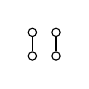
\begin{tikzpicture}
[scale=.3, e/.style={circle,draw,inner sep=0pt,minimum size=3pt}]
\node(a) at (0,1)[e]{};\node(b) at (1,1)[e]{};\node(c) at (0,0)[e]{};\node(d) at (1,0)[e]{};
\draw(a)--(c);\draw(b)--(d);\end{tikzpicture}};
\node(1) at (0.33,-0.33)[e]{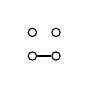
\begin{tikzpicture}
[scale=.3, e/.style={circle,draw,inner sep=0pt,minimum size=3pt}]
\node(a) at (0,1)[e]{};\node(b) at (1,1)[e]{};\node(c) at (0,0)[e]{};\node(d) at (1,0)[e]{};
\draw(c)--(d);\end{tikzpicture}};
\node(0) at (0,-1)[e]{0};
\node at (0,-1.25){\scs 1 ($N_5$)};
\node at (0,1.1)[above]{\begin{tabular}{l}
(1,0,3,2)\\
(1,0,1,0)\end{tabular}};
\node at (0,1.5){};
\draw(3)--(4);
\draw(2)--(4);
\draw(1)--(3);
\draw(0)--(1);
\draw(0)--(2);
\end{tikzpicture}\end{tabular}
\qquad\qquad
\begin{tabular}{l}\begin{tikzpicture}
[scale=2, e/.style={rectangle,draw,rounded corners=3pt}]
\node(4) at (-0.0,1.0)[e]{1};
\node(3) at (0.5,0.0)[e]{\begin{tikzpicture}
[scale=.3, e/.style={circle,draw,inner sep=0pt,minimum size=3pt}]
\node(a) at (0.5,0.87)[e]{};\node(b) at (0,0)[e]{};\node(c) at (1,0)[e]{};
\draw(a)--(b);\end{tikzpicture}};
\node(2) at (0.0,0.0)[e]{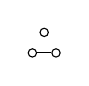
\begin{tikzpicture}
[scale=.3, e/.style={circle,draw,inner sep=0pt,minimum size=3pt}]
\node(a) at (0.5,0.87)[e]{};\node(b) at (0,0)[e]{};\node(c) at (1,0)[e]{};
\draw(b)--(c);\end{tikzpicture}};
\node(1) at (-0.5,0.0)[e]{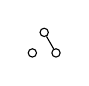
\begin{tikzpicture}
[scale=.3, e/.style={circle,draw,inner sep=0pt,minimum size=3pt}]
\node(a) at (0.5,0.87)[e]{};\node(b) at (0,0)[e]{};\node(c) at (1,0)[e]{};
\draw(a)--(c);\end{tikzpicture}};
\node(0) at (-0.0,-1.0)[e]{0};
\node at (0,-1.25){\scs 2 ($M_3$)};
\node at (0,1.1)[above]{\begin{tabular}{l}
(1,0,3,2)\\
(2,3,0,1)\end{tabular}};
\node at (0,1.5){};
\draw(3)--(4);
\draw(2)--(4);
\draw(1)--(4);
\draw(0)--(1);
\draw(0)--(2);
\draw(0)--(3);
\end{tikzpicture}\end{tabular}
\qquad\qquad
\begin{tabular}{l}\begin{tikzpicture}
[scale=2, e/.style={rectangle,draw,rounded corners=3pt}]
\node(5) at (0,1)[e]{1};
\node(4) at (0.5,0.33)[e]{\begin{tikzpicture}
[scale=.2, e/.style={circle,draw,inner sep=0pt,minimum size=2.5pt}]
\node(a) at (-1,-1)[e]{};\node(b) at (0,-1)[e]{};\node(c) at (1,-1)[e]{};\node(d) at (-1,0)[e]{};
\node(e) at (-1,1)[e]{};\node(f) at (1,0)[e]{};\node(g) at (1,1)[e]{};
\draw(d)--(a)..controls(0,-.4)..(c)--(f);\draw(e)--(g);\end{tikzpicture}};
\node(3) at (-0.5,0.0)[e]{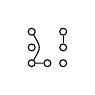
\begin{tikzpicture}
[scale=.2, e/.style={circle,draw,inner sep=0pt,minimum size=2.5pt}]
\node(a) at (-1,-1)[e]{};\node(b) at (0,-1)[e]{};\node(c) at (1,-1)[e]{};\node(d) at (-1,0)[e]{};
\node(e) at (-1,1)[e]{};\node(f) at (1,0)[e]{};\node(g) at (1,1)[e]{};
\draw(e)..controls(-.4,0)..(a)--(b);\draw(f)--(g);\end{tikzpicture}};
\node(2) at (0,0)[e]{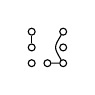
\begin{tikzpicture}
[scale=.2, e/.style={circle,draw,inner sep=0pt,minimum size=2.5pt}]
\node(a) at (-1,-1)[e]{};\node(b) at (0,-1)[e]{};\node(c) at (1,-1)[e]{};\node(d) at (-1,0)[e]{};
\node(e) at (-1,1)[e]{};\node(f) at (1,0)[e]{};\node(g) at (1,1)[e]{};
\draw(b)--(c)..controls(.4,0)..(g);\draw(d)--(e);\end{tikzpicture}};
\node(1) at (0.5,-0.33)[e]{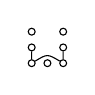
\begin{tikzpicture}
[scale=.2, e/.style={circle,draw,inner sep=0pt,minimum size=2.5pt}]
\node(a) at (-1,-1)[e]{};\node(b) at (0,-1)[e]{};\node(c) at (1,-1)[e]{};\node(d) at (-1,0)[e]{};
\node(e) at (-1,1)[e]{};\node(f) at (1,0)[e]{};\node(g) at (1,1)[e]{};
\draw(d)--(a)..controls(0,-.4)..(c)--(f);\end{tikzpicture}};
\node(0) at (0,-1)[e]{0};
\node at (0,-1.25){\scs 3 $(V_1)$};
\node at (0,1.1)[above]{\begin{tabular}{l}
$p_0=$ (0,1,2,1,2,1,0)\\
$p_1=$ (0,3,4,3,4,3,0)\\
$p_2=$ (6,5,2,5,2,5,6)\\
$p_3=$ (0,1,2,0,0,2,2)\end{tabular}};
\node at (0,1.5){};
\draw(4)--(5);
\draw(3)--(5);
\draw(2)--(5);
\draw(1)--(4);
\draw(0)--(1);
\draw(0)--(2);
\draw(0)--(3);
\end{tikzpicture}\end{tabular}
%\end{document}
%#4 [[1,2,3,4,5,0,7,8,9,10,11,6], #D12 + 2-elt range
%[6,11,10,9,8,7,0,5,4,3,2,1],
%[0,0,0,6,0,0,0,0,6,0,0,0]])
%#5 [[1,0,3,2],[0,0,2,2]])
%#6 [[2,2,1,5,5,4],[3,4,4,0,1,1],[4,5,3,4,5,3]])
%#7 [[1,0,0,4,3,3],[4,5,5,1,2,2],[3,3,4,3,3,4]])
%#8 [[1,2,0,4,5,3],[3,5,4,0,2,1]])
%#9 [[0,0,0,0,0,0,2,1,2,1,3,4,5,3,4,5], 
%[0,0,0,0,0,0,6,7,6,7,10,11,12,10,11,12], 
%[13,14,15,1,9,8,15,14,13,15,1,9,8,8,1,9]]
%#10 No finite algebra known with this congruence lattice
%#11 #algebra from filter-ideal in upper interval of SmallGroup(216,153) found by William Demeo using GAP
%#108 elements (not known to be the smallest)
%#12 [[0,0,3,3,3,6,6,6,0],[0,0,8,8,8,1,1,1,0],[0,5,5,4,0,0,5,4,4],[4,2,2,3,4,4,2,3,3],[5,5,7,7,7,6,6,6,5]])
%#13 [
%( 0, 1, 2, 0, 0, 2, 2, 0, 3, 4, 0, 4, 4, 6, 5, 2, 6, 6, 2), 
%( 0, 1, 2, 3, 4, 5, 6, 0, 1, 2, 4, 5, 6, 0, 1, 2, 3, 4, 6), 
%( 7, 8, 9, 3,10,11,12, 3, 3, 3, 3, 3, 3,11,11,11,11,11,11), 
%(13,14,15,16,17, 5,18,13,16,17,17,16,13, 5, 5, 5, 5, 5, 5),
%( 0, 1, 2, 1, 2, 1, 0, 0, 1, 2, 2, 1, 0, 0, 1, 2, 1, 2, 0)])
%#14 (dual of #15)
%#no explicit small representation known?
%#15 [[1,0,3,2]]
%#16 (dual of #17)
%#no explicit small representation known?
%#17 ((M_3+1)||1)
%#representation from filter-ideal of Sub(A_4)
%[(1,0,3,2,5,4,7,6,9,8,11,10),
%(4,7,5,6,8,11,9,10,0,3,1,2),
%(0,0,0,0,5,5,5,5,10,10,10,10)]
%#18 (dual of #19)
%#no explicit small representation known?
%#19
%#representation found by search in Equ(8) by Peter (smallest)
%[(0,1,1,0,4,5,5,4),
%(0,2,3,1,0,2,3,1),
%(7,6,6,7,3,2,2,3)])
%#20
%#representation found by William Demeo in SmallGroup(216,153)
%#21
%#representation found by Ralph Freese searching through Equ(10)
%#22 (dual of #23)
%#no explicit small representation known?
%#23
%#representation found by searching through Equ(6)
%[(0,1,0,1,4,4), (1,1,3,3,4,5), (3,2,3,2,5,5), (4,1,5,3,4,5)]
%#24 (L_2 in Jonsson-Rival 1979)
%#representation found by searching through Equ(6)
%[(1,1,2,2), (2,3,3,2)]
%#25 (L_1 in Jonsson-Rival 1979)
%[(0, 0, 2, 2, 2), (0, 1, 0, 1, 1), (1, 1, 4, 4, 4), (2, 3, 2, 3, 3)]
%#26 [(1, 0, 3, 2, 0, 2), (4, 4, 5, 5, 1, 3),(0, 0, 0, 0, 1, 1), (3, 5, 3, 5, 3, 3)]
%#27 (4||5)
%#representation from rabbit ears construction applied to #6. |A|=16 (not known to be smallest)
%[
%[ 0, 6, 7, 8, 9,10, 6, 7, 8, 9,10, 0, 6, 8, 9,10], 
%[11,12, 2,13,14,15,12, 2,13,14,15,11,12,13,14,15], 
%[ 0, 1, 2, 3, 4, 5, 0, 0, 0, 0, 0, 2, 2, 2, 2, 2], 
%[ 4, 5, 3, 4, 5, 3, 5, 3, 4, 5, 3, 4, 5, 4, 5, 3], 
%[ 2, 2, 1, 5, 5, 4, 2, 1, 5, 5, 4, 2, 2, 5, 5, 4], 
%[ 3, 4, 4, 0, 1, 1, 4, 4, 0, 1, 1, 3, 4, 0, 1, 1]]
%
%
\qquad\qquad
\begin{tabular}{l}\begin{tikzpicture}
[scale=2, e/.style={rectangle,draw,rounded corners=3pt}]
\node(5) at (0,1)[e]{1};
\node(4) at (0,0.33)[e]{\begin{tikzpicture}
[scale=.2, e/.style={circle,draw,inner sep=0pt,minimum size=3pt}]
\node(a) at (0,1.2)[e]{};\node(b) at (1,1.2)[e]{};\node(c) at (2,1.2)[e]{};\node(d) at (3,1.2)[e]{};
\node(e) at (4,1.2)[e]{};\node(f) at (5,1.2)[e]{};\node(g) at (0,0)[e]{};\node(h) at (1,0)[e]{};
\node(i) at (2,0)[e]{};\node(j) at (3,0)[e]{};\node(k) at (4,0)[e]{};\node(l) at (5,0)[e]{};
\draw(a)--(b)--(c)--(d)--(e)--(f);\draw(g)--(h)--(i)--(j)--(k)--(l);\end{tikzpicture}};
\node(3) at (1,0.33)[e]{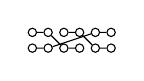
\begin{tikzpicture}
[scale=.2, e/.style={circle,draw,inner sep=0pt,minimum size=3pt}]
\node(a) at (0,1)[e]{};\node(b) at (1,1)[e]{};\node(c) at (2,1)[e]{};\node(d) at (3,1)[e]{};
\node(e) at (4,1)[e]{};\node(f) at (5,1)[e]{};\node(g) at (0,0)[e]{};\node(h) at (1,0)[e]{};
\node(i) at (2,0)[e]{};\node(j) at (3,0)[e]{};\node(k) at (4,0)[e]{};\node(l) at (5,0)[e]{};
\draw(a)--(b)--(i)--(j);\draw(c)--(d)--(k)--(l);\draw(g)--(h)--(e)--(f);\end{tikzpicture}};
\node(2) at (-0.75,0)[e]{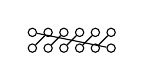
\begin{tikzpicture}
[scale=.2, e/.style={circle,draw,inner sep=0pt,minimum size=3pt}]
\node(a) at (0,1)[e]{};\node(b) at (1,1)[e]{};\node(c) at (2,1)[e]{};\node(d) at (3,1)[e]{};
\node(e) at (4,1)[e]{};\node(f) at (5,1)[e]{};\node(g) at (0,0)[e]{};\node(h) at (1,0)[e]{};
\node(i) at (2,0)[e]{};\node(j) at (3,0)[e]{};\node(k) at (4,0)[e]{};\node(l) at (5,0)[e]{};
\draw(a)--(l);\draw(b)--(g);\draw(c)--(h);\draw(d)--(i);\draw(e)--(j);\draw(f)--(k);\end{tikzpicture}};
\node(1) at (0.5,-0.33)[e]{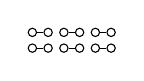
\begin{tikzpicture}
[scale=.2, e/.style={circle,draw,inner sep=0pt,minimum size=3pt}]
\node(a) at (0,1)[e]{};\node(b) at (1,1)[e]{};\node(c) at (2,1)[e]{};\node(d) at (3,1)[e]{};
\node(e) at (4,1)[e]{};\node(f) at (5,1)[e]{};\node(g) at (0,0)[e]{};\node(h) at (1,0)[e]{};
\node(i) at (2,0)[e]{};\node(j) at (3,0)[e]{};\node(k) at (4,0)[e]{};\node(l) at (5,0)[e]{};
\draw(a)--(b);\draw(c)--(d);\draw(e)--(f);\draw(g)--(h);\draw(i)--(j);\draw(k)--(l);\end{tikzpicture}};
\node(0) at (0,-1)[e]{0};
\node at (0,-1.25){\scs 4 $(L_5)$};
\node at (0,1.1)[above]{\begin{tabular}{l}
(1,2,3,4,5,0,7,8,9,10,11,6)\\
(6,11,10,9,8,7,0,5,4,3,2,1)\\
(0,\phantom{1}0,\phantom{1}0,6,0,0,0,0,6,0,0,0)\end{tabular}};
\node at (0,1.5){};
\draw(4)--(5);
\draw(3)--(5);
\draw(2)--(5);
\draw(1)--(3);
\draw(1)--(4);
\draw(0)--(1);
\draw(0)--(2);
\end{tikzpicture}\end{tabular}
\qquad\qquad
\begin{tabular}{l}\begin{tikzpicture}
[scale=2, e/.style={rectangle,draw,rounded corners=3pt}]
\node(5) at (0,1)[e]{1};
\node(4) at (0.2,0.33)[e]{\begin{tikzpicture}
[scale=.3, e/.style={circle,draw,inner sep=0pt,minimum size=3pt}]
\node(a) at (0,1)[e]{};\node(b) at (1,1)[e]{};\node(c) at (0,0)[e]{};\node(d) at (1,0)[e]{};
\draw(a)--(b);\draw(c)--(d);\end{tikzpicture}};
\node(3) at (-0.5,0)[e]{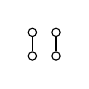
\begin{tikzpicture}
[scale=.3, e/.style={circle,draw,inner sep=0pt,minimum size=3pt}]
\node(a) at (0,1)[e]{};\node(b) at (1,1)[e]{};\node(c) at (0,0)[e]{};\node(d) at (1,0)[e]{};
\draw(a)--(c);\draw(b)--(d);\end{tikzpicture}};
\node(2) at (0.34,-0.33)[e]{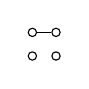
\begin{tikzpicture}
[scale=.3, e/.style={circle,draw,inner sep=0pt,minimum size=3pt}]
\node(a) at (0,1)[e]{};\node(b) at (1,1)[e]{};\node(c) at (0,0)[e]{};\node(d) at (1,0)[e]{};
\draw(a)--(b);\end{tikzpicture}};
\node(1) at (0,-0.33)[e]{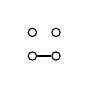
\begin{tikzpicture}
[scale=.3, e/.style={circle,draw,inner sep=0pt,minimum size=3pt}]
\node(a) at (0,1)[e]{};\node(b) at (1,1)[e]{};\node(c) at (0,0)[e]{};\node(d) at (1,0)[e]{};
\draw(c)--(d);\end{tikzpicture}};
\node(0) at (0,-1)[e]{0};
\node at (0,-1.25){\scs 5 $(L_4)$};
\node at (0,1.1)[above]{\begin{tabular}{l}
(1,0,3,2)\\ 
(0,0,2,2)\end{tabular}};
\node at (0,1.5){};
\draw(4)--(5);
\draw(3)--(5);
\draw(2)--(4);
\draw(1)--(4);
\draw(0)--(3);
\draw(0)--(2);
\draw(0)--(1);
\end{tikzpicture}\end{tabular}
\qquad\qquad
\begin{tabular}{l}\begin{tikzpicture}
[scale=2, e/.style={rectangle,draw,rounded corners=3pt}]
\node(5) at (0,1)[e]{1};
\node(4) at (-0.5,0.33)[e]{\begin{tikzpicture}
[scale=.3, e/.style={circle,draw,inner sep=0pt,minimum size=3pt}]
\node(a) at (0,1)[e]{};\node(b) at (1,1)[e]{};\node(c) at (2,1)[e]{};\node(d) at (0,0)[e]{};\node(e) at (1,0)[e]{};\node(f) at (2,0)[e]{};
\draw(a)--(d);\draw(b)--(e);\draw(c)--(f);\end{tikzpicture}};
\node(3) at (0.5,0.33)[e]{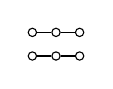
\begin{tikzpicture}
[scale=.3, e/.style={circle,draw,inner sep=0pt,minimum size=3pt}]
\node(a) at (0,1)[e]{};\node(b) at (1,1)[e]{};\node(c) at (2,1)[e]{};\node(d) at (0,0)[e]{};\node(e) at (1,0)[e]{};\node(f) at (2,0)[e]{};
\draw(a)--(b)--(c);\draw(d)--(e)--(f);\end{tikzpicture}};
\node(2) at (-0.5,-0.33)[e]{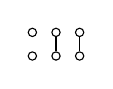
\begin{tikzpicture}
[scale=.3, e/.style={circle,draw,inner sep=0pt,minimum size=3pt}]
\node(a) at (0,1)[e]{};\node(b) at (1,1)[e]{};\node(c) at (2,1)[e]{};\node(d) at (0,0)[e]{};\node(e) at (1,0)[e]{};\node(f) at (2,0)[e]{};
\draw(b)--(e);\draw(c)--(f);\end{tikzpicture}};
\node(1) at (0.5,-0.33)[e]{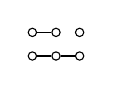
\begin{tikzpicture}
[scale=.3, e/.style={circle,draw,inner sep=0pt,minimum size=3pt}]
\node(a) at (0,1)[e]{};\node(b) at (1,1)[e]{};\node(c) at (2,1)[e]{};\node(d) at (0,0)[e]{};\node(e) at (1,0)[e]{};\node(f) at (2,0)[e]{};
\draw(a)--(b);\draw(d)--(e)--(f);\end{tikzpicture}};
\node(0) at (0,-1)[e]{0};
\node at (0,-1.25){\scs 6};
\node at (0,1.1)[above]{\begin{tabular}{l}
(2,2,1,5,5,4)\\
(3,4,4,0,1,1)\\
(4,5,3,4,5,3)\end{tabular}};
\node at (0,1.5){};
\draw(4)--(5);
\draw(3)--(5);
\draw(2)--(4);
\draw(1)--(3);
\draw(0)--(1);
\draw(0)--(2);
\end{tikzpicture}\end{tabular}
\qquad\qquad
\begin{tabular}{l}\begin{tikzpicture}
[scale=2, e/.style={rectangle,draw,rounded corners=3pt}]
\node(5) at (0,1)[e]{1};
\node(4) at (0.5,0.5)[e]{\begin{tikzpicture}
[scale=.3, e/.style={circle,draw,inner sep=0pt,minimum size=3pt}]
\node(a) at (0,1)[e]{};\node(b) at (1,1)[e]{};\node(c) at (2,1)[e]{};\node(d) at (0,0)[e]{};\node(e) at (1,0)[e]{};\node(f) at (2,0)[e]{};
\draw(a)--(b)--(c);\draw(d)--(e)--(f);\end{tikzpicture}};
\node(3) at (-0.5,0)[e]{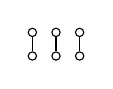
\begin{tikzpicture}
[scale=.3, e/.style={circle,draw,inner sep=0pt,minimum size=3pt}]
\node(a) at (0,1)[e]{};\node(b) at (1,1)[e]{};\node(c) at (2,1)[e]{};\node(d) at (0,0)[e]{};\node(e) at (1,0)[e]{};\node(f) at (2,0)[e]{};
\draw(a)--(d);\draw(b)--(e);\draw(c)--(f);\end{tikzpicture}};
\node(2) at (0.5,0)[e]{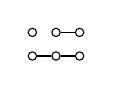
\begin{tikzpicture}
[scale=.3, e/.style={circle,draw,inner sep=0pt,minimum size=3pt}]
\node(a) at (0,1)[e]{};\node(b) at (1,1)[e]{};\node(c) at (2,1)[e]{};\node(d) at (0,0)[e]{};\node(e) at (1,0)[e]{};\node(f) at (2,0)[e]{};
\draw(b)--(c);\draw(d)--(e)--(f);\end{tikzpicture}};
\node(1) at (0.5,-0.5)[e]{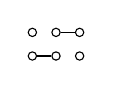
\begin{tikzpicture}
[scale=.3, e/.style={circle,draw,inner sep=0pt,minimum size=3pt}]
\node(a) at (0,1)[e]{};\node(b) at (1,1)[e]{};\node(c) at (2,1)[e]{};\node(d) at (0,0)[e]{};\node(e) at (1,0)[e]{};\node(f) at (2,0)[e]{};
\draw(b)--(c);\draw(d)--(e);\end{tikzpicture}};
\node(0) at (0,-1)[e]{0};
\node at (0,-1.25){\scs 7};
\node at (0,1.1)[above]{\begin{tabular}{l}
(1,0,0,4,3,3)\\
(4,5,5,1,2,2)\\
(3,3,4,3,3,4)\end{tabular}};
\node at (0,1.5){};
\draw(4)--(5);
\draw(3)--(5);
\draw(2)--(4);
\draw(1)--(2);
\draw(0)--(1);
\draw(0)--(3);
\end{tikzpicture}\end{tabular}
\qquad\qquad
\begin{tabular}{l}\begin{tikzpicture}
[scale=2, e/.style={rectangle,draw,rounded corners=3pt}]
\node(5) at (0,1)[e]{1};
\node(4) at (-1,0.0)[e]{\begin{tikzpicture}
[scale=.3, e/.style={circle,draw,inner sep=0pt,minimum size=3pt}]
\node(a) at (0,1)[e]{};\node(b) at (1,1)[e]{};\node(c) at (2,1)[e]{};\node(d) at (0,0)[e]{};\node(e) at (1,0)[e]{};\node(f) at (2,0)[e]{};
\draw(a)--(b)--(c);\draw(d)--(e)--(f);\end{tikzpicture}};
\node(3) at (-.33,0)[e]{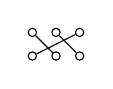
\begin{tikzpicture}
[scale=.3, e/.style={circle,draw,inner sep=0pt,minimum size=3pt}]
\node(a) at (0,1)[e]{};\node(b) at (1,1)[e]{};\node(c) at (2,1)[e]{};\node(d) at (0,0)[e]{};\node(e) at (1,0)[e]{};\node(f) at (2,0)[e]{};
\draw(a)--(e);\draw(b)--(f);\draw(c)--(d);\end{tikzpicture}};
\node(2) at (0.33,0)[e]{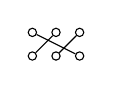
\begin{tikzpicture}
[scale=.3, e/.style={circle,draw,inner sep=0pt,minimum size=3pt}]
\node(a) at (0,1)[e]{};\node(b) at (1,1)[e]{};\node(c) at (2,1)[e]{};\node(d) at (0,0)[e]{};\node(e) at (1,0)[e]{};\node(f) at (2,0)[e]{};
\draw(a)--(f);\draw(b)--(d);\draw(c)--(e);\end{tikzpicture}};
\node(1) at (1,0)[e]{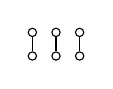
\begin{tikzpicture}
[scale=.3, e/.style={circle,draw,inner sep=0pt,minimum size=3pt}]
\node(a) at (0,1)[e]{};\node(b) at (1,1)[e]{};\node(c) at (2,1)[e]{};\node(d) at (0,0)[e]{};\node(e) at (1,0)[e]{};\node(f) at (2,0)[e]{};
\draw(a)--(d);\draw(b)--(e);\draw(c)--(f);\end{tikzpicture}};
\node(0) at (0,-1)[e]{0};
\node at (0,-1.25){\scs 8 $(M_4)$};
\node at (0,1.1)[above]{\begin{tabular}{l}
(1,2,0,4,5,3)\\
(3,5,4,0,2,1)\end{tabular}};
\node at (0,1.5){};
\draw(4)--(5);
\draw(3)--(5);
\draw(2)--(5);
\draw(1)--(5);
\draw(0)--(1);
\draw(0)--(2);
\draw(0)--(3);
\draw(0)--(4);
\end{tikzpicture}\end{tabular}
\begin{tabular}{l}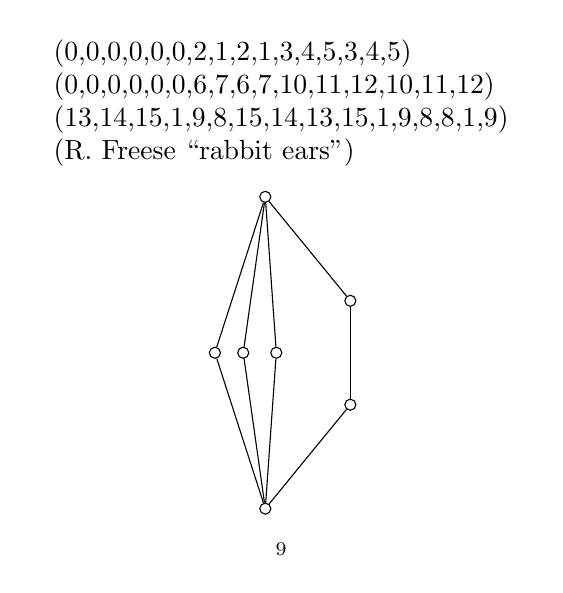
\begin{tikzpicture}
[scale=2, e/.style={circle,draw,inner sep=0pt,minimum size=4pt}]
\node(6) at (-0.1,0.99)[e]{};
\node(5) at (0.44,0.33)[e]{};
\node(4) at (-0.24,0.0)[e]{};
\node(3) at (-0.42,0.0)[e]{};
\node(2) at (-0.03,0.0)[e]{};
\node(1) at (0.44,-0.33)[e]{};
\node(0) at (-0.1,-0.99)[e]{};
\node at (0,-1.25){\scs 9};
\node at (0,1.1)[above]{\begin{tabular}{l}
(0,0,0,0,0,0,2,1,2,1,3,4,5,3,4,5)\\
(0,0,0,0,0,0,6,7,6,7,10,11,12,10,11,12)\\ 
(13,14,15,1,9,8,15,14,13,15,1,9,8,8,1,9)\\
(R. Freese ``rabbit ears'')
\end{tabular}};
\node at (0,1.5){};
\draw(5)--(6);
\draw(4)--(6);
\draw(3)--(6);
\draw(2)--(6);
\draw(1)--(5);
\draw(0)--(1);
\draw(0)--(2);
\draw(0)--(3);
\draw(0)--(4);
\end{tikzpicture}\end{tabular}
\begin{tabular}{l}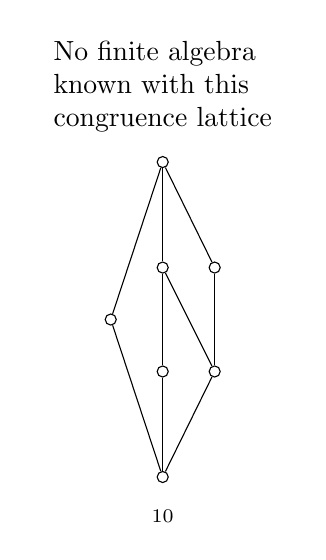
\begin{tikzpicture}
[scale=2, e/.style={circle,draw,inner sep=0pt,minimum size=4pt}]
\node(6) at (0,1)[e]{};
\node(5) at (0,0.33)[e]{};
\node(4) at (0.33,0.33)[e]{};
\node(3) at (-0.33,0.0)[e]{};
\node(2) at (0,-0.33)[e]{};
\node(1) at (0.33,-0.33)[e]{};
\node(0) at (0,-1)[e]{};
\node at (0,-1.25){\scs 10};
\node at (0,1.1)[above]{\begin{tabular}{l}
No finite algebra\\
known with this\\
congruence lattice\end{tabular}};
\node at (0,1.5){};
\draw(5)--(6);
\draw(4)--(6);
\draw(3)--(6);
\draw(2)--(5);
\draw(1)--(4);
\draw(1)--(5);
\draw(0)--(1);
\draw(0)--(2);
\draw(0)--(3);
\end{tikzpicture}\end{tabular}
\begin{tabular}{l}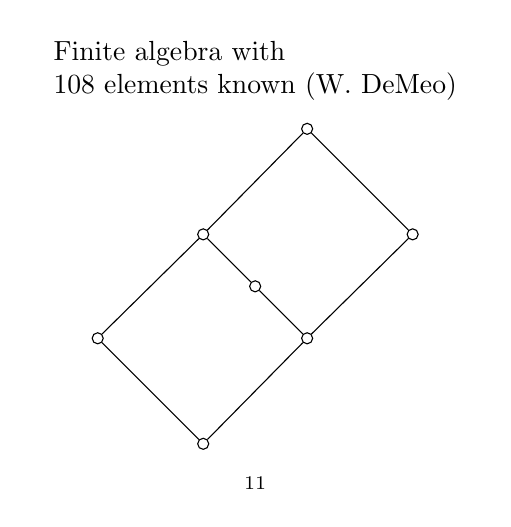
\begin{tikzpicture}
[scale=2, e/.style={circle,draw,inner sep=0pt,minimum size=4pt}]
\node(6) at (0.33,1)[e]{};
\node(5) at (-0.33,0.33)[e]{};
\node(4) at (1,0.33)[e]{};
\node(3) at (0,0)[e]{};
\node(2) at (-1,-0.33)[e]{};
\node(1) at (0.33,-0.33)[e]{};
\node(0) at (-0.33,-1)[e]{};
\node at (0,-1.25){\scs 11};
\node at (0,1.1)[above]{\begin{tabular}{l}
Finite algebra with\\
108 elements known (W. DeMeo)\end{tabular}};
\node at (0,1.5){};
\draw(5)--(6);
\draw(4)--(6);
\draw(3)--(5);
\draw(2)--(5);
\draw(1)--(3);
\draw(1)--(4);
\draw(0)--(1);
\draw(0)--(2);
\end{tikzpicture}\end{tabular}
\begin{tabular}{l}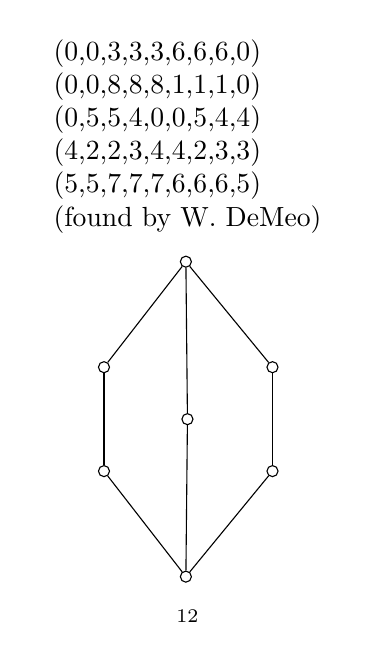
\begin{tikzpicture}
[scale=2, e/.style={circle,draw,inner sep=0pt,minimum size=4pt}]
\node(6) at (-0.01,1.0)[e]{};
\node(5) at (0.54,0.33)[e]{};
\node(4) at (-0.53,0.33)[e]{};
\node(3) at (0.0,0.0)[e]{};
\node(2) at (0.54,-0.33)[e]{};
\node(1) at (-0.53,-0.33)[e]{};
\node(0) at (-0.01,-1.0)[e]{};
\node at (0,-1.25){\scs 12 };
\node at (0,1.1)[above]{\begin{tabular}{l}
(0,0,3,3,3,6,6,6,0)\\
(0,0,8,8,8,1,1,1,0)\\
(0,5,5,4,0,0,5,4,4)\\
(4,2,2,3,4,4,2,3,3)\\
(5,5,7,7,7,6,6,6,5)\\
(found by W. DeMeo)\end{tabular}};
\node at (0,1.5){};
\draw(5)--(6);
\draw(4)--(6);
\draw(3)--(6);
\draw(2)--(5);
\draw(1)--(4);
\draw(0)--(1);
\draw(0)--(2);
\draw(0)--(3);
\end{tikzpicture}\end{tabular}
\begin{tabular}{l}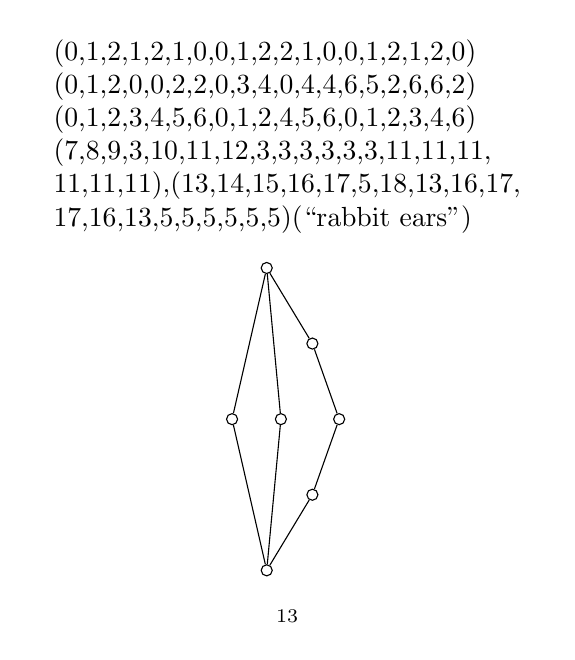
\begin{tikzpicture}
[scale=2, e/.style={circle,draw,inner sep=0pt,minimum size=4pt}]
\node(6) at (-0.13,0.96)[e]{};
\node(5) at (0.16,0.48)[e]{};
\node(4) at (-0.04,0.0)[e]{};
\node(3) at (-0.35,0.0)[e]{};
\node(2) at (0.33,0.0)[e]{};
\node(1) at (0.16,-0.48)[e]{};
\node(0) at (-0.13,-0.96)[e]{};
\node at (0,-1.25){\scs 13 };
\node at (0,1.1)[above]{\begin{tabular}{l}
(0,1,2,1,2,1,0,0,1,2,2,1,0,0,1,2,1,2,0)\\
(0,1,2,0,0,2,2,0,3,4,0,4,4,6,5,2,6,6,2)\\
(0,1,2,3,4,5,6,0,1,2,4,5,6,0,1,2,3,4,6)\\
(7,8,9,3,10,11,12,3,3,3,3,3,3,11,11,11,\\
11,11,11),(13,14,15,16,17,5,18,13,16,17,\\
17,16,13,5,5,5,5,5,5)(``rabbit ears'')\end{tabular}};
\node at (0,1.5){};
\draw(5)--(6);
\draw(4)--(6);
\draw(3)--(6);
\draw(2)--(5);
\draw(1)--(2);
\draw(0)--(1);
\draw(0)--(3);
\draw(0)--(4);
\end{tikzpicture}\end{tabular}
\begin{tabular}{l}\begin{tikzpicture}
[scale=2, e/.style={circle,draw,inner sep=0pt,minimum size=4pt}]
\node(6) at (0,1)[e]{};
\node(5) at (-0.39,0.27)[e]{};
\node(4) at (-0.09,0.27)[e]{};
\node(3) at (0.38,-0.05)[e]{};
\node(2) at (0.16,-0.05)[e]{};
\node(1) at (-0.26,-0.36)[e]{};
\node(0) at (0,-1)[e]{};
\node at (0,-1.25){\scs 14};
\node at (0,1.1)[above]{\begin{tabular}{l}
Upper interval in Sub$(A_6)$\\
algebra of size 90 (W. DeMeo)\end{tabular}};
\node at (0,1.5){};
\draw(5)--(6);
\draw(4)--(6);
\draw(3)--(6);
\draw(2)--(6);
\draw(1)--(4);
\draw(1)--(5);
\draw(0)--(1);
\draw(0)--(2);
\draw(0)--(3);
\end{tikzpicture}\end{tabular}
\begin{tabular}{l}\begin{tikzpicture}
[scale=2, e/.style={circle,draw,inner sep=0pt,minimum size=4pt}]
\node(6) at (0,1)[e]{};
\node(5) at (0.26,0.36)[e]{};
\node(4) at (-0.16,0.05)[e]{};
\node(3) at (-0.38,0.05)[e]{};
\node(2) at (0.08,-0.27)[e]{};
\node(1) at (0.39,-0.27)[e]{};
\node(0) at (0,-1)[e]{};
\node at (0,-1.25){\scs 15};
\node at (0,1.1)[above]{\begin{tabular}{l}
(1,0,3,2)\end{tabular}};
\node at (0,1.5){};
\draw(5)--(6);
\draw(4)--(6);
\draw(3)--(6);
\draw(2)--(5);
\draw(1)--(5);
\draw(0)--(4);
\draw(0)--(3);
\draw(0)--(2);
\draw(0)--(1);
\end{tikzpicture}\end{tabular}
\begin{tabular}{l}\begin{tikzpicture}
[scale=2, e/.style={circle,draw,inner sep=0pt,minimum size=4pt}]
\node(6) at (0,1)[e]{};
\node(5) at (0.12,0.22)[e]{};
\node(4) at (-0.37,0.22)[e]{};
\node(3) at (-0.13,0.22)[e]{};
\node(2) at (0.34,-0.09)[e]{};
\node(1) at (-0.15,-0.39)[e]{};
\node(0) at (0,-1)[e]{};
\node at (0,-1.25){\scs 16};
\node at (0,1.1)[above]{\begin{tabular}{l}
Upper interval in Sub$(C_2.A_6)$\\
algebra of size 180 (W. DeMeo)\end{tabular}};
\node at (0,1.5){};
\draw(5)--(6);
\draw(4)--(6);
\draw(3)--(6);
\draw(2)--(6);
\draw(1)--(3);
\draw(1)--(4);
\draw(1)--(5);
\draw(0)--(1);
\draw(0)--(2);
\end{tikzpicture}\end{tabular}
\begin{tabular}{l}\begin{tikzpicture}
[scale=2, e/.style={circle,draw,inner sep=0pt,minimum size=4pt}]
\node(6) at (0,1.0)[e]{};
\node(5) at (-0.14,0.39)[e]{};
\node(4) at (0.34,0.09)[e]{};
\node(3) at (0.12,-0.22)[e]{};
\node(2) at (-0.11,-0.22)[e]{};
\node(1) at (-0.37,-0.22)[e]{};
\node(0) at (0,-1)[e]{};
\node at (0,-1.25){\scs 17};
\node at (0,1.1)[above]{\begin{tabular}{l}
(1,0,3,2,5,4,7,6,9,8,11,10)\\
(4,7,5,6,8,11,9,10,0,3,1,2)\\
(0,0,0,0,5,5,5,5,10,10,10,10)\\
(W. Demeo, filter-ideal in Sub$(A_4)$)\end{tabular}};
\node at (0,1.5){};
\draw(5)--(6);
\draw(4)--(6);
\draw(3)--(5);
\draw(2)--(5);
\draw(1)--(5);
\draw(0)--(4);
\draw(0)--(3);
\draw(0)--(2);
\draw(0)--(1);
\end{tikzpicture}\end{tabular}
\begin{tabular}{l}\begin{tikzpicture}
[scale=2, e/.style={circle,draw,inner sep=0pt,minimum size=4pt}]
\node(6) at (0.01,0.91)[e]{};
\node(5) at (0.35,0.27)[e]{};
\node(4) at (-0.43,0.27)[e]{};
\node(3) at (-0.03,0.27)[e]{};
\node(2) at (0.34,-0.36)[e]{};
\node(1) at (-0.25,-0.36)[e]{};
\node(0) at (0.01,-1.0)[e]{};
\node at (0,-1.25){\scs 18};
\node at (0,1.1)[above]{\begin{tabular}{l}
Dual of 19, no explicit\\
small representation known?\end{tabular}};
\node at (0,1.5){};
\draw(5)--(6);
\draw(4)--(6);
\draw(3)--(6);
\draw(2)--(5);
\draw(1)--(3);
\draw(1)--(4);
\draw(0)--(1);
\draw(0)--(2);
\end{tikzpicture}\end{tabular}
\begin{tabular}{l}\begin{tikzpicture}
[scale=2, e/.style={circle,draw,inner sep=0pt,minimum size=4pt}]
\node(6) at (-0.01,1.0)[e]{};
\node(5) at (0.26,0.36)[e]{};
\node(4) at (-0.35,0.36)[e]{};
\node(3) at (0.44,-0.27)[e]{};
\node(2) at (0.04,-0.27)[e]{};
\node(1) at (-0.36,-0.27)[e]{};
\node(0) at (-0.01,-0.91)[e]{};
\node at (0,-1.25){\scs 19};
\node at (0,1.1)[above]{\begin{tabular}{l}
(0,1,1,0,4,5,5,4)\\
(0,2,3,1,0,2,3,1)\\
(7,6,6,7,3,2,2,3)\\
(P. Jipsen, search in Equ(8))
\end{tabular}};
\node at (0,1.5){};
\draw(5)--(6);
\draw(4)--(6);
\draw(3)--(5);
\draw(2)--(5);
\draw(1)--(4);
\draw(0)--(3);
\draw(0)--(2);
\draw(0)--(1);
\end{tikzpicture}\end{tabular}
\begin{tabular}{l}\begin{tikzpicture}
[scale=2, e/.style={circle,draw,inner sep=0pt,minimum size=4pt}]
\node(6) at (-0.24,0.9)[e]{};
\node(5) at (0.28,0.43)[e]{};
\node(4) at (-0.07,0.2)[e]{};
\node(3) at (-0.45,-0.03)[e]{};
\node(2) at (0.57,-0.03)[e]{};
\node(1) at (0.16,-0.5)[e]{};
\node(0) at (-0.24,-0.97)[e]{};
\node at (0,-1.25){\scs 20};
\node at (0,1.1)[above]{\begin{tabular}{l}
(W. DeMeo in GAP \\
SmallGroup(216,153))\end{tabular}};
\node at (0,1.5){};
\draw(5)--(6);
\draw(4)--(6);
\draw(3)--(6);
\draw(2)--(5);
\draw(1)--(2);
\draw(1)--(4);
\draw(0)--(1);
\draw(0)--(3);
\end{tikzpicture}\end{tabular}
\begin{tabular}{l}\begin{tikzpicture}
[scale=2, e/.style={circle,draw,inner sep=0pt,minimum size=4pt}]
\node(6) at (0.25,0.97)[e]{};
\node(5) at (-0.15,0.5)[e]{};
\node(4) at (-0.59,0.03)[e]{};
\node(3) at (0.46,0.03)[e]{};
\node(2) at (0.1,-0.2)[e]{};
\node(1) at (-0.31,-0.43)[e]{};
\node(0) at (0.25,-0.9)[e]{};
\node at (0,-1.25){\scs 21};
\node at (0,1.1)[above]{\begin{tabular}{l}
(3,3,4,8,8,2,2,3,4)\\
(0,0,6,1,1,0,0,5,6)\\
(4,5,5,7,8,8,7,4,4)\\
(R. Freese, in Equ(9))\end{tabular}};
\node at (0,1.5){};
\draw(5)--(6);
\draw(4)--(5);
\draw(3)--(6);
\draw(2)--(5);
\draw(1)--(4);
\draw(0)--(3);
\draw(0)--(2);
\draw(0)--(1);
\end{tikzpicture}\end{tabular}
\begin{tabular}{l}\begin{tikzpicture}
[scale=2, e/.style={circle,draw,inner sep=0pt,minimum size=4pt}]
\node(6) at (0,1)[e]{};
\node(5) at (-0.33,0.5)[e]{};
\node(4) at (0,0.5)[e]{};
\node(3) at (0.33,0)[e]{};
\node(2) at (-0.33,0)[e]{};
\node(1) at (-0.33,-0.5)[e]{};
\node(0) at (0,-1)[e]{};
\node at (0,-1.25){\scs 22};
\node at (0,1.1)[above]{\begin{tabular}{l}
Dual of 23, no\\
explicit small\\
representation\\
known?\end{tabular}};
\node at (0,1.5){};
\draw(5)--(6);
\draw(4)--(6);
\draw(3)--(6);
\draw(2)--(4);
\draw(2)--(5);
\draw(1)--(2);
\draw(0)--(1);
\draw(0)--(3);
\end{tikzpicture}\end{tabular}
\begin{tabular}{l}\begin{tikzpicture}
[scale=2, e/.style={circle,draw,inner sep=0pt,minimum size=4pt}]
\node(6) at (0,1)[e]{};
\node(5) at (-0.33,0.5)[e]{};
\node(4) at (-0.33,0)[e]{};
\node(3) at (0.33,0)[e]{};
\node(2) at (-0.33,-0.5)[e]{};
\node(1) at (0,-0.5)[e]{};
\node(0) at (0,-1)[e]{};
\node at (0,-1.25){\scs 23};
\node at (0,1.1)[above]{\begin{tabular}{l}
(0,1,0,1,4,4)\\
(1,1,3,3,4,5)\\
(3,2,3,2,5,5)\\
(4,1,5,3,4,5)
\end{tabular}};
\node at (0,1.5){};
\draw(5)--(6);
\draw(4)--(5);
\draw(3)--(6);
\draw(2)--(4);
\draw(1)--(4);
\draw(0)--(3);
\draw(0)--(2);
\draw(0)--(1);
\end{tikzpicture}\end{tabular}
\begin{tabular}{l}\begin{tikzpicture}
[scale=2, e/.style={circle,draw,inner sep=0pt,minimum size=4pt}]
\node(6) at (-0.0,0.91)[e]{};
\node(5) at (0.0,0.27)[e]{};
\node(4) at (0.5,0.27)[e]{};
\node(3) at (-0.5,0.27)[e]{};
\node(2) at (0.33,-0.36)[e]{};
\node(1) at (-0.33,-0.36)[e]{};
\node(0) at (-0.0,-1.0)[e]{};
\node at (0,-1.25){\scs 24 ($L_2$)};
\node at (0,1.1)[above]{\begin{tabular}{l}
(1,1,2,2)\\
(2,3,3,2)\end{tabular}};
\node at (0,1.5){};
\draw(5)--(6);
\draw(4)--(6);
\draw(3)--(6);
\draw(2)--(4);
\draw(2)--(5);
\draw(1)--(3);
\draw(1)--(5);
\draw(0)--(1);
\draw(0)--(2);
\end{tikzpicture}\end{tabular}
\begin{tabular}{l}\begin{tikzpicture}
[scale=2, e/.style={circle,draw,inner sep=0pt,minimum size=4pt}]
\node(6) at (0.01,1.0)[e]{};
\node(5) at (-0.34,0.36)[e]{};
\node(4) at (0.33,0.36)[e]{};
\node(3) at (-0.5,-0.27)[e]{};
\node(2) at (0.5,-0.27)[e]{};
\node(1) at (-0.01,-0.27)[e]{};
\node(0) at (0.01,-0.91)[e]{};
\node at (0,-1.25){\scs 25 ($L_1$)};
\node at (0,1.1)[above]{\begin{tabular}{l}
(0,0,2,2,2)\\
(0,1,0,1,1)\\
(1,1,4,4,4)\\
(2,3,2,3,3)\end{tabular}};
\node at (0,1.5){};
\draw(5)--(6);
\draw(4)--(6);
\draw(3)--(5);
\draw(2)--(4);
\draw(1)--(5);
\draw(1)--(4);
\draw(0)--(3);
\draw(0)--(2);
\draw(0)--(1);
\end{tikzpicture}\end{tabular}
\begin{tabular}{l}\begin{tikzpicture}
[scale=2, e/.style={circle,draw,inner sep=0pt,minimum size=4pt}]
\node(6) at (-0.25,0.94)[e]{};
\node(5) at (0.14,0.47)[e]{};
\node(4) at (-0.4,0.0)[e]{};
\node(3) at (0.11,0.0)[e]{};
\node(2) at (0.51,0.0)[e]{};
\node(1) at (0.14,-0.47)[e]{};
\node(0) at (-0.25,-0.94)[e]{};
\node at (0,-1.25){\scs 26};
\node at (0,1.1)[above]{\begin{tabular}{l}
(1,0,3,2,0,2)\\
(4,4,5,5,1,3)\\
(0,0,0,0,1,1)\\
(3,5,3,5,3,3)\end{tabular}};
\node at (0,1.5){};
\draw(5)--(6);
\draw(4)--(6);
\draw(3)--(5);
\draw(2)--(5);
\draw(1)--(2);
\draw(1)--(3);
\draw(0)--(1);
\draw(0)--(4);
\end{tikzpicture}\end{tabular}
\begin{tabular}{l}\begin{tikzpicture}
[scale=2, e/.style={circle,draw,inner sep=0pt,minimum size=4pt}]
\node(6) at (0,1)[e]{};
\node(5) at (0.33,0.5)[e]{};
\node(4) at (-0.33,0.25)[e]{};
\node(3) at (0.33,0.0)[e]{};
\node(2) at (-0.33,-0.25)[e]{};
\node(1) at (0.33,-0.5)[e]{};
\node(0) at (0,-1)[e]{};
\node at (0,-1.25){\scs 27};
\node at (0,1.1)[above]{\begin{tabular}{l}
(0,1,2,3,4,5,0,0,0,0,0,2,2,2,2,2)\\
(4,5,3,4,5,3,5,3,4,5,3,4,5,4,5,3)\\
(2,2,1,5,5,4,2,1,5,5,4,2,2,5,5,4)\\
(3,4,4,0,1,1,4,4,0,1,1,3,4,0,1,1)\\
(0,6,7,8,9,10,6,7,8,9,10,0,6,8,9,10)\\
(11,12,2,13,14,15,12,2,13,14,15,\\
11,12,13,14,15) (``rabbit ears'')
\end{tabular}};
\node at (0,1.5){};
\draw(5)--(6);
\draw(4)--(6);
\draw(3)--(5);
\draw(2)--(4);
\draw(1)--(3);
\draw(0)--(1);
\draw(0)--(2);
\end{tikzpicture}\end{tabular}
\begin{tabular}{l}\begin{tikzpicture}
[scale=2, e/.style={circle,draw,inner sep=0pt,minimum size=4pt}]
\node(6) at (0,1)[e]{};
\node(5) at (0.33,0.6)[e]{};
\node(4) at (-0.33,0)[e]{};
\node(3) at (0.33,0.2)[e]{};
\node(2) at (0.33,-0.2)[e]{};
\node(1) at (0.33,-0.6)[e]{};
\node(0) at (0,-1)[e]{};
\node at (0,-1.25){\scs 28};
\node at (0,1.1)[above]{\begin{tabular}{l}
(0,1,2,3,4,5,0,0,0,0,0,2,2,2,2,2)\\
(3,3,4,3,3,4,3,4,3,3,4,3,3,3,3,4)\\
(1,0,0,4,3,3,0,0,4,3,3,1,0,4,3,3)\\
(4,5,5,1,2,2,5,5,1,2,2,4,5,1,2,2)\\
(0,6,7,8,9,10,6,7,8,9,10,0,6,8,9,10)\\
(11,12,2,13,14,15,12,2,13,14,15,\\
11,12,13,14,15) (``rabbit ears'')
\end{tabular}};
\node at (0,1.5){};
\draw(5)--(6);
\draw(4)--(6);
\draw(3)--(5);
\draw(2)--(3);
\draw(1)--(2);
\draw(0)--(1);
\draw(0)--(4);
\end{tikzpicture}\end{tabular}
\begin{tabular}{l}\begin{tikzpicture}
[scale=2, e/.style={circle,draw,inner sep=0pt,minimum size=4pt}]
\node(6) at (-0.19,0.98)[e]{};
\node(5) at (0.38,0.49)[e]{};
\node(4) at (-0.25,0.25)[e]{};
\node(3) at (0.63,0.0)[e]{};
\node(2) at (-0.52,-0.25)[e]{};
\node(1) at (0.15,-0.49)[e]{};
\node(0) at (-0.19,-0.98)[e]{};
\node at (0,-1.25){\scs 29};
\node at (0,1.1)[above]{\begin{tabular}{l}
(1,0,3,2,2)\\
(2,4,2,4,3)\end{tabular}};
\node at (0,1.5){};
\draw(5)--(6);
\draw(4)--(6);
\draw(3)--(5);
\draw(2)--(4);
\draw(1)--(3);
\draw(1)--(4);
\draw(0)--(1);
\draw(0)--(2);
\end{tikzpicture}\end{tabular}
\begin{tabular}{l}\begin{tikzpicture}
[scale=2, e/.style={circle,draw,inner sep=0pt,minimum size=4pt}]
\node(6) at (-0.19,0.98)[e]{};
\node(5) at (0.15,0.49)[e]{};
\node(4) at (-0.52,0.25)[e]{};
\node(3) at (0.63,0.0)[e]{};
\node(2) at (-0.25,-0.25)[e]{};
\node(1) at (0.38,-0.49)[e]{};
\node(0) at (-0.19,-0.98)[e]{};
\node at (0,-1.25){\scs 30};
\node at (0,1.1)[above]{\begin{tabular}{l}
(0,3,4,3,4)\\
(2,2,1,4,3)\end{tabular}};
\node at (0,1.5){};
\draw(5)--(6);
\draw(4)--(6);
\draw(3)--(5);
\draw(2)--(5);
\draw(2)--(4);
\draw(1)--(3);
\draw(0)--(2);
\draw(0)--(1);
\end{tikzpicture}\end{tabular}
\begin{tabular}{l}\begin{tikzpicture}
[scale=2, e/.style={circle,draw,inner sep=0pt,minimum size=4pt}]
\node(6) at (0.09,0.99)[e]{};
\node(5) at (-0.3,0.51)[e]{};
\node(4) at (0.43,0.27)[e]{};
\node(3) at (-0.21,0.03)[e]{};
\node(2) at (-0.37,-0.45)[e]{};
\node(1) at (0.27,-0.45)[e]{};
\node(0) at (0.09,-0.93)[e]{};
\node at (0,-1.25){\scs 31};
\node at (0,1.1)[above]{\begin{tabular}{l}
(0,1,1,0,0)\\
(1,1,2,2,2)\\
(3,2,2,4,4)\end{tabular}};
\node at (0,1.5){};
\draw(5)--(6);
\draw(4)--(6);
\draw(3)--(5);
\draw(2)--(3);
\draw(1)--(3);
\draw(1)--(4);
\draw(0)--(1);
\draw(0)--(2);
\end{tikzpicture}\end{tabular}
\begin{tabular}{l}\begin{tikzpicture}
[scale=2, e/.style={circle,draw,inner sep=0pt,minimum size=4pt}]
\node(6) at (0.09,0.93)[e]{};
\node(5) at (0.28,0.45)[e]{};
\node(4) at (-0.37,0.45)[e]{};
\node(3) at (-0.2,-0.03)[e]{};
\node(2) at (0.44,-0.27)[e]{};
\node(1) at (-0.32,-0.52)[e]{};
\node(0) at (0.09,-1.0)[e]{};
\node at (0,-1.25){\scs 32};
\node at (0,1.1)[above]{\begin{tabular}{l}
(0,1,1,3,3)\\
(1,2,2,4,4)\\
(3,3,4,3,4)
\end{tabular}};
\node at (0,1.5){};
\draw(5)--(6);
\draw(4)--(6);
\draw(3)--(5);
\draw(3)--(4);
\draw(2)--(5);
\draw(1)--(3);
\draw(0)--(2);
\draw(0)--(1);
\end{tikzpicture}\end{tabular}
\begin{tabular}{l}\begin{tikzpicture}
[scale=2, e/.style={circle,draw,inner sep=0pt,minimum size=4pt}]
\node(6) at (0.0,1.0)[e]{};
\node(5) at (-0.41,0.0)[e]{};
\node(4) at (0.25,0.0)[e]{};
\node(3) at (0.0,0.0)[e]{};
\node(2) at (-0.25,0.0)[e]{};
\node(1) at (0.41,0.0)[e]{};
\node(0) at (0.0,-1.0)[e]{};
\node at (0,-1.25){\scs 33 $(M_5)$};
\node at (0,1.1)[above]{\begin{tabular}{l}
(1,3,2,0,9,11,10,8,13,15,14,12,5,7,6,4)\\
(11,8,10,9,7,4,6,5,15,12,14,13,3,0,2,1)\\
(14,15,12,13,10,11,8,9,6,7,4,5,2,3,0,1)\end{tabular}};
\node at (0,1.5){};
\draw(5)--(6);
\draw(4)--(6);
\draw(3)--(6);
\draw(2)--(6);
\draw(1)--(6);
\draw(0)--(1);
\draw(0)--(2);
\draw(0)--(3);
\draw(0)--(4);
\draw(0)--(5);
\end{tikzpicture}\end{tabular}
\begin{tabular}{l}\begin{tikzpicture}
[scale=2, e/.style={circle,draw,inner sep=0pt,minimum size=4pt}]
\node(6) at (0.0,0.91)[e]{};
\node(5) at (0.24,0.27)[e]{};
\node(4) at (-0.42,0.27)[e]{};
\node(3) at (-0.08,0.27)[e]{};
\node(2) at (0.39,-0.36)[e]{};
\node(1) at (-0.13,-0.36)[e]{};
\node(0) at (0.0,-1.0)[e]{};
\node at (0,-1.25){\scs 34};
\node at (0,1.1)[above]{\begin{tabular}{l}
(0,1,3,2)\end{tabular}};
\node at (0,1.5){};
\draw(5)--(6);
\draw(4)--(6);
\draw(3)--(6);
\draw(2)--(5);
\draw(1)--(3);
\draw(1)--(4);
\draw(1)--(5);
\draw(0)--(1);
\draw(0)--(2);
\end{tikzpicture}\end{tabular}
\begin{tabular}{l}\begin{tikzpicture}
[scale=2, e/.style={circle,draw,inner sep=0pt,minimum size=4pt}]
\node(6) at (0.01,1.0)[e]{};
\node(5) at (-0.14,0.36)[e]{};
\node(4) at (0.4,0.36)[e]{};
\node(3) at (-0.41,-0.27)[e]{};
\node(2) at (-0.1,-0.27)[e]{};
\node(1) at (0.24,-0.27)[e]{};
\node(0) at (0.01,-0.91)[e]{};
\node at (0,-1.25){\scs 35};
\node at (0,1.1)[above]{\begin{tabular}{l}
(1,1,2,3)\\
(2,3,3,3)\end{tabular}};
\node at (0,1.5){};
\draw(5)--(6);
\draw(4)--(6);
\draw(3)--(5);
\draw(2)--(5);
\draw(1)--(5);
\draw(1)--(4);
\draw(0)--(3);
\draw(0)--(2);
\draw(0)--(1);
\end{tikzpicture}\end{tabular}
%\end{document}

  (include all major inputs in one file)
%% -- Begin conglattices7.tex file insertion -------------------------------

Distributive lattices and lattices that are ordinal sums of smaller lattices are omitted.
The base set of each algebra is $\{0,1,\dots,n-1\}$, and each unary operation is
specified by a vector of values of these elements.  Algebras of size less than
$11$ are known to be minimal-size algebras that produce the corresponding
congruence lattice. The algebra for 33 $(M_5)$ is also known to be minimal in
size. Currently only one of the lattices (10) is not known to be the congruence
lattice of a finite algebra. 

%Thirteen of the 35 lattices below are subdirectly reducible (specifically: 6, 7,12, 13, 26, 27, 28, 29, 30, 31, 32, 34, 35). 
\scriptsize

\begin{tabular}{l}\begin{tikzpicture}
    [scale=1.2, e/.style={circle,draw,inner sep=0pt,minimum size=5pt}]
\node(4) at (0,1)[e]{};
\node(3) at (0.33,0.33){$1\ 2|3\ 4$};
\node(2) at (-0.5,0.0){$1\ 3|2\ 4$};
\node(1) at (0.33,-0.33){$1|2|3\ 4$};
\node(0) at (0,-1)[e]{};
\node at (0,-1.25){\scs 1 ($N_5$)};
\node at (0,1.1)[above]{$\setlength{\arraycolsep}{2pt}\begin{array}{c|cccc}
    x& 0& 1& 2& 3\\\hline
   f(x)& 1& 0& 3& 2\\
   g(x)& 1& 0& 1& 0\end{array}$};
\node at (0,1.5){};
\draw(3)--(4);
\draw(2)--(4);
\draw(1)--(3);
\draw(0)--(1);
\draw(0)--(2);
\end{tikzpicture}\end{tabular}
\qquad
\begin{tabular}{l}\begin{tikzpicture}
[scale=2, e/.style={rectangle,draw,rounded corners=3pt}]
\node(4) at (-0.0,1.0)[e]{1};
\node(3) at (0.5,0.0)[e]{\begin{tikzpicture}
[scale=.3, e/.style={circle,draw,inner sep=0pt,minimum size=3pt}]
\node(a) at (0.5,0.87)[e]{};\node(b) at (0,0)[e]{};\node(c) at (1,0)[e]{};
\draw(a)--(b);\end{tikzpicture}};
\node(2) at (0.0,0.0)[e]{\begin{tikzpicture}
[scale=.3, e/.style={circle,draw,inner sep=0pt,minimum size=3pt}]
\node(a) at (0.5,0.87)[e]{};\node(b) at (0,0)[e]{};\node(c) at (1,0)[e]{};
\draw(b)--(c);\end{tikzpicture}};
\node(1) at (-0.5,0.0)[e]{\begin{tikzpicture}
[scale=.3, e/.style={circle,draw,inner sep=0pt,minimum size=3pt}]
\node(a) at (0.5,0.87)[e]{};\node(b) at (0,0)[e]{};\node(c) at (1,0)[e]{};
\draw(a)--(c);\end{tikzpicture}};
\node(0) at (-0.0,-1.0)[e]{0};
\node at (0,-1.25){\scs 2 ($M_3$)};
\node at (0,1.1)[above]{\begin{tabular}{l}
(1,0,3,2)\\
(2,3,0,1)\end{tabular}};
\node at (0,1.5){};
\draw(3)--(4);
\draw(2)--(4);
\draw(1)--(4);
\draw(0)--(1);
\draw(0)--(2);
\draw(0)--(3);
\end{tikzpicture}\end{tabular}
\qquad\qquad
\begin{tabular}{l}\begin{tikzpicture}
[scale=2, e/.style={rectangle,draw,rounded corners=3pt}]
\node(5) at (0,1)[e]{1};
\node(4) at (0.5,0.33)[e]{\begin{tikzpicture}
[scale=.2, e/.style={circle,draw,inner sep=0pt,minimum size=2.5pt}]
\node(a) at (-1,-1)[e]{};\node(b) at (0,-1)[e]{};\node(c) at (1,-1)[e]{};\node(d) at (-1,0)[e]{};
\node(e) at (-1,1)[e]{};\node(f) at (1,0)[e]{};\node(g) at (1,1)[e]{};
\draw(d)--(a)..controls(0,-.4)..(c)--(f);\draw(e)--(g);\end{tikzpicture}};
\node(3) at (-0.5,0.0)[e]{\begin{tikzpicture}
[scale=.2, e/.style={circle,draw,inner sep=0pt,minimum size=2.5pt}]
\node(a) at (-1,-1)[e]{};\node(b) at (0,-1)[e]{};\node(c) at (1,-1)[e]{};\node(d) at (-1,0)[e]{};
\node(e) at (-1,1)[e]{};\node(f) at (1,0)[e]{};\node(g) at (1,1)[e]{};
\draw(e)..controls(-.4,0)..(a)--(b);\draw(f)--(g);\end{tikzpicture}};
\node(2) at (0,0)[e]{\begin{tikzpicture}
[scale=.2, e/.style={circle,draw,inner sep=0pt,minimum size=2.5pt}]
\node(a) at (-1,-1)[e]{};\node(b) at (0,-1)[e]{};\node(c) at (1,-1)[e]{};\node(d) at (-1,0)[e]{};
\node(e) at (-1,1)[e]{};\node(f) at (1,0)[e]{};\node(g) at (1,1)[e]{};
\draw(b)--(c)..controls(.4,0)..(g);\draw(d)--(e);\end{tikzpicture}};
\node(1) at (0.5,-0.33)[e]{\begin{tikzpicture}
[scale=.2, e/.style={circle,draw,inner sep=0pt,minimum size=2.5pt}]
\node(a) at (-1,-1)[e]{};\node(b) at (0,-1)[e]{};\node(c) at (1,-1)[e]{};\node(d) at (-1,0)[e]{};
\node(e) at (-1,1)[e]{};\node(f) at (1,0)[e]{};\node(g) at (1,1)[e]{};
\draw(d)--(a)..controls(0,-.4)..(c)--(f);\end{tikzpicture}};
\node(0) at (0,-1)[e]{0};
\node at (0,-1.25){\scs 3 $(V_1)$};
\node at (0,1.1)[above]{\begin{tabular}{l}
$p_0=$ (0,1,2,1,2,1,0)\\
$p_1=$ (0,3,4,3,4,3,0)\\
$p_2=$ (6,5,2,5,2,5,6)\\
$p_3=$ (0,1,2,0,0,2,2)\end{tabular}};
\node at (0,1.5){};
\draw(4)--(5);
\draw(3)--(5);
\draw(2)--(5);
\draw(1)--(4);
\draw(0)--(1);
\draw(0)--(2);
\draw(0)--(3);
\end{tikzpicture}\end{tabular}
%\end{document}
%#4 [[1,2,3,4,5,0,7,8,9,10,11,6], #D12 + 2-elt range
%[6,11,10,9,8,7,0,5,4,3,2,1],
%[0,0,0,6,0,0,0,0,6,0,0,0]])
%#5 [[1,0,3,2],[0,0,2,2]])
%#6 [[2,2,1,5,5,4],[3,4,4,0,1,1],[4,5,3,4,5,3]])
%#7 [[1,0,0,4,3,3],[4,5,5,1,2,2],[3,3,4,3,3,4]])
%#8 [[1,2,0,4,5,3],[3,5,4,0,2,1]])
%#9 [[0,0,0,0,0,0,2,1,2,1,3,4,5,3,4,5], 
%[0,0,0,0,0,0,6,7,6,7,10,11,12,10,11,12], 
%[13,14,15,1,9,8,15,14,13,15,1,9,8,8,1,9]]
%#10 No finite algebra known with this congruence lattice
%#11 #algebra from filter-ideal in upper interval of SmallGroup(216,153) found by William Demeo using GAP
%#108 elements (not known to be the smallest)
%#12 [[0,0,3,3,3,6,6,6,0],[0,0,8,8,8,1,1,1,0],[0,5,5,4,0,0,5,4,4],[4,2,2,3,4,4,2,3,3],[5,5,7,7,7,6,6,6,5]])
%#13 [
%( 0, 1, 2, 0, 0, 2, 2, 0, 3, 4, 0, 4, 4, 6, 5, 2, 6, 6, 2), 
%( 0, 1, 2, 3, 4, 5, 6, 0, 1, 2, 4, 5, 6, 0, 1, 2, 3, 4, 6), 
%( 7, 8, 9, 3,10,11,12, 3, 3, 3, 3, 3, 3,11,11,11,11,11,11), 
%(13,14,15,16,17, 5,18,13,16,17,17,16,13, 5, 5, 5, 5, 5, 5),
%( 0, 1, 2, 1, 2, 1, 0, 0, 1, 2, 2, 1, 0, 0, 1, 2, 1, 2, 0)])
%#14 (dual of #15)
%#no explicit small representation known?
%#15 [[1,0,3,2]]
%#16 (dual of #17)
%#no explicit small representation known?
%#17 ((M_3+1)||1)
%#representation from filter-ideal of Sub(A_4)
%[(1,0,3,2,5,4,7,6,9,8,11,10),
%(4,7,5,6,8,11,9,10,0,3,1,2),
%(0,0,0,0,5,5,5,5,10,10,10,10)]
%#18 (dual of #19)
%#no explicit small representation known?
%#19
%#representation found by search in Equ(8) by Peter (smallest)
%[(0,1,1,0,4,5,5,4),
%(0,2,3,1,0,2,3,1),
%(7,6,6,7,3,2,2,3)])
%#20
%#representation found by William Demeo in SmallGroup(216,153)
%#21
%#representation found by Ralph Freese searching through Equ(10)
%#22 (dual of #23)
%#no explicit small representation known?
%#23
%#representation found by searching through Equ(6)
%[(0,1,0,1,4,4), (1,1,3,3,4,5), (3,2,3,2,5,5), (4,1,5,3,4,5)]
%#24 (L_2 in Jonsson-Rival 1979)
%#representation found by searching through Equ(6)
%[(1,1,2,2), (2,3,3,2)]
%#25 (L_1 in Jonsson-Rival 1979)
%[(0, 0, 2, 2, 2), (0, 1, 0, 1, 1), (1, 1, 4, 4, 4), (2, 3, 2, 3, 3)]
%#26 [(1, 0, 3, 2, 0, 2), (4, 4, 5, 5, 1, 3),(0, 0, 0, 0, 1, 1), (3, 5, 3, 5, 3, 3)]
%#27 (4||5)
%#representation from rabbit ears construction applied to #6. |A|=16 (not known to be smallest)
%[
%[ 0, 6, 7, 8, 9,10, 6, 7, 8, 9,10, 0, 6, 8, 9,10], 
%[11,12, 2,13,14,15,12, 2,13,14,15,11,12,13,14,15], 
%[ 0, 1, 2, 3, 4, 5, 0, 0, 0, 0, 0, 2, 2, 2, 2, 2], 
%[ 4, 5, 3, 4, 5, 3, 5, 3, 4, 5, 3, 4, 5, 4, 5, 3], 
%[ 2, 2, 1, 5, 5, 4, 2, 1, 5, 5, 4, 2, 2, 5, 5, 4], 
%[ 3, 4, 4, 0, 1, 1, 4, 4, 0, 1, 1, 3, 4, 0, 1, 1]]
%
%
\qquad\qquad
\begin{tabular}{l}\begin{tikzpicture}
[scale=2, e/.style={rectangle,draw,rounded corners=3pt}]
\node(5) at (0,1)[e]{1};
\node(4) at (0,0.33)[e]{\begin{tikzpicture}
[scale=.2, e/.style={circle,draw,inner sep=0pt,minimum size=3pt}]
\node(a) at (0,1.2)[e]{};\node(b) at (1,1.2)[e]{};\node(c) at (2,1.2)[e]{};\node(d) at (3,1.2)[e]{};
\node(e) at (4,1.2)[e]{};\node(f) at (5,1.2)[e]{};\node(g) at (0,0)[e]{};\node(h) at (1,0)[e]{};
\node(i) at (2,0)[e]{};\node(j) at (3,0)[e]{};\node(k) at (4,0)[e]{};\node(l) at (5,0)[e]{};
\draw(a)--(b)--(c)--(d)--(e)--(f);\draw(g)--(h)--(i)--(j)--(k)--(l);\end{tikzpicture}};
\node(3) at (1,0.33)[e]{\begin{tikzpicture}
[scale=.2, e/.style={circle,draw,inner sep=0pt,minimum size=3pt}]
\node(a) at (0,1)[e]{};\node(b) at (1,1)[e]{};\node(c) at (2,1)[e]{};\node(d) at (3,1)[e]{};
\node(e) at (4,1)[e]{};\node(f) at (5,1)[e]{};\node(g) at (0,0)[e]{};\node(h) at (1,0)[e]{};
\node(i) at (2,0)[e]{};\node(j) at (3,0)[e]{};\node(k) at (4,0)[e]{};\node(l) at (5,0)[e]{};
\draw(a)--(b)--(i)--(j);\draw(c)--(d)--(k)--(l);\draw(g)--(h)--(e)--(f);\end{tikzpicture}};
\node(2) at (-0.75,0)[e]{\begin{tikzpicture}
[scale=.2, e/.style={circle,draw,inner sep=0pt,minimum size=3pt}]
\node(a) at (0,1)[e]{};\node(b) at (1,1)[e]{};\node(c) at (2,1)[e]{};\node(d) at (3,1)[e]{};
\node(e) at (4,1)[e]{};\node(f) at (5,1)[e]{};\node(g) at (0,0)[e]{};\node(h) at (1,0)[e]{};
\node(i) at (2,0)[e]{};\node(j) at (3,0)[e]{};\node(k) at (4,0)[e]{};\node(l) at (5,0)[e]{};
\draw(a)--(l);\draw(b)--(g);\draw(c)--(h);\draw(d)--(i);\draw(e)--(j);\draw(f)--(k);\end{tikzpicture}};
\node(1) at (0.5,-0.33)[e]{\begin{tikzpicture}
[scale=.2, e/.style={circle,draw,inner sep=0pt,minimum size=3pt}]
\node(a) at (0,1)[e]{};\node(b) at (1,1)[e]{};\node(c) at (2,1)[e]{};\node(d) at (3,1)[e]{};
\node(e) at (4,1)[e]{};\node(f) at (5,1)[e]{};\node(g) at (0,0)[e]{};\node(h) at (1,0)[e]{};
\node(i) at (2,0)[e]{};\node(j) at (3,0)[e]{};\node(k) at (4,0)[e]{};\node(l) at (5,0)[e]{};
\draw(a)--(b);\draw(c)--(d);\draw(e)--(f);\draw(g)--(h);\draw(i)--(j);\draw(k)--(l);\end{tikzpicture}};
\node(0) at (0,-1)[e]{0};
\node at (0,-1.25){\scs 4 $(L_5)$};
\node at (0,1.1)[above]{\begin{tabular}{l}
(1,2,3,4,5,0,7,8,9,10,11,6)\\
(6,11,10,9,8,7,0,5,4,3,2,1)\\
(0,\phantom{1}0,\phantom{1}0,6,0,0,0,0,6,0,0,0)\end{tabular}};
\node at (0,1.5){};
\draw(4)--(5);
\draw(3)--(5);
\draw(2)--(5);
\draw(1)--(3);
\draw(1)--(4);
\draw(0)--(1);
\draw(0)--(2);
\end{tikzpicture}\end{tabular}
\qquad\qquad
\begin{tabular}{l}\begin{tikzpicture}
[scale=2, e/.style={rectangle,draw,rounded corners=3pt}]
\node(5) at (0,1)[e]{1};
\node(4) at (0.2,0.33)[e]{\begin{tikzpicture}
[scale=.3, e/.style={circle,draw,inner sep=0pt,minimum size=3pt}]
\node(a) at (0,1)[e]{};\node(b) at (1,1)[e]{};\node(c) at (0,0)[e]{};\node(d) at (1,0)[e]{};
\draw(a)--(b);\draw(c)--(d);\end{tikzpicture}};
\node(3) at (-0.5,0)[e]{\begin{tikzpicture}
[scale=.3, e/.style={circle,draw,inner sep=0pt,minimum size=3pt}]
\node(a) at (0,1)[e]{};\node(b) at (1,1)[e]{};\node(c) at (0,0)[e]{};\node(d) at (1,0)[e]{};
\draw(a)--(c);\draw(b)--(d);\end{tikzpicture}};
\node(2) at (0.34,-0.33)[e]{\begin{tikzpicture}
[scale=.3, e/.style={circle,draw,inner sep=0pt,minimum size=3pt}]
\node(a) at (0,1)[e]{};\node(b) at (1,1)[e]{};\node(c) at (0,0)[e]{};\node(d) at (1,0)[e]{};
\draw(a)--(b);\end{tikzpicture}};
\node(1) at (0,-0.33)[e]{\begin{tikzpicture}
[scale=.3, e/.style={circle,draw,inner sep=0pt,minimum size=3pt}]
\node(a) at (0,1)[e]{};\node(b) at (1,1)[e]{};\node(c) at (0,0)[e]{};\node(d) at (1,0)[e]{};
\draw(c)--(d);\end{tikzpicture}};
\node(0) at (0,-1)[e]{0};
\node at (0,-1.25){\scs 5 $(L_4)$};
\node at (0,1.1)[above]{\begin{tabular}{l}
(1,0,3,2)\\ 
(0,0,2,2)\end{tabular}};
\node at (0,1.5){};
\draw(4)--(5);
\draw(3)--(5);
\draw(2)--(4);
\draw(1)--(4);
\draw(0)--(3);
\draw(0)--(2);
\draw(0)--(1);
\end{tikzpicture}\end{tabular}
\qquad\qquad
\begin{tabular}{l}\begin{tikzpicture}
[scale=2, e/.style={rectangle,draw,rounded corners=3pt}]
\node(5) at (0,1)[e]{1};
\node(4) at (-0.5,0.33)[e]{\begin{tikzpicture}
[scale=.3, e/.style={circle,draw,inner sep=0pt,minimum size=3pt}]
\node(a) at (0,1)[e]{};\node(b) at (1,1)[e]{};\node(c) at (2,1)[e]{};\node(d) at (0,0)[e]{};\node(e) at (1,0)[e]{};\node(f) at (2,0)[e]{};
\draw(a)--(d);\draw(b)--(e);\draw(c)--(f);\end{tikzpicture}};
\node(3) at (0.5,0.33)[e]{\begin{tikzpicture}
[scale=.3, e/.style={circle,draw,inner sep=0pt,minimum size=3pt}]
\node(a) at (0,1)[e]{};\node(b) at (1,1)[e]{};\node(c) at (2,1)[e]{};\node(d) at (0,0)[e]{};\node(e) at (1,0)[e]{};\node(f) at (2,0)[e]{};
\draw(a)--(b)--(c);\draw(d)--(e)--(f);\end{tikzpicture}};
\node(2) at (-0.5,-0.33)[e]{\begin{tikzpicture}
[scale=.3, e/.style={circle,draw,inner sep=0pt,minimum size=3pt}]
\node(a) at (0,1)[e]{};\node(b) at (1,1)[e]{};\node(c) at (2,1)[e]{};\node(d) at (0,0)[e]{};\node(e) at (1,0)[e]{};\node(f) at (2,0)[e]{};
\draw(b)--(e);\draw(c)--(f);\end{tikzpicture}};
\node(1) at (0.5,-0.33)[e]{\begin{tikzpicture}
[scale=.3, e/.style={circle,draw,inner sep=0pt,minimum size=3pt}]
\node(a) at (0,1)[e]{};\node(b) at (1,1)[e]{};\node(c) at (2,1)[e]{};\node(d) at (0,0)[e]{};\node(e) at (1,0)[e]{};\node(f) at (2,0)[e]{};
\draw(a)--(b);\draw(d)--(e)--(f);\end{tikzpicture}};
\node(0) at (0,-1)[e]{0};
\node at (0,-1.25){\scs 6};
\node at (0,1.1)[above]{\begin{tabular}{l}
(2,2,1,5,5,4)\\
(3,4,4,0,1,1)\\
(4,5,3,4,5,3)\end{tabular}};
\node at (0,1.5){};
\draw(4)--(5);
\draw(3)--(5);
\draw(2)--(4);
\draw(1)--(3);
\draw(0)--(1);
\draw(0)--(2);
\end{tikzpicture}\end{tabular}
\qquad\qquad
\begin{tabular}{l}\begin{tikzpicture}
[scale=2, e/.style={rectangle,draw,rounded corners=3pt}]
\node(5) at (0,1)[e]{1};
\node(4) at (0.5,0.5)[e]{\begin{tikzpicture}
[scale=.3, e/.style={circle,draw,inner sep=0pt,minimum size=3pt}]
\node(a) at (0,1)[e]{};\node(b) at (1,1)[e]{};\node(c) at (2,1)[e]{};\node(d) at (0,0)[e]{};\node(e) at (1,0)[e]{};\node(f) at (2,0)[e]{};
\draw(a)--(b)--(c);\draw(d)--(e)--(f);\end{tikzpicture}};
\node(3) at (-0.5,0)[e]{\begin{tikzpicture}
[scale=.3, e/.style={circle,draw,inner sep=0pt,minimum size=3pt}]
\node(a) at (0,1)[e]{};\node(b) at (1,1)[e]{};\node(c) at (2,1)[e]{};\node(d) at (0,0)[e]{};\node(e) at (1,0)[e]{};\node(f) at (2,0)[e]{};
\draw(a)--(d);\draw(b)--(e);\draw(c)--(f);\end{tikzpicture}};
\node(2) at (0.5,0)[e]{\begin{tikzpicture}
[scale=.3, e/.style={circle,draw,inner sep=0pt,minimum size=3pt}]
\node(a) at (0,1)[e]{};\node(b) at (1,1)[e]{};\node(c) at (2,1)[e]{};\node(d) at (0,0)[e]{};\node(e) at (1,0)[e]{};\node(f) at (2,0)[e]{};
\draw(b)--(c);\draw(d)--(e)--(f);\end{tikzpicture}};
\node(1) at (0.5,-0.5)[e]{\begin{tikzpicture}
[scale=.3, e/.style={circle,draw,inner sep=0pt,minimum size=3pt}]
\node(a) at (0,1)[e]{};\node(b) at (1,1)[e]{};\node(c) at (2,1)[e]{};\node(d) at (0,0)[e]{};\node(e) at (1,0)[e]{};\node(f) at (2,0)[e]{};
\draw(b)--(c);\draw(d)--(e);\end{tikzpicture}};
\node(0) at (0,-1)[e]{0};
\node at (0,-1.25){\scs 7};
\node at (0,1.1)[above]{\begin{tabular}{l}
(1,0,0,4,3,3)\\
(4,5,5,1,2,2)\\
(3,3,4,3,3,4)\end{tabular}};
\node at (0,1.5){};
\draw(4)--(5);
\draw(3)--(5);
\draw(2)--(4);
\draw(1)--(2);
\draw(0)--(1);
\draw(0)--(3);
\end{tikzpicture}\end{tabular}
\qquad\qquad
\begin{tabular}{l}\begin{tikzpicture}
[scale=2, e/.style={rectangle,draw,rounded corners=3pt}]
\node(5) at (0,1)[e]{1};
\node(4) at (-1,0.0)[e]{\begin{tikzpicture}
[scale=.3, e/.style={circle,draw,inner sep=0pt,minimum size=3pt}]
\node(a) at (0,1)[e]{};\node(b) at (1,1)[e]{};\node(c) at (2,1)[e]{};\node(d) at (0,0)[e]{};\node(e) at (1,0)[e]{};\node(f) at (2,0)[e]{};
\draw(a)--(b)--(c);\draw(d)--(e)--(f);\end{tikzpicture}};
\node(3) at (-.33,0)[e]{\begin{tikzpicture}
[scale=.3, e/.style={circle,draw,inner sep=0pt,minimum size=3pt}]
\node(a) at (0,1)[e]{};\node(b) at (1,1)[e]{};\node(c) at (2,1)[e]{};\node(d) at (0,0)[e]{};\node(e) at (1,0)[e]{};\node(f) at (2,0)[e]{};
\draw(a)--(e);\draw(b)--(f);\draw(c)--(d);\end{tikzpicture}};
\node(2) at (0.33,0)[e]{\begin{tikzpicture}
[scale=.3, e/.style={circle,draw,inner sep=0pt,minimum size=3pt}]
\node(a) at (0,1)[e]{};\node(b) at (1,1)[e]{};\node(c) at (2,1)[e]{};\node(d) at (0,0)[e]{};\node(e) at (1,0)[e]{};\node(f) at (2,0)[e]{};
\draw(a)--(f);\draw(b)--(d);\draw(c)--(e);\end{tikzpicture}};
\node(1) at (1,0)[e]{\begin{tikzpicture}
[scale=.3, e/.style={circle,draw,inner sep=0pt,minimum size=3pt}]
\node(a) at (0,1)[e]{};\node(b) at (1,1)[e]{};\node(c) at (2,1)[e]{};\node(d) at (0,0)[e]{};\node(e) at (1,0)[e]{};\node(f) at (2,0)[e]{};
\draw(a)--(d);\draw(b)--(e);\draw(c)--(f);\end{tikzpicture}};
\node(0) at (0,-1)[e]{0};
\node at (0,-1.25){\scs 8 $(M_4)$};
\node at (0,1.1)[above]{\begin{tabular}{l}
(1,2,0,4,5,3)\\
(3,5,4,0,2,1)\end{tabular}};
\node at (0,1.5){};
\draw(4)--(5);
\draw(3)--(5);
\draw(2)--(5);
\draw(1)--(5);
\draw(0)--(1);
\draw(0)--(2);
\draw(0)--(3);
\draw(0)--(4);
\end{tikzpicture}\end{tabular}

\begin{tabular}{l}\begin{tikzpicture}
[scale=2, e/.style={circle,draw,inner sep=0pt,minimum size=4pt}]
\node(6) at (-0.1,0.99)[e]{};
\node(5) at (0.44,0.33)[e]{};
\node(4) at (-0.24,0.0)[e]{};
\node(3) at (-0.42,0.0)[e]{};
\node(2) at (-0.03,0.0)[e]{};
\node(1) at (0.44,-0.33)[e]{};
\node(0) at (-0.1,-0.99)[e]{};
\node at (0,-1.25){\scs 9};
\node at (0,1.1)[above]{\begin{tabular}{l}
(0,0,0,0,0,0,2,1,2,1,3,4,5,3,4,5)\\
(0,0,0,0,0,0,6,7,6,7,10,11,12,10,11,12)\\ 
(13,14,15,1,9,8,15,14,13,15,1,9,8,8,1,9)\\
(R. Freese ``rabbit ears'')
\end{tabular}};
\node at (0,1.5){};
\draw(5)--(6);
\draw(4)--(6);
\draw(3)--(6);
\draw(2)--(6);
\draw(1)--(5);
\draw(0)--(1);
\draw(0)--(2);
\draw(0)--(3);
\draw(0)--(4);
\end{tikzpicture}\end{tabular}

\begin{tabular}{l}\begin{tikzpicture}
[scale=2, e/.style={circle,draw,inner sep=0pt,minimum size=4pt}]
\node(6) at (0,1)[e]{};
\node(5) at (0,0.33)[e]{};
\node(4) at (0.33,0.33)[e]{};
\node(3) at (-0.33,0.0)[e]{};
\node(2) at (0,-0.33)[e]{};
\node(1) at (0.33,-0.33)[e]{};
\node(0) at (0,-1)[e]{};
\node at (0,-1.25){\scs 10};
\node at (0,1.1)[above]{\begin{tabular}{l}
No finite algebra\\
known with this\\
congruence lattice\end{tabular}};
\node at (0,1.5){};
\draw(5)--(6);
\draw(4)--(6);
\draw(3)--(6);
\draw(2)--(5);
\draw(1)--(4);
\draw(1)--(5);
\draw(0)--(1);
\draw(0)--(2);
\draw(0)--(3);
\end{tikzpicture}\end{tabular}
\begin{tabular}{l}\begin{tikzpicture}
[scale=2, e/.style={circle,draw,inner sep=0pt,minimum size=4pt}]
\node(6) at (0.33,1)[e]{};
\node(5) at (-0.33,0.33)[e]{};
\node(4) at (1,0.33)[e]{};
\node(3) at (0,0)[e]{};
\node(2) at (-1,-0.33)[e]{};
\node(1) at (0.33,-0.33)[e]{};
\node(0) at (-0.33,-1)[e]{};
\node at (0,-1.25){\scs 11};
\node at (0,1.1)[above]{\begin{tabular}{l}
Finite algebra with\\
108 elements known (W. DeMeo)\end{tabular}};
\node at (0,1.5){};
\draw(5)--(6);
\draw(4)--(6);
\draw(3)--(5);
\draw(2)--(5);
\draw(1)--(3);
\draw(1)--(4);
\draw(0)--(1);
\draw(0)--(2);
\end{tikzpicture}\end{tabular}
\begin{tabular}{l}\begin{tikzpicture}
[scale=2, e/.style={circle,draw,inner sep=0pt,minimum size=4pt}]
\node(6) at (-0.01,1.0)[e]{};
\node(5) at (0.54,0.33)[e]{};
\node(4) at (-0.53,0.33)[e]{};
\node(3) at (0.0,0.0)[e]{};
\node(2) at (0.54,-0.33)[e]{};
\node(1) at (-0.53,-0.33)[e]{};
\node(0) at (-0.01,-1.0)[e]{};
\node at (0,-1.25){\scs 12 };
\node at (0,1.1)[above]{\begin{tabular}{l}
(0,0,3,3,3,6,6,6,0)\\
(0,0,8,8,8,1,1,1,0)\\
(0,5,5,4,0,0,5,4,4)\\
(4,2,2,3,4,4,2,3,3)\\
(5,5,7,7,7,6,6,6,5)\\
(found by W. DeMeo)\end{tabular}};
\node at (0,1.5){};
\draw(5)--(6);
\draw(4)--(6);
\draw(3)--(6);
\draw(2)--(5);
\draw(1)--(4);
\draw(0)--(1);
\draw(0)--(2);
\draw(0)--(3);
\end{tikzpicture}\end{tabular}
\begin{tabular}{l}\begin{tikzpicture}
[scale=2, e/.style={circle,draw,inner sep=0pt,minimum size=4pt}]
\node(6) at (-0.13,0.96)[e]{};
\node(5) at (0.16,0.48)[e]{};
\node(4) at (-0.04,0.0)[e]{};
\node(3) at (-0.35,0.0)[e]{};
\node(2) at (0.33,0.0)[e]{};
\node(1) at (0.16,-0.48)[e]{};
\node(0) at (-0.13,-0.96)[e]{};
\node at (0,-1.25){\scs 13 };
\node at (0,1.1)[above]{\begin{tabular}{l}
(0,1,2,1,2,1,0,0,1,2,2,1,0,0,1,2,1,2,0)\\
(0,1,2,0,0,2,2,0,3,4,0,4,4,6,5,2,6,6,2)\\
(0,1,2,3,4,5,6,0,1,2,4,5,6,0,1,2,3,4,6)\\
(7,8,9,3,10,11,12,3,3,3,3,3,3,11,11,11,\\
11,11,11),(13,14,15,16,17,5,18,13,16,17,\\
17,16,13,5,5,5,5,5,5)(``rabbit ears'')\end{tabular}};
\node at (0,1.5){};
\draw(5)--(6);
\draw(4)--(6);
\draw(3)--(6);
\draw(2)--(5);
\draw(1)--(2);
\draw(0)--(1);
\draw(0)--(3);
\draw(0)--(4);
\end{tikzpicture}\end{tabular}
\begin{tabular}{l}\begin{tikzpicture}
[scale=2, e/.style={circle,draw,inner sep=0pt,minimum size=4pt}]
\node(6) at (0,1)[e]{};
\node(5) at (-0.39,0.27)[e]{};
\node(4) at (-0.09,0.27)[e]{};
\node(3) at (0.38,-0.05)[e]{};
\node(2) at (0.16,-0.05)[e]{};
\node(1) at (-0.26,-0.36)[e]{};
\node(0) at (0,-1)[e]{};
\node at (0,-1.25){\scs 14};
\node at (0,1.1)[above]{\begin{tabular}{l}
Upper interval in Sub$(A_6)$\\
algebra of size 90 (W. DeMeo)\end{tabular}};
\node at (0,1.5){};
\draw(5)--(6);
\draw(4)--(6);
\draw(3)--(6);
\draw(2)--(6);
\draw(1)--(4);
\draw(1)--(5);
\draw(0)--(1);
\draw(0)--(2);
\draw(0)--(3);
\end{tikzpicture}\end{tabular}
\begin{tabular}{l}\begin{tikzpicture}
[scale=2, e/.style={circle,draw,inner sep=0pt,minimum size=4pt}]
\node(6) at (0,1)[e]{};
\node(5) at (0.26,0.36)[e]{};
\node(4) at (-0.16,0.05)[e]{};
\node(3) at (-0.38,0.05)[e]{};
\node(2) at (0.08,-0.27)[e]{};
\node(1) at (0.39,-0.27)[e]{};
\node(0) at (0,-1)[e]{};
\node at (0,-1.25){\scs 15};
\node at (0,1.1)[above]{\begin{tabular}{l}
(1,0,3,2)\end{tabular}};
\node at (0,1.5){};
\draw(5)--(6);
\draw(4)--(6);
\draw(3)--(6);
\draw(2)--(5);
\draw(1)--(5);
\draw(0)--(4);
\draw(0)--(3);
\draw(0)--(2);
\draw(0)--(1);
\end{tikzpicture}\end{tabular}
\begin{tabular}{l}\begin{tikzpicture}
[scale=2, e/.style={circle,draw,inner sep=0pt,minimum size=4pt}]
\node(6) at (0,1)[e]{};
\node(5) at (0.12,0.22)[e]{};
\node(4) at (-0.37,0.22)[e]{};
\node(3) at (-0.13,0.22)[e]{};
\node(2) at (0.34,-0.09)[e]{};
\node(1) at (-0.15,-0.39)[e]{};
\node(0) at (0,-1)[e]{};
\node at (0,-1.25){\scs 16};
\node at (0,1.1)[above]{\begin{tabular}{l}
Upper interval in Sub$(C_2.A_6)$\\
algebra of size 180 (W. DeMeo)\end{tabular}};
\node at (0,1.5){};
\draw(5)--(6);
\draw(4)--(6);
\draw(3)--(6);
\draw(2)--(6);
\draw(1)--(3);
\draw(1)--(4);
\draw(1)--(5);
\draw(0)--(1);
\draw(0)--(2);
\end{tikzpicture}\end{tabular}
\begin{tabular}{l}\begin{tikzpicture}
[scale=2, e/.style={circle,draw,inner sep=0pt,minimum size=4pt}]
\node(6) at (0,1.0)[e]{};
\node(5) at (-0.14,0.39)[e]{};
\node(4) at (0.34,0.09)[e]{};
\node(3) at (0.12,-0.22)[e]{};
\node(2) at (-0.11,-0.22)[e]{};
\node(1) at (-0.37,-0.22)[e]{};
\node(0) at (0,-1)[e]{};
\node at (0,-1.25){\scs 17};
\node at (0,1.1)[above]{\begin{tabular}{l}
(1,0,3,2,5,4,7,6,9,8,11,10)\\
(4,7,5,6,8,11,9,10,0,3,1,2)\\
(0,0,0,0,5,5,5,5,10,10,10,10)\\
(W. DeMeo, filter-ideal in Sub$(A_4)$)\end{tabular}};
\node at (0,1.5){};
\draw(5)--(6);
\draw(4)--(6);
\draw(3)--(5);
\draw(2)--(5);
\draw(1)--(5);
\draw(0)--(4);
\draw(0)--(3);
\draw(0)--(2);
\draw(0)--(1);
\end{tikzpicture}\end{tabular}
\begin{tabular}{l}\begin{tikzpicture}
[scale=2, e/.style={circle,draw,inner sep=0pt,minimum size=4pt}]
\node(6) at (0.01,0.91)[e]{};
\node(5) at (0.35,0.27)[e]{};
\node(4) at (-0.43,0.27)[e]{};
\node(3) at (-0.03,0.27)[e]{};
\node(2) at (0.34,-0.36)[e]{};
\node(1) at (-0.25,-0.36)[e]{};
\node(0) at (0.01,-1.0)[e]{};
\node at (0,-1.25){\scs 18};
\node at (0,1.1)[above]{\begin{tabular}{l}
Dual of 19, no explicit\\
small representation known?\end{tabular}};
\node at (0,1.5){};
\draw(5)--(6);
\draw(4)--(6);
\draw(3)--(6);
\draw(2)--(5);
\draw(1)--(3);
\draw(1)--(4);
\draw(0)--(1);
\draw(0)--(2);
\end{tikzpicture}\end{tabular}
\begin{tabular}{l}\begin{tikzpicture}
[scale=2, e/.style={circle,draw,inner sep=0pt,minimum size=4pt}]
\node(6) at (-0.01,1.0)[e]{};
\node(5) at (0.26,0.36)[e]{};
\node(4) at (-0.35,0.36)[e]{};
\node(3) at (0.44,-0.27)[e]{};
\node(2) at (0.04,-0.27)[e]{};
\node(1) at (-0.36,-0.27)[e]{};
\node(0) at (-0.01,-0.91)[e]{};
\node at (0,-1.25){\scs 19};
\node at (0,1.1)[above]{\begin{tabular}{l}
(0,1,1,0,4,5,5,4)\\
(0,2,3,1,0,2,3,1)\\
(7,6,6,7,3,2,2,3)\\
(P. Jipsen, search in Equ(8))
\end{tabular}};
\node at (0,1.5){};
\draw(5)--(6);
\draw(4)--(6);
\draw(3)--(5);
\draw(2)--(5);
\draw(1)--(4);
\draw(0)--(3);
\draw(0)--(2);
\draw(0)--(1);
\end{tikzpicture}\end{tabular}
\begin{tabular}{l}\begin{tikzpicture}
[scale=2, e/.style={circle,draw,inner sep=0pt,minimum size=4pt}]
\node(6) at (-0.24,0.9)[e]{};
\node(5) at (0.28,0.43)[e]{};
\node(4) at (-0.07,0.2)[e]{};
\node(3) at (-0.45,-0.03)[e]{};
\node(2) at (0.57,-0.03)[e]{};
\node(1) at (0.16,-0.5)[e]{};
\node(0) at (-0.24,-0.97)[e]{};
\node at (0,-1.25){\scs 20};
\node at (0,1.1)[above]{\begin{tabular}{l}
(W. DeMeo in GAP \\
SmallGroup(216,153))\end{tabular}};
\node at (0,1.5){};
\draw(5)--(6);
\draw(4)--(6);
\draw(3)--(6);
\draw(2)--(5);
\draw(1)--(2);
\draw(1)--(4);
\draw(0)--(1);
\draw(0)--(3);
\end{tikzpicture}\end{tabular}
\begin{tabular}{l}\begin{tikzpicture}
[scale=2, e/.style={circle,draw,inner sep=0pt,minimum size=4pt}]
\node(6) at (0.25,0.97)[e]{};
\node(5) at (-0.15,0.5)[e]{};
\node(4) at (-0.59,0.03)[e]{};
\node(3) at (0.46,0.03)[e]{};
\node(2) at (0.1,-0.2)[e]{};
\node(1) at (-0.31,-0.43)[e]{};
\node(0) at (0.25,-0.9)[e]{};
\node at (0,-1.25){\scs 21};
\node at (0,1.1)[above]{\begin{tabular}{l}
(3,3,4,8,8,2,2,3,4)\\
(0,0,6,1,1,0,0,5,6)\\
(4,5,5,7,8,8,7,4,4)\\
(R. Freese, in Equ(9))\end{tabular}};
\node at (0,1.5){};
\draw(5)--(6);
\draw(4)--(5);
\draw(3)--(6);
\draw(2)--(5);
\draw(1)--(4);
\draw(0)--(3);
\draw(0)--(2);
\draw(0)--(1);
\end{tikzpicture}\end{tabular}
\begin{tabular}{l}\begin{tikzpicture}
[scale=2, e/.style={circle,draw,inner sep=0pt,minimum size=4pt}]
\node(6) at (0,1)[e]{};
\node(5) at (-0.33,0.5)[e]{};
\node(4) at (0,0.5)[e]{};
\node(3) at (0.33,0)[e]{};
\node(2) at (-0.33,0)[e]{};
\node(1) at (-0.33,-0.5)[e]{};
\node(0) at (0,-1)[e]{};
\node at (0,-1.25){\scs 22};
\node at (0,1.1)[above]{\begin{tabular}{l}
Dual of 23, no\\
explicit small\\
representation\\
known?\end{tabular}};
\node at (0,1.5){};
\draw(5)--(6);
\draw(4)--(6);
\draw(3)--(6);
\draw(2)--(4);
\draw(2)--(5);
\draw(1)--(2);
\draw(0)--(1);
\draw(0)--(3);
\end{tikzpicture}\end{tabular}
\begin{tabular}{l}\begin{tikzpicture}
[scale=2, e/.style={circle,draw,inner sep=0pt,minimum size=4pt}]
\node(6) at (0,1)[e]{};
\node(5) at (-0.33,0.5)[e]{};
\node(4) at (-0.33,0)[e]{};
\node(3) at (0.33,0)[e]{};
\node(2) at (-0.33,-0.5)[e]{};
\node(1) at (0,-0.5)[e]{};
\node(0) at (0,-1)[e]{};
\node at (0,-1.25){\scs 23};
\node at (0,1.1)[above]{\begin{tabular}{l}
(0,1,0,1,4,4)\\
(1,1,3,3,4,5)\\
(3,2,3,2,5,5)\\
(4,1,5,3,4,5)
\end{tabular}};
\node at (0,1.5){};
\draw(5)--(6);
\draw(4)--(5);
\draw(3)--(6);
\draw(2)--(4);
\draw(1)--(4);
\draw(0)--(3);
\draw(0)--(2);
\draw(0)--(1);
\end{tikzpicture}\end{tabular}
\begin{tabular}{l}\begin{tikzpicture}
[scale=2, e/.style={circle,draw,inner sep=0pt,minimum size=4pt}]
\node(6) at (-0.0,0.91)[e]{};
\node(5) at (0.0,0.27)[e]{};
\node(4) at (0.5,0.27)[e]{};
\node(3) at (-0.5,0.27)[e]{};
\node(2) at (0.33,-0.36)[e]{};
\node(1) at (-0.33,-0.36)[e]{};
\node(0) at (-0.0,-1.0)[e]{};
\node at (0,-1.25){\scs 24 ($L_2$)};
\node at (0,1.1)[above]{\begin{tabular}{l}
(1,1,2,2)\\
(2,3,3,2)\end{tabular}};
\node at (0,1.5){};
\draw(5)--(6);
\draw(4)--(6);
\draw(3)--(6);
\draw(2)--(4);
\draw(2)--(5);
\draw(1)--(3);
\draw(1)--(5);
\draw(0)--(1);
\draw(0)--(2);
\end{tikzpicture}\end{tabular}
\begin{tabular}{l}\begin{tikzpicture}
[scale=2, e/.style={circle,draw,inner sep=0pt,minimum size=4pt}]
\node(6) at (0.01,1.0)[e]{};
\node(5) at (-0.34,0.36)[e]{};
\node(4) at (0.33,0.36)[e]{};
\node(3) at (-0.5,-0.27)[e]{};
\node(2) at (0.5,-0.27)[e]{};
\node(1) at (-0.01,-0.27)[e]{};
\node(0) at (0.01,-0.91)[e]{};
\node at (0,-1.25){\scs 25 ($L_1$)};
\node at (0,1.1)[above]{\begin{tabular}{l}
(0,0,2,2,2)\\
(0,1,0,1,1)\\
(1,1,4,4,4)\\
(2,3,2,3,3)\end{tabular}};
\node at (0,1.5){};
\draw(5)--(6);
\draw(4)--(6);
\draw(3)--(5);
\draw(2)--(4);
\draw(1)--(5);
\draw(1)--(4);
\draw(0)--(3);
\draw(0)--(2);
\draw(0)--(1);
\end{tikzpicture}\end{tabular}
\begin{tabular}{l}\begin{tikzpicture}
[scale=2, e/.style={circle,draw,inner sep=0pt,minimum size=4pt}]
\node(6) at (-0.25,0.94)[e]{};
\node(5) at (0.14,0.47)[e]{};
\node(4) at (-0.4,0.0)[e]{};
\node(3) at (0.11,0.0)[e]{};
\node(2) at (0.51,0.0)[e]{};
\node(1) at (0.14,-0.47)[e]{};
\node(0) at (-0.25,-0.94)[e]{};
\node at (0,-1.25){\scs 26};
\node at (0,1.1)[above]{\begin{tabular}{l}
(1,0,3,2,0,2)\\
(4,4,5,5,1,3)\\
(0,0,0,0,1,1)\\
(3,5,3,5,3,3)\end{tabular}};
\node at (0,1.5){};
\draw(5)--(6);
\draw(4)--(6);
\draw(3)--(5);
\draw(2)--(5);
\draw(1)--(2);
\draw(1)--(3);
\draw(0)--(1);
\draw(0)--(4);
\end{tikzpicture}\end{tabular}
\begin{tabular}{l}\begin{tikzpicture}
[scale=2, e/.style={circle,draw,inner sep=0pt,minimum size=4pt}]
\node(6) at (0,1)[e]{};
\node(5) at (0.33,0.5)[e]{};
\node(4) at (-0.33,0.25)[e]{};
\node(3) at (0.33,0.0)[e]{};
\node(2) at (-0.33,-0.25)[e]{};
\node(1) at (0.33,-0.5)[e]{};
\node(0) at (0,-1)[e]{};
\node at (0,-1.25){\scs 27};
\node at (0,1.1)[above]{\begin{tabular}{l}
(0,1,2,3,4,5,0,0,0,0,0,2,2,2,2,2)\\
(4,5,3,4,5,3,5,3,4,5,3,4,5,4,5,3)\\
(2,2,1,5,5,4,2,1,5,5,4,2,2,5,5,4)\\
(3,4,4,0,1,1,4,4,0,1,1,3,4,0,1,1)\\
(0,6,7,8,9,10,6,7,8,9,10,0,6,8,9,10)\\
(11,12,2,13,14,15,12,2,13,14,15,\\
11,12,13,14,15) (``rabbit ears'')
\end{tabular}};
\node at (0,1.5){};
\draw(5)--(6);
\draw(4)--(6);
\draw(3)--(5);
\draw(2)--(4);
\draw(1)--(3);
\draw(0)--(1);
\draw(0)--(2);
\end{tikzpicture}\end{tabular}
\begin{tabular}{l}\begin{tikzpicture}
[scale=2, e/.style={circle,draw,inner sep=0pt,minimum size=4pt}]
\node(6) at (0,1)[e]{};
\node(5) at (0.33,0.6)[e]{};
\node(4) at (-0.33,0)[e]{};
\node(3) at (0.33,0.2)[e]{};
\node(2) at (0.33,-0.2)[e]{};
\node(1) at (0.33,-0.6)[e]{};
\node(0) at (0,-1)[e]{};
\node at (0,-1.25){\scs 28};
\node at (0,1.1)[above]{\begin{tabular}{l}
(0,1,2,3,4,5,0,0,0,0,0,2,2,2,2,2)\\
(3,3,4,3,3,4,3,4,3,3,4,3,3,3,3,4)\\
(1,0,0,4,3,3,0,0,4,3,3,1,0,4,3,3)\\
(4,5,5,1,2,2,5,5,1,2,2,4,5,1,2,2)\\
(0,6,7,8,9,10,6,7,8,9,10,0,6,8,9,10)\\
(11,12,2,13,14,15,12,2,13,14,15,\\
11,12,13,14,15) (``rabbit ears'')
\end{tabular}};
\node at (0,1.5){};
\draw(5)--(6);
\draw(4)--(6);
\draw(3)--(5);
\draw(2)--(3);
\draw(1)--(2);
\draw(0)--(1);
\draw(0)--(4);
\end{tikzpicture}\end{tabular}
\begin{tabular}{l}\begin{tikzpicture}
[scale=2, e/.style={circle,draw,inner sep=0pt,minimum size=4pt}]
\node(6) at (-0.19,0.98)[e]{};
\node(5) at (0.38,0.49)[e]{};
\node(4) at (-0.25,0.25)[e]{};
\node(3) at (0.63,0.0)[e]{};
\node(2) at (-0.52,-0.25)[e]{};
\node(1) at (0.15,-0.49)[e]{};
\node(0) at (-0.19,-0.98)[e]{};
\node at (0,-1.25){\scs 29};
\node at (0,1.1)[above]{\begin{tabular}{l}
(1,0,3,2,2)\\
(2,4,2,4,3)\end{tabular}};
\node at (0,1.5){};
\draw(5)--(6);
\draw(4)--(6);
\draw(3)--(5);
\draw(2)--(4);
\draw(1)--(3);
\draw(1)--(4);
\draw(0)--(1);
\draw(0)--(2);
\end{tikzpicture}\end{tabular}
\begin{tabular}{l}\begin{tikzpicture}
[scale=2, e/.style={circle,draw,inner sep=0pt,minimum size=4pt}]
\node(6) at (-0.19,0.98)[e]{};
\node(5) at (0.15,0.49)[e]{};
\node(4) at (-0.52,0.25)[e]{};
\node(3) at (0.63,0.0)[e]{};
\node(2) at (-0.25,-0.25)[e]{};
\node(1) at (0.38,-0.49)[e]{};
\node(0) at (-0.19,-0.98)[e]{};
\node at (0,-1.25){\scs 30};
\node at (0,1.1)[above]{\begin{tabular}{l}
(0,3,4,3,4)\\
(2,2,1,4,3)\end{tabular}};
\node at (0,1.5){};
\draw(5)--(6);
\draw(4)--(6);
\draw(3)--(5);
\draw(2)--(5);
\draw(2)--(4);
\draw(1)--(3);
\draw(0)--(2);
\draw(0)--(1);
\end{tikzpicture}\end{tabular}
\begin{tabular}{l}\begin{tikzpicture}
[scale=2, e/.style={circle,draw,inner sep=0pt,minimum size=4pt}]
\node(6) at (0.09,0.99)[e]{};
\node(5) at (-0.3,0.51)[e]{};
\node(4) at (0.43,0.27)[e]{};
\node(3) at (-0.21,0.03)[e]{};
\node(2) at (-0.37,-0.45)[e]{};
\node(1) at (0.27,-0.45)[e]{};
\node(0) at (0.09,-0.93)[e]{};
\node at (0,-1.25){\scs 31};
\node at (0,1.1)[above]{\begin{tabular}{l}
(0,1,1,0,0)\\
(1,1,2,2,2)\\
(3,2,2,4,4)\end{tabular}};
\node at (0,1.5){};
\draw(5)--(6);
\draw(4)--(6);
\draw(3)--(5);
\draw(2)--(3);
\draw(1)--(3);
\draw(1)--(4);
\draw(0)--(1);
\draw(0)--(2);
\end{tikzpicture}\end{tabular}
\begin{tabular}{l}\begin{tikzpicture}
[scale=2, e/.style={circle,draw,inner sep=0pt,minimum size=4pt}]
\node(6) at (0.09,0.93)[e]{};
\node(5) at (0.28,0.45)[e]{};
\node(4) at (-0.37,0.45)[e]{};
\node(3) at (-0.2,-0.03)[e]{};
\node(2) at (0.44,-0.27)[e]{};
\node(1) at (-0.32,-0.52)[e]{};
\node(0) at (0.09,-1.0)[e]{};
\node at (0,-1.25){\scs 32};
\node at (0,1.1)[above]{\begin{tabular}{l}
(0,1,1,3,3)\\
(1,2,2,4,4)\\
(3,3,4,3,4)
\end{tabular}};
\node at (0,1.5){};
\draw(5)--(6);
\draw(4)--(6);
\draw(3)--(5);
\draw(3)--(4);
\draw(2)--(5);
\draw(1)--(3);
\draw(0)--(2);
\draw(0)--(1);
\end{tikzpicture}\end{tabular}
\begin{tabular}{l}\begin{tikzpicture}
[scale=2, e/.style={circle,draw,inner sep=0pt,minimum size=4pt}]
\node(6) at (0.0,1.0)[e]{};
\node(5) at (-0.41,0.0)[e]{};
\node(4) at (0.25,0.0)[e]{};
\node(3) at (0.0,0.0)[e]{};
\node(2) at (-0.25,0.0)[e]{};
\node(1) at (0.41,0.0)[e]{};
\node(0) at (0.0,-1.0)[e]{};
\node at (0,-1.25){\scs 33 $(M_5)$};
\node at (0,1.1)[above]{\begin{tabular}{l}
(1,3,2,0,9,11,10,8,13,15,14,12,5,7,6,4)\\
(11,8,10,9,7,4,6,5,15,12,14,13,3,0,2,1)\\
(14,15,12,13,10,11,8,9,6,7,4,5,2,3,0,1)\end{tabular}};
\node at (0,1.5){};
\draw(5)--(6);
\draw(4)--(6);
\draw(3)--(6);
\draw(2)--(6);
\draw(1)--(6);
\draw(0)--(1);
\draw(0)--(2);
\draw(0)--(3);
\draw(0)--(4);
\draw(0)--(5);
\end{tikzpicture}\end{tabular}
\begin{tabular}{l}\begin{tikzpicture}
[scale=2, e/.style={circle,draw,inner sep=0pt,minimum size=4pt}]
\node(6) at (0.0,0.91)[e]{};
\node(5) at (0.24,0.27)[e]{};
\node(4) at (-0.42,0.27)[e]{};
\node(3) at (-0.08,0.27)[e]{};
\node(2) at (0.39,-0.36)[e]{};
\node(1) at (-0.13,-0.36)[e]{};
\node(0) at (0.0,-1.0)[e]{};
\node at (0,-1.25){\scs 34};
\node at (0,1.1)[above]{\begin{tabular}{l}
(0,1,3,2)\end{tabular}};
\node at (0,1.5){};
\draw(5)--(6);
\draw(4)--(6);
\draw(3)--(6);
\draw(2)--(5);
\draw(1)--(3);
\draw(1)--(4);
\draw(1)--(5);
\draw(0)--(1);
\draw(0)--(2);
\end{tikzpicture}\end{tabular}
\begin{tabular}{l}\begin{tikzpicture}
[scale=2, e/.style={circle,draw,inner sep=0pt,minimum size=4pt}]
\node(6) at (0.01,1.0)[e]{};
\node(5) at (-0.14,0.36)[e]{};
\node(4) at (0.4,0.36)[e]{};
\node(3) at (-0.41,-0.27)[e]{};
\node(2) at (-0.1,-0.27)[e]{};
\node(1) at (0.24,-0.27)[e]{};
\node(0) at (0.01,-0.91)[e]{};
\node at (0,-1.25){\scs 35};
\node at (0,1.1)[above]{\begin{tabular}{l}
(1,1,2,3)\\
(2,3,3,3)\end{tabular}};
\node at (0,1.5){};
\draw(5)--(6);
\draw(4)--(6);
\draw(3)--(5);
\draw(2)--(5);
\draw(1)--(5);
\draw(1)--(4);
\draw(0)--(3);
\draw(0)--(2);
\draw(0)--(1);
\end{tikzpicture}\end{tabular}

%% -- End conglattices7.tex file insertion -------------------------------


\bibliographystyle{plain}
\bibliography{inputs/refs}

\end{document}

